\documentclass[11pt]{report}
\usepackage{geometry}
\usepackage{amsmath}
\usepackage{amsfonts}
\usepackage{amssymb}
%\geometry{a4paper}
\geometry{letterpaper}
\usepackage{amssymb, epstopdf, subfig, graphicx, hyperref, authblk, doxygen, url}

\DeclareGraphicsRule{.tif}{png}{.png}{`convert #1 `dirname #1`/`basename #1 .tif`.png}

\usepackage{listings} \lstset{numbers=left, numberstyle=\tiny, numbersep=5pt} \lstset{language=C++} 

\setcounter{tocdepth}{2}

\bibliographystyle{IEEEtran}

% Define new commands here
\newcommand{\nue}{$\nu_e$}
\newcommand{\cernroot}{ROOT{}}

\title{The Comprehensive Guide to \textsc{Kassiopeia}\\{\small Version 1.20.00}}

% Author List
% Authors are listed alphabetically by last name
% Affiliations are listed alphabetically by institution (e.g. 'M' for "Massachusetts", not 'L' for "Laboratory")

% Authors
\author[1]{M.~Babutzka}
\author[2]{J.~Barrett}
\author[3]{T.\,J.~Corona}
\author[2]{J.~Formaggio}
\author[2]{D.~Furse}
\author[1]{F.~Gl\"uck}
\author[1]{M.~H\"otzel}
\author[1]{W.~K\"afer}
\author[1]{B.~Leiber}
\author[1]{S.~Mertens}
\author[2]{N.\,S.~Oblath}
\author[1]{P.~Renschler}
\author[4]{S.~V\"ocking}
\author[1]{N.~Wandkowsky}
\author[4]{M.~Zacher}

% Affiliations
\affil[1]{Institut f\"ur Experimentelle Kernphysik, Karlsruhe Institut f\"ur Technologie, 76021 Karlsruhe, Germany}
\affil[2]{Laboratory for Nuclear Science, Massachusetts Institute of Technology, Cambridge, MA 02139, USA}
\affil[3]{Department of Physics and Astronomy, University of North Carolina at Chapel Hill, Chapel Hill, NC 27599, USA}
\affil[4]{Institut f\"ur Physik, Westf\"alische Wilhelms-Universit\"at M\"unster, 48149 M\"unster, Germany}

\date{}

\begin{document}
\maketitle
\newpage

% Coverpage

\begin{center}

\vspace{2cm}
{\Huge {\bf \textsc{Kassiopeia}}}
\vspace{2cm}

{\Large K$\alpha\sigma\sigma\iota$\'o$\pi\eta$: ``She who's words excel''}
\vspace{1cm}

\begin{figure}[ht]
\begin{center}
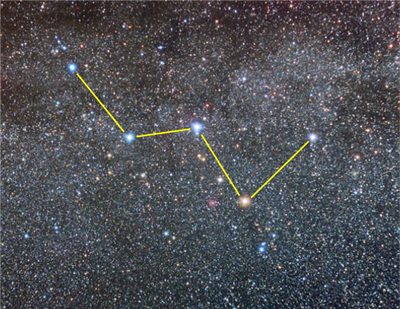
\includegraphics[width=3in]{images/Cassiopeia.png}
\end{center}
\end{figure}
\vspace{1cm}

\begin{quotation}
"For [Kassiopeia], the wife of Cepheus, vied with the Nereids in beauty and boasted to be better than them all; hence the Nereids were angry, and Poseidon, sharing their wrath, sent a flood and a monster to invade the land..."\\

{\it --from Apollodorus, Bibliotheke II, iv, 3}
\end{quotation}
\end{center}



\tableofcontents{}

% Introduction for the Kassiopeia Guide

\chapter{Introduction}\label{sec:introduction}

\textsc{Kassiopeia} is the primary simulation package for the KATRIN Experiment.  It is written primarily in C++, and is comprised of modules for particle creation, particle trajectory calculation in electro-magnetic fields, particle detection and data acquisition. A variety of different particle generators (see Section~\ref{KPAGEmain}) and different tracking methods are available. Physical processes like synchrotron radiation, scattering can be taken into account (see Section~\ref{sec:KTrack}). The particle detection module includes backscattering of electrons on the detector surface as well as a comprehensive number of physical phenomena of low energetic electrons in silicon (see Section~\ref{KESSMain}). DAQ is not available in this version of \textsc{Kassiopeia}. The user interface is via configuration files and output is written into \cernroot{} files.

The Monte Carlo simulations performed with \textsc{Kassiopeia} should be applicable for three purposes: 
\begin{enumerate}
\item Answering design questions for KATRIN. For instance, the influence of a gap in the wire electrode system on the background could be studied with \textsc{Kassiopeia}.
\item \textsc{Kassiopeia} will be used for near-time simulations, in the commissioning and data-taking phases of KATRIN. This will give the experimenters the ability to quickly check or preview of the measurements.
\item Finally, with the help of Monte Carlo simulations with \textsc{Kassiopeia}, the systematic uncertainties for a neutrino-mass measurement can be estimated.
\end{enumerate}




% How to use Kassiopeia
\chapter{How-To Guide}\label{ch:howto}

In this section the basic information about how to get, configure and run \textsc{Kassiopeia} are explained.
Usful information about \textsc{Kassiopeia} can also be found on the KATRIN wiki: \url{https://wiki.fzk.de/katrin/index.php/Kassiopeia}. Once \textsc{Kassiopeia} is installed, you also have access to the Doxygen-based reference manual.

Please note that throughout this guide the top-level directory of the \textsc{Kassiopeia} distribution will be referred to as \texttt{<maindir>}.


\section{Latest Version: 1.20.00}


\section{System Requirements}
\textsc{Kassiopeia} has been tested on Linux and MacOS systems.  Windows is currently not supported.  Several versions of gcc 4.x have been tested; gcc 3.2 does not work.

Be sure that you have the following packages and minimum versions installed on your computer:
\begin{itemize}
	\item \cernroot{} 5.24 or higher
	\item GSL 1.0 or higher
	\item boost 1.34 or higher
\end{itemize}


\section{Getting \textsc{Kassiopeia}}
You have two options for downloading any distribution of \textsc{Kassiopeia}:
\begin{description}
\item[Distribution Tarball]

For every \textsc{Kassiopeia} release there will be a tarball of the full distribution.  This can currently be downloaded from the M\"unster SVN repository (a better location will be found in the future).  The suggested method for doing this is via the web interface: \url{https://nuserv.uni-muenster.de/viewvc/Kassiopeia/tar}.  From there you can download the file \texttt{kassiopeia-X.YY.ZZ.tar.gz}, and place it in the directory in which you want to unpack it.
\begin{DoxyCode}
>  tar -xzvf kassiopeia-X.YY.ZZ
>  cd kassiopeia-X.YY.ZZ
\end{DoxyCode}
This is the simplest method for obtaining a copy of \textsc{Kassiopeia}.  It is also independent of the Autotools suite, so it is recommended for installing on older operating systems or systems which do not have the required versions of autoconf, automake, or libtool (see below).

\item[SVN Check-Out]

\textsc{Kassiopeia} source can be found on the KATRIN SVN repository at the University of M\"unster (\url{https://nuserv.uni-muenster.de/svn/katrin/}).  You must have an account to install \textsc{Kassiopeia} in this way, you must have the following versions of the Autotools applications:
\begin{itemize}
\item autoconf v2.65 or higher, earlier versions may work, but we make no promises
\item automake v.1.10, recommended 1.11 or higher. 
\item libtool v. 2.2, earlier versions may work, but again, no promises 
\end{itemize}

The distribution can be obtained from the SVN repository in the standard way:
\begin{DoxyCode}
>  svn co https://nuserv.uni-muenster.de/svn/katrin/Kassiopeia/tags/kassiopeia-X.YY.ZZ
>  cd kassiopeia-X.YY.ZZ
\end{DoxyCode}

\end{description}


\section{Installing \textsc{Kassiopeia}}

\subsection{Configuring the Installation}
These commands are run from \texttt{<maindir>}.

If you used the \textbf{SVN Check-Out} method (not using the tarball) to obtain \textsc{Kassiopeia}, then the \texttt{configure} script and Makefiles still need to be created via the Autotools suite.  The \texttt{autogen.sh} script will take care of this, as well as running the \texttt{configure} script.  From the command line, run:
\begin{DoxyCode}
>  ./autogen.sh
\end{DoxyCode}

For those who used the \textbf{Distribution Tarball} method to obtain \textsc{Kassiopeia}, the \texttt{configure} script already exists.  Simply run it from the command line:
\begin{DoxyCode}
>  ./configure
\end{DoxyCode}

The rest of these instructions apply to \textbf{both} methods of obtaining \textsc{Kassiopeia}, except as noted.

If you would like to see the available installation options, type
\begin{DoxyCode}
>  ./configure --help
\end{DoxyCode}
If necessary, run the configure script again with any desired customized options.

For example, to install \textsc{Kassiopeia} in another directory than the current one, use 
\begin{DoxyCode}
 > ./configure --prefix=/path/to/some/directory
\end{DoxyCode}

\subsection{Compiling and Installing}

From \texttt{<maindir>}, type the following two commands to, respectively, compile and install \textsc{Kassiopeia}:
\begin{DoxyCode}
>  make
>  make install
\end{DoxyCode}
If everything compiles and installs correctly, \textsc{Kassiopeia} is ready to use.


\section{Running \textsc{Kassiopeia}}
The primary \textsc{Kassiopeia} executable, which performs tracking simulations, is called \texttt{Kassiopeia}.  It is installed in \texttt{<maindir>/bin} in a standard installation.

Before you really configure your own simulation you can do a little test run with \textsc{Kassiopeia}. Run the following:
\begin{DoxyCode}
>  <maindir>/bin/Kassiopeia
\end{DoxyCode}
The default run is a single event, where an electron is emitted from an electron gun.  You will see a warning printed because you did not provide a UserConfiguration file.  This file is the primary user interface.  One way to avoid this warning is to supply the name of the UserConfiguration file you want to use:
\begin{DoxyCode}
>  <maindir>/bin/Kassiopeia <maindir>/etc/UserConfiguration.txt
\end{DoxyCode}
Either way you run \textsc{Kassiopeia}, three files will be created in your current directory: the output, named \texttt{KassiopeiaOutput.root} by default, and the log and error files.  
You can open \texttt{KassiopeiaOutput.root} with \cernroot. With the help of the TreeViewer of \cernroot{} you can have a look at the particle's trajectory.


\section{Configuring \textsc{Kassiopeia}}
\textsc{Kassiopeia} is controlled with a set of configuration files.  This is true for both the Kassiopeia executable as well as other applications.  This section describes how to configure the tracking simulation (the Kassiopeia executable), but much of the information is relevant to configuring other applications that use the \textsc{Kassiopeia} management structure, as well.

The primary user interface for \textsc{Kassiopeia} is via the UserConfiguration file and the command line.  The setup of the simulation is done in the KassiopeiaConfiguration file.  The tools that are used in the simulation are composed with the toolbox configuration files.

Examples of all of the configuration files are found in \texttt{<maindir>/etc}.  For your own simulations your should make local copies of any configuration files you need to modify in a local directory; with every update of \textsc{Kassiopeia} the default files in \texttt{<maindir>/etc} are overwritten and any changes to them will be lost.  The locations for the local copies of the configuration files can be specified as described in section~\ref{sec:howto-userconfig}.

The syntax of all configuration files is XML-like: First you define \textbf{what} you want to configure in a block known as a configuration ``element.''  The syntax uses single angle brackets: \texttt{$<$THING TO CONFIGURE$>$}. \texttt{$<$/THING TO CONFIGURE$>$} denotes the end of the element. Parameter settings are written with double angle-brackets: \texttt{$<<$PARAMETER=VALUE$>>$}.

Here is an example of the configuration file syntax:
\begin{DoxyCode}
#this is a comment

/*
and this is
a block comment
*/

<Element1>                      #The beginning of an element for the Kassiopeia class being configured
    <<Name=name1>>              #Every element with parameters must be named first
    <<Parameter1Name=Value1>>   #A basic parameter being set to Value1
    <<Parameter2Name=Value2>>   #Another parameter being set to Value2
</Element1>                     #The end of the element for the class

<Element2>
    <<Name=name2>>
    <SubElement>                #A nested element
        <<Name=subname>>
        <<Parameter3Name=Value3>>
    </SubElement>
</Element2>
\end{DoxyCode}
As can be seen in the example, there are two ways to denote a comment, either in a line or a block.  Every element (with only a few exceptions) must have a \texttt{Name} as the first parameter.  These names must be unique in the global Kassiopeia parameter space.  Elements can also be nested (and those sub-elements also must have \texttt{Name}s.  Please browse through the configuration files that come with \textsc{Kassiopeia} to see what this looks like in practice.

In addition to the above syntax, the user can communicate directly with the system that reads the configuration files (the Tokenizer).  This is done via keyword commands.  The syntax is:
\begin{DoxyCode}
@keyword(comma,separated,arguments)
\end{DoxyCode}

Available keywords:
\begin{description}
	\item[include] Configurations can be split up among multiple files, and the files can be included from one another.  This keyword takes only one argument, the file name. This allows for more flexibility and reusability in making configuration files.  So, for example, perhaps you want to split the GeometryConfiguration into multiple files, each of which describes one region of the system being simulated.  GeometryMaster.txt brings all of the files used together:
\begin{DoxyCode}
@include(GeometryRegion1.txt)
@include(GeometryRegion2.txt)
\end{DoxyCode}
This keyword can only be used outside of any configuration element blocks.
\end{description}
 


\subsection{UserConfiguration and KassiopeiaConfiguration}\label{sec:howto-userconfig}
\subsubsection{UserConfiguration}
The default filename for the UserConfiguration file is \texttt{UserConfiguration.txt}.  When you run \textsc{Kassiopeia}, the UserConfiguration file will be found with one of the following ways (in order of priority, from highest to lowest):
\begin{enumerate}
	\item You can specify the UserConfiguration file with the first argument on the command line.
	\item \textsc{Kassiopeia} will look for \texttt{<maindir>/etc/UserConfiguration.txt}.
	\item If no UserConfiguration file is specified or found, the application will exit.
\end{enumerate}

The UserConfiguration file includes the following settings: 
\begin{itemize}
	\item The verbosity level
	\item Direct settings
	\item Variable replacement
	\item Default configuration file and data file directories
	\item Local configuration files
\end{itemize}
This particular order of the settings is highly recommended, though not fundamentally required.

\subsubsection{Verbosity}
The verbosity level defines what is printed to screen and written into a log file. Seven verbosity levels are available:
\begin{itemize}
	\item Error: Only error messages are printed  
	\item Warning: in addition warning are printed  
	\item GlobalMessage: in addition global messages, like which configuration files are used, are printed
	\item RunMessage: in addition all messages occurring on run level are printed  
	\item EventMessage: in addition all messages occurring on event level are printed 
	\item TrackMessage: in addition all messages occurring on track level are printed 
	\item Debug: in addition debug messages are printed. In this case you have to enable the debug of the part you are interested in before compiling. \texttt{<maindir>/configure --help} shows you the options. If your program was already compiled you have to run \texttt{make clean} before recompiling.
\end{itemize}

\subsubsection{Direct Parameter Settings}
These settings allow you to change the values of parameters in the toolbox configuration files and the KassiopeiaConfiguration file without modifying the files themselves.  You only need to know the configuration element name and the name of the parameter that is being set.  This is particularly convenient if you want to change a parameter's value often.  The notation is:
\begin{DoxyCode}
<DirectSetting>
    <<ParameterLocation1=Value1>>
    <<ParameterLocation2=Value2>>
    ...
</DirectSetting>
\end{DoxyCode}
The location of a parameter is the combination of the configuration element name, and the parameter name: \texttt{ElementName:ParameterName}.

So, for instance, if you want to change the run number, and the name of the RunConfiguration element is RunConfig, then you would place the following in UserConfiguration:
\begin{DoxyCode}
<DirectSetting>
    <<RunConfig:RunId=12345>>
</DirectSetting>
\end{DoxyCode}
This value for the run number will then overwrite whatever is actually in the KassiopeiaConfiguration file (where the RunConfiguration element lives).

\subsubsection{Variable Replacement}
These settings allow you to change the values of parameters in the toolbox configuration files and the KassiopeiaConfiguration file (or even the portion of the UserConfiguration file after the variable is defined) while only modifying the UserConfiguration file.  You define a variable in the UserConfiguration file, and then use that variable instead of a parameter value in the other configuration file.  This is particularly convenient if you want to change a parameter's value often.

For instance, you might define a variable for the run number in the UserConfiguration file:
\begin{DoxyCode}
<ParameterReplacement>
    <<RunNumber=12345>>
    /* <<VARIABLE=VALUE>> <-- General syntax */
</ParameterReplacement>
\end{DoxyCode}
Then, in the KassiopeiaConfiguration file (under \texttt{$<$RunConfiguration$>$}) you would replace the run number value with \texttt{\$\{RunNumber\}}:
\begin{DoxyCode}
<<RunId=${RunNumber}>>
\end{DoxyCode}
When the KassiopeiaConfiguration file is loaded, the variable will be replaced by the value defined in the UserConfiguration file.

\subsubsection{Default Configuration File and Data File Directories}
The default directories for configuration files and data files can be set from the UserConfiguration file.  These settings are stored in the KSCoreManager.

For the configuration files, they are not required to be located in this directory.  Please see section~\ref{sec:howto-specifyingconfigfiles} for details on how each configuration file is found by \textsc{Kassiopeia}.

You can define the local directories in this way:
\begin{DoxyCode}
<PreliminaryConfiguration>
    <<OptionHome=[path]/MyConfigFiles>>
    <<DataHome=[otherpath]/DataFiles>>
</PreliminaryConfiguration>
\end{DoxyCode}

Configuration files and data files in these directories (respectively) must have the default file names.

\subsubsection{Local Configuration Files}
You can also specify individual configuration files (except for UserConfiguration, obviously) in the UserConfiguration file. This setting has highest priority when \textsc{Kassiopeia} locates configuration files.  Note that the filenames, when individually specified, do not have to be the same as the default file names (e.g. you could rename your copy of \texttt{GeometryConfiguration.txt} to be \texttt{GeometryConfiguration\_revision8.txt}).

You specify a configuration file in this way:
\begin{DoxyCode}
<ConfigFile>
    <<Generator=[path]/MyConfigFiles/MySpecialGeneratorConfiguration.txt>>
    /* <<KEY=FILENAME>>  <-- General syntax */
</ConfigFile>
\end{DoxyCode}
The available keys are: \texttt{Global, Kassiopeia, DAQ, Field, Generator, Geometry, SSC,} and \texttt{StepStrategy}.


\subsubsection{Command Line}
Anything that can be set in the UserConfiguration.txt file can be set from the command line.  The command-line settings will take precedence over the UserConfiguration file if something is specified in both places.
The command-line syntax is:
\begin{DoxyCode}
>  Kassiopeia  [UserConfiguration file]  [-d [Direct parameter settings]] 
[-r [Parameter variable replacements]]  [-c [Local Configuration files]] 
[-t [Other tokens]]
\end{DoxyCode}

\begin{description}
	\item[\texttt{[UserConfiguration file]}] Setting the UserConfiguration file is optional, but if it's specified it must be the first argument in the command line.  Simply give the file location (either relative to the run location or the absolute path) and name.
	\item[\texttt{[-d [Direct parameter settings]]}] The -d flag can be used to easily specify direct parameter settings without using the full syntax (see -t below).  The syntax for this is:
	\begin{DoxyCode}
	-d LOCATION1=VALUE1 LOCATION2=VALUE2
	\end{DoxyCode}
	where a location is the combination of the configuration element name and the parameter name: \texttt{ElementName:ParameterName}.
	\item[\texttt{[-r [Parameter replacements]]}] The -r flag can be used to easily specify parameter replacement variables without using the full syntax (see -t below).  The syntax for this is:
	\begin{DoxyCode}
	-r VARIABLE1=VALUE1 VARIABLE2=VALUE2
	\end{DoxyCode}
	\item[\texttt{[-c [Local Configuration files]]}] The -c flag can be used to easily specify local configuration files without using the full syntax (see -t below).  The syntax for this is:
	\begin{DoxyCode}
	-c KEY1=FILENAME1 KEY2=FILENAME2
	\end{DoxyCode}
	The available keys can be found in the UserConfiguration.txt file that is included with \textsc{Kassiopeia}.
	\item[\texttt{[-t [Other tokens]]}] Any tokens usually in the UserConfiguration file can be given under the -t flag in the command line. As an example to demonstrate the syntax, you would set the verbosity and configuration file directory as:
	\begin{DoxyCode}
	>  Kassiopeia -t --PreliminaryConfiguration VerbosityLevel=Run 
	OptionHome=[some directory path] ++
	\end{DoxyCode}
	Note that the `\texttt{++}' at the end indicates the end of the PreliminaryConfiguration block, and is necessary.  This syntax does support the nesting of tokens, but right now that's not applicable to the UserConfiguration settings.  Both the parameter replacement variables and the local configuration files could be specified using this notation, but the \texttt{-r} and \texttt{-c} options are available so you can use their simpler syntax.
\end{description}

\subsubsection{KassiopeiaConfiguration}
This configuration file is used to specify exactly what you want to simulate.  It is divided into several parts: global (currently in a separate file), run, event and track settings.  These set up \textsc{Kassiopeia} to use the tools that are described below.
\begin{itemize}
	\item Global: Definition of random seed, output file, output file format, output level (currently in the GlobalConfiguration file)
	\item Run: Definition of the number of particles you want to simulate and the time of run
	\item Event: Definition of generators used for this run
	\item Track: Definition of regions and their corresponding step strategies
\end{itemize}
The corresponding configuration file, by default called \texttt{KassiopeiaConfiguration.txt}, is quite short, since for both event and track configuration you simply refer to the tools you configured earlier by name.

Here is an example of how the event configuration is set:
\begin{DoxyCode}
<EventConfiguration>
    <<use=MyEgun>> 
</EventConfiguration>
\end{DoxyCode}
In this configuration the generator chosen for the run is called ``MyEgun.''  That generator, assuming it is provided in the GeneratorConfiguration file, will be used for all events.  Multiple generators can be specified for more complicated run setups.  Each is assigned a ``weight''; the generator that initiates a particular event is chosen randomly based on those weights.

The \texttt{TrackConfiguration} section is used to define the regions and their corresponding computation strategies.  \textsc{Kassiopeia} offers the possibility to change computation method depending on the position of the particle. For instance, close to electrodes a smaller step size can be chosen. As another example, \textsc{Kassiopeia} can switch from the simulation of particles in vacuum to a simulation of particles in silicon once the particle hits the detector.


\subsection{Toolbox Configurations}
The other configuration files are used to configure the tools that are needed throughout the simulation. For this purpose four configuration files can be adjusted. The configuration files, with their default file names and the topics they address, are:
\begin{description}
	\item[GeneratorConfiguration] (\texttt{GeneratorConfiguration.txt}): How are the particles generated?
	\item[SSCConfiguration] (\texttt{SSCConfiguration.txt}): How is the tritium source configured?
	\item[StepStrategyConfiguration] (\texttt{StepStrategyConfiguration.txt}): How is the trajectory computed and which exit conditions should be used?
	\item[FieldConfiguration] (\texttt{FieldConfiguration.txt}): Which magnetic and electric fields are present and with which method should they be computed?
	\item[GeometryConfiguration] (\texttt{GeometryConfiguration.txt}): Which geometrical shapes are needed for particle generation, navigation and exit conditions?
	\item[DAQConfiguration] (\texttt{DAQConfiguration.txt}): Not currently in use.
\end{description}

Each tool is given a ``Name'' so that it can be referred to in the KassiopeiaConfiguration file, and so that different instances of the same type of tool can be identified within the simulation.

Here is an example of how you would configure the angular-defined e-gun generator:
\begin{DoxyCode}
<PAGEGeneratorADEgun>
    <<Name=MyEgun>> 
    <<Weight=1>>
    <<StartPositionX=0.>>
    <<StartPositionY=0.>>
    <<StartPositionZ=-2.24.>>
    <<MeanEnergy=18000.>>
    <<SigmaEnergy=100.>>
    <<MeanTheta=0.0>>
    <<SigmaTheta=0.01>>
    <<MeanPhi=0.0>>
    <<SigmaPhi=0.01>>
</PAGEGeneratorADEgun>
\end{DoxyCode}

\subsubsection{Specifying Configuration Files}\label{sec:howto-specifyingconfigfiles}
\textsc{Kassiopeia} searches for the correct configuration files in a particular way.  The hierarchy used is as follows, for any particular configuration file (besides UserConfiguration):
\begin{enumerate}
	\item It checks if you defined a local configuration file in \texttt{UserConfiguration.txt}. This setting has the highest priority.
 	\item If you did not specify the configuration file, \textsc{Kassiopeia} will check in the current directory (from which the simulation is being run) for a file with the default name.
	\item If it does not find the default filename in the current directory it will look in the directory specified as the configuration file directory.  That setting can be made in one of three ways (also in order of priority, from high to low):
	\begin{enumerate}
		\item You can specify the directory from the \texttt{PreliminaryConfiguration} section of the UserConfiguration file (see the default file for an example).
		\item If the directory is not specified in the UserConfiguration file, then it can come from the \texttt{KSCONFIG} environment variable.  The script \texttt{<maindir>/Applications/Scripts/setenv.(c)sh} can be sourced from your shell login script to make this convenient if you usually use the same \textsc{Kassiopeia} installation.  The environment variable \texttt{KSDATA} can also be used to define the data file directory.
		\item If \texttt{KSCONFIG} is not set and the directory is not specified from the \texttt{UserConfiguration} file, then the default value in KSCoreManager will be used.  This will be set to the value of the variable \texttt{sysconfdir} while \textsc{Kassiopeia} is being built (Use \texttt{<maindir>/configure --help} from the command line to see how to set this).
	\end{enumerate}
	\item If the configuration file can not be found there the program will quit with a fatal error. 
\end{enumerate}


\subsubsection{Available Tools}
The following lists are the complete set of tools currently available in \textsc{Kassiopeia}, along with the default file names for the configuration files in which they are located.
\begin{description}
	\item[Generator Toolbox] (\texttt{GeneratorConfiguration.txt}):
	\begin{itemize}
		\item Particles start at fixed position, energy and angles (\texttt{PAGEGeneratorFix})
		\item Angular defined egun (\texttt{PAGEGeneratorADEgun})
		\item Approximation of WGTS (\texttt{PAGEGeneratorFastWGTS})
		\item Real WGTS (\texttt{PAGEGeneratorWGTS})
		\item Radon 219 and 220 decay (\texttt{PAGEGeneratorRadon})
		\item Tritium decay (\texttt{PAGEGeneratorTritim})
		\item Krypton decay (\texttt{PAGEGeneratorKrypton})
		\item Particle starting from a user defined surface (\texttt{PAGEGeneratorSurface})
		\item Particle starting in a user give volume (\texttt{PAGEGeneratorVolume})
	\end{itemize}
	\item[Step Strategy Toolbox] (\texttt{StepStrategyConfiguration.txt}):
	\begin{itemize}
		\item Three different stepping modes are available:
		\begin{itemize}
			\item Exact stepping method (\texttt{KTrackExactStepComputer})
			\item Adiabatic approximation method (\texttt{KTrackAdiabaticStepComputer})
			\item Stepping method valid in silicon (\texttt{KESSStepComputer})
		\end{itemize}
		\item One can think of the KTrack stepping modes as empty boxes that can be filled with different processes:
		\begin{itemize}
			\item Propagation (Runge Kutta 8, Predictor Corrector or Embedded Runge Kutta)
			\item Gyration (only possible for adiabatic stepping method)
			\item Drift (only possible for adiabatic stepping method)
			\item Synchrotron
			\item Scattering
		\end{itemize}
		\item The KTrack stepping modes can have different step-size-controlling methods. Multiple selection is possible.
		\begin{itemize}
			\item Fixed time step
			\item Maximal step length
			\item Fraction of cyclotron period
			\item Limit on energy conservation violation
			\item Maximal scattering probability
			\item Maximal synchrotron energy lost
			\item Limit on numerical error (only available for embedded Runge Kutta methods)
		\end{itemize}
		\item A variety of exit conditions are available:
		\begin{itemize}
			\item Maximal number of steps
			\item Maximal path length
			\item Maximal z position
			\item Detector hit
			\item Geometry hit
			\item After a certain number of turns
			\item After a certain number of full magnetron turns
			\item ... more problem-specific exit conditions are available
		\end{itemize}
	\end{itemize}
	\item[Field Calculation Toolbox] (\texttt{FieldConfiguration.txt}):
	\begin{itemize}
		\item Electric field calculation methods:
		\begin{itemize}
			\item ELCD2 (Legendre polynomial expansion and elliptic integral method (automatic switch), valid for axially symmetric geometries, wire electrode is approximated as full cones) (\texttt{KAFCAElfield2Ferenc} or \texttt{KAFCAELCD2})
			\item ELCD32 (Legendre polynomial expansion and elliptic integral method (no automatic switch), valid for axially symmetric geometries) (\texttt{KAFCAElfield32Ferenc})
			\item ELCD33 (valid for non axially symmetric geometries, not fully tested) (\texttt{KAFCAELCD33})
			\item ELCD34 (not in this version)
			\item KEMField
			\item Constant (\texttt{ElfieldConstant})
			\item Hermite interpolation (\texttt{ElfieldInterpolate})
		\end{itemize}
	\item Magnetic field calculation methods:
		\begin{itemize}
			\item Magfield3 (Legendre polynomial expansion and elliptic integral method (automatic switch), valid for tilted cold) (\texttt{KAFCAMagfield3Ferenc})
			\item Constant (\texttt{KAFCAMagfieldConstant})
			\item Dipole (\texttt{KNAXSMagneticDiopoles})
			\item Bio Savart (\texttt{KNAXSBiotSavart})
			\item Hermite interpolation (\texttt{KNAXSMagfieldInterpolate})
		\end{itemize}    
	\end{itemize}
	\item[Geometries] (\texttt{GeometryConfiguration.txt}):\\
	In this first version of \textsc{Kassiopeia}, geometries can only be built from cones. Therefore you can define two types of objects:
	\begin{itemize}
		\item Cones
		\item Polycones
	\end{itemize}
\end{description}



\section{Looking at the Results}
Two output formats are available. The \textit{three tree} output and a \textit{TClonesArray} output. You choose the format in the \texttt{GlobalConfiguration.txt}. Also there, you can choose the output level: (event, track, step). In the output you correspondingly find information about events, tracks and steps. In the \textit{three tree} output these are just three trees, whereas in the TClonesArray format it is more complicated. In this version of \textsc{Kassiopeia} you configure the output via the output level and the modules, you are using in your simulation, themselves. For instance the Scattering module has a parameter ``output'' that can be set to 1 or 0 within the configuration of the Scattering module.

Furthermore a \texttt{TrackPlotter.cxx} will be available in \texttt{<maindir>/Applications/Other/src}, that plots the trajectory of the particles in a user defined geometry.

Additionally, a macro called FileReader is provided, which reads in the output file and allows the user to quickly insert his own analysis code there. In the future, this functionality will become part of KALI and will be expanded to full dynamically linked system for user defined analysis functions. 
It can be used as follows: First of all, start root. Then in root do: 
\begin{DoxyCode}
      root [0] .L /path/to/kassiopeia/bin/FileReader.C
      root [0] FileReader("/path/to/filename.root", "/path/to/kassiopeia/lib);
\end{DoxyCode}

The default behavior is just to print some not very interesting  information on the screen, but you can adapt it to fit your purposes.


% Simulation architecture documentation for the Kassiopeia Guide
\chapter{The \textsc{Kassiopeia} Architecture}\label{ch:architecture}

\section{Global Picture}
\label{arch:globalpicture}

The core of \textsc{Kassiopeia} is made up of pieces of code that fall into three principal categories:  Managers, Modules, and Data Containers.  This architecture is used by the main application (Kassiopeia, for tracking simulations), and other applications within \textsc{Kassiopeia}.  Most of this discussion will focus on the simulation but will be applicable to other applications as well.

The Data Containers are basic objects that simply represent the state of the simulation in computer memory as it is executing, and it is the responsibility of the Modules to initialize and update the contents of these Data Containers as simulation time progresses.  The Managers in turn organize and control which Modules are active at which time.

Managers come in two varieties: Toolboxes and `Execution' Managers.  Toolboxes simply collect and organize available Modules, and Execution Managers connect the Modules in the Toolboxes together and use them to progress the simulation.   

The Data Containers are organized into four physically intuitive levels of detail:  Runs, Events, Tracks, and Steps.  Since it is the job of the Modules and Managers to figure out how to update these Data Containers as time progresses, this organizational principle naturally extends to the rest of \textsc{Kassiopeia}, too.  It is therefore worthwhile to describe in detail how interesting simulation information falls into these four categories.

\section{Simulation Organization}
\label{arch:simorganization}

\subsection{Runs}
\label{arch:runs}

The Run organization level is the highest level, and represents everything that happens during one execution of \textsc{Kassiopeia}.  A Run is not much more than a collection of Events, and global information that only pertains to Runs is limited to the number of events that occur in a run and how much physical time elapsed during the period of the Run.  It is important to note that no physical parameters of the simulation may change during a Run.  This includes but is not limited to high-voltage settings, magnet currents, and the like.  Therefore, the present \textsc{Kassiopeia} definition of Run is in line with the Katrin experimental definition of a Subrun.  Support for real experimental Runs and the consequently necessary name change will be added in a future version.

\subsection{Events}
\label{arch:events}

The Event organization level matches what one would intuitively think: a physical process occurs to generate one or more primary particles, whose states are represented by Tracks, and all of the things that happen as a consequence of these Tracks and their secondary Tracks are grouped together into an Event.  In \textsc{Kassiopeia} there is one type of Module devoted to the creation of the inital state of these primary Tracks, called a Generator.  The name of our package of Generators is KPAGE (KATRIN PArticle GEnerator), and technical details about how these Modules work can be found in the KPAGE section of this document.

\subsection{Tracks}
\label{arch:tracks}

The Track organization level, as alluded to before, represents information about the physical particles that \textsc{Kassiopeia} aims to simulate.  To be precise, in \textsc{Kassiopeia} a Particle is an instantaneous \emph{physical} state of a Track, defined by a position vector, a momentum vector, rest mass, charge, spin, lifetime, and and particle type ID number.  These ID numbers match the PDG standard where defined for particular species.  Tracks in \textsc{Kassiopeia} contain two Particle states each: one for the initial state, and one for the current state which gets updated as the simulation runs.  Tracks also contain additional, non-physical simulation information, including an ID number that is unique and causally sequential within an event, a stamp indicating the physical process that created the Track, and the ID number of a parent Track.  In the case that a particle is primary and directly created by a Generator Module (thus having no parent Track), this ID has the value -1.  Finally, Tracks also have available their path length, their elapsed time, the number of steps used in their calculation, and a stamp indicating the reason \textsc{Kassiopeia} stopped the Track.  In \textsc{Kassiopeia}, the modules associated with the Track level are geometrical objects, called Regions, described in section \ref{arch:geometry}.  These are special Modules that represent user instructions for what physical processes \textsc{Kassiopeia} should simulate.

\subsection{Steps}
\label{arch:steps}

The Step organization level is the finest level of detail considered in \textsc{Kassiopeia}.  A Step is an incremental, discrete change to a Track.  In most applications it has two conceptual parts, the first being the numerical solution to an equation of motion, and the second being the simulation of discrete physical processes that may have occurred during flight along the step.  Steps keep track of their initial physical state, again represented as a Particle, and their final physical state, which, if the Step is acceptable, becomes the most current physical state of the Track to which the Step belongs.  As with the case for Events and their Generators above, \textsc{Kassiopeia} has several types of Modules whose responsibilities fall within the scope of calculating Steps.  The first of these is the Process type of Module, which is responsible for actually calculating the final Particle states within a Step.  Working closely with these Processes is the Step Size type of Module, which cooperate to determine the largest possible time increment over which a set of Processes may accurately act.  The last type of Module working at Step scope is the Exit Condition, which can indicate that a Step is the final one \textsc{Kassiopeia} will calculate for a given Track.  The suite of Processes, Step Sizes and Exit Conditions currently used in Kassopeia are documented in the KTrack section, with the exception of KESS which is a specifically designed process used for tracking in silicon.

\section{Geometry}
\label{arch:geometry}

Geometrical information is of course necessary in any particle tracking simulation.  In \textsc{Kassiopeia}, geometrical information is utilized in two distinct ways.  First, in the more local of the two ways, geometry is used as configuration information for modules.  For instance, field calculation Modules need to know where electrodes and magnets are, or a Generator Module might need to know the dimensions of a container filled with Radon.  In the more global usage, however, \textsc{Kassiopeia} associates configurations of Step level Modules with geometrical objects, essentially mapping out a geometry based plan of how to compute tracks and steps.  As mentioned above, such a binding between a geometrical object and a computation strategy is a special Track-level Module called a Region.

The basic Geometry objects themselves are oriented in a global \textsc{Kassiopeia} coordinate system, and are able to do all purely geometrical calculations required for simulation.  This includes determining whether a point is inside of the object or not, and a computation of the shortest distance to the object from a point.  The shapes available in \textsc{Kassiopeia} are currently limited to truncated cones and cylinders, as cylinders are a special limiting case of truncated cones.  This will be expanded in the next version, as will the calculations available in the Geometry objects in general.

\subsection{Regions}
\label{arch:regions}

A set of Regions in \textsc{Kassiopeia} is always a properly nested set of volumes, meaning that any Region may have sub-Regions which are completely contained within the parent Region without overlapping its boundaries.  Similarly, sub-Regions that are contained inside a parent Region may not overlap either.  This restriction on the geometries defining Regions allows the Regions to be organized in a tree-like way, with a single, special Region at the base of the tree.  This special Region is called the Root Region, and it physically contains all other Regions used and has no parent itself.  The tree structure of the Regions also is the way Regions are represented in the code of \textsc{Kassiopeia}:  each Region can be queried for its parent Region, and also for its set of child Regions.  A picture of a properly nested set of cylindrical Regions and the in-memory representation of this structure appears in figure \ref{archfig:geometry}.

\begin{figure}[!htb]
\centering
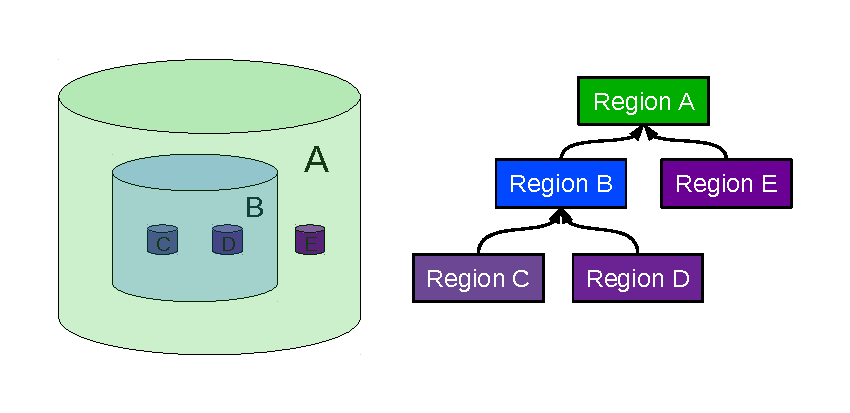
\includegraphics[width=0.7\textwidth]{images/ArchitectureFigures/ArchGeometry.pdf}
\caption{The geometrical and in-memory structure of Regions in \textsc{Kassiopeia}}
\label{archfig:geometry}
\end{figure}

The association between Regions and Step-level Module configurations is realized through a programming idea called the Command pattern.  In this pattern, a Command to switch configuration is itself saved, along with the Module being added or the name of the module being removed.  Such a saved Command is in a ready-to-execute state, and may be finally executed at any time, by any part of the code without that code needing to know the details of what the Command does.  This is done for speed reasons, since it saves having to retrieve a stepping Module from the Step Strategy Toolbox every time a configuration change is desired.  This is lookup is rather done one time during \textsc{Kassiopeia}'s execution during the initialization stage.  For each region, these Commands are separated into entry and exit commands, and each type is saved in an ordered list that may be accessed during computation.

\subsection{Navigation}

As a Track is being computed, \textsc{Kassiopeia} needs to know which Region the Track's current Particle state falls inside in order to load the proper Step computation Modules.  This is accomplished using a piece of code called the Navigator, which acts like an iterator for the tree structure of the regions.  As an iterator, it `sits' on the current Region occupied by the Track's Particle, and can travel up and down the branches of the tree structure as the Particle changes Regions as Tracks are updated.  As the Navigator traverses the tree, it builds up an ordered list of Commands to execute when it has completed its journey.

The basic algorithm for Navigation is recursive, and works as follows:

\begin{itemize}
\item The Navigator is given a Track's current Particle's position.
\item The Navigator determines whether this position is inside its current Region.
\item If it is still inside, the Navigator checks to see if the position is also inside one of the current Region's sub-Regions
    \begin{itemize}
        \item If so, the current Region is set to this sub-Region, the entry commands for the sub-Region are added to the list, and the function recurses.
        \item If not, or if there are no further sub-Regions, and the current Region is correct.
    \end{itemize}
\item If it is not still inside, the current Region is set to the parent Region, the exit commands for the old current Region are added to the list, and the function recurses.
\item If the position is outside of the root Region, an error is generated.
\end{itemize}

When the Navigator has finally oriented itself, it will have built up a list of configuration Commands to execute, gathered from nodes in the Region tree.  These Commands are directly executed by the Navigator as soon as the correct Region is found.

\section{CoreManager}
The entire management structure is overseen by the CoreManager (singleton).  The class KSCoreManager is a base class for application-specific derived classes.  For instance, KSCoreManagerSimulation is the CoreManager for the Kassiopeia application (tracking simulations).  Since this is a singleton class, only one CoreManager can exist at any given time.  Creation of the CoreManager is taken care of through the KSManagerFactoryTable.
 
KSCoreManager takes care of setting up the management hierarchy, and reading in the main configuration files.  It initiates the Setup and Prepare processes for all Managers and Toolboxes.  The specific derived CoreManager being used is responsible for specifying what the management structure will be (by choosing its downstream Managers), and performing the executing the actions taken by the application.  Again using KSCoreManagerSimulation as an example, the downstream Managers include KSRunManager, KSGeometryToolbox, KSFieldToolbox, SSCToolbox, KSGeneratorToolbox, KSStepStrategyToolbox, and KSDAQProcessorToolbox.  The Execute method creates and closes the output file, and runs the simulation.
 
The KSExceptionManager and the hierarchical structure of KSExceptionHandlers are responsible for writing log and error messages. They also cleanly handle situations where the simulation needs to shut down due to any sort of error.
 
The DataManager (singleton) is responsible for writing the output data.
 
The Management base class, KSManagerBase, provides the basic functionality common to all managers. These functions include those necessary to build (Setup()), navigate  (Get[Up/Down]streamManager()) and shutdown (ShutDown()) the tree-like management structure.  Furthermore, three other important functions are common to all managers:
\begin{itemize}
 \item Prepare()
 \item ProcessCommand()
 \item Execute()
\end{itemize}
 
Prepare() reads in the module configuration from the default or user-provided configuration file (if applicable), and generally gets the Manager or Toolbox ready for use in the simulation.
 
ProcessCommand() allows requests for configuration changes between managers to happen dynamically during the simulation (e.g. to change the field calculation method when entering another region of the experimental setup).  ProcessCommand() can deal with different types of inputs, given in form of KSBasicCommands, and is used for initialization and for configuration changes during a simulation.
 
Execute() causes the manager to perform its responsibilities on the data that is given as an argument.  Since each manager deals with different types of data, Execute() takes an arbitrary argument in form of a boost::any, and returns another arbitrary argument (again in the form of a boost::any*).  In contrast to KSManagerBase::ProcessCommand, KSManagerBase::Execute should typically only deal with one type of input, although that is not a strict requirement (for the experts: boost::anys provide intrinsic type information, which is its main advantage over void pointers as a solution for this kind of problem).
 
\section{Toolboxes}

Toolboxes are a type of Manager that stores configured Modules of \textsc{Kassiopeia}.  Since they are in the management chain, they are accessible from the CoreManager.  Each type of Toolbox has a configuration file associated with it, in which a user describes in detail a set of related Modules, each of which has a name.  When this configuration file is read, the Initializer/Builder system of \textsc{Kassiopeia} actually instantiates and configures the Modules described, and then registers them inside the Toolbox the system is set to work with. Other pieces of \textsc{Kassiopeia} can then query the Toolbox to retrieve these prepared modules.  Upon exit of \textsc{Kassiopeia}, Toolboxes are finally responsible for deleting all the modules they hold.

There are five types of Toolboxes associated with \textsc{Kassiopeia}:  Geometry, Field, SSC, Generator, and StepStrategy.  

\begin{itemize}

\item The Geometry Toolbox holds all the Geometry information used in calculations in \textsc{Kassiopeia}, as well as the Region modules that map out \textsc{Kassiopeia}'s computation strategy.  The Regions are stored simply by saving the root Region, with the sub-Regions stored directly in their natural tree structure.

\item The Field toolbox holds all the Modules involved in calculating electric and magnetic fields.  These Modules are typically used by other components in carrying out their responsibilities.  For instance, Modules involved in stepping need field information in order to evaluate the equations of motion, and some generators need to know the fields at initial points in order to calculate the momentum of particles.  

\item The SSC toolbox contains components of the SSC package of \textsc{Kassiopeia}, which is used in detailed simulations of the WGTS at Katrin.  SSC can perform detailed calculations of column density, as well as tritium spectra, and is principally used at the Event level of the architecture, but may also be used at the Step level for specific scattering calculations.  For more details, please see the SSC section.

\item The Generator toolbox naturally contains the Modules of \textsc{Kassiopeia} relevant for initializing Events and the Tracks they primarily contain.  There are a wide range of Generators available in \textsc{Kassiopeia}, with sources ranging from electron guns to radioactive volumes of gas. for more details on these and how they are configured, please see the KPAGE section of this document.  

\item The Step Strategy toolbox contains the three module types involved in calculating steps:  Step Sizes, Exit Conditions, and Processes.  These are exclusively used at the Step level to propagate particles.

\end{itemize}

For example, if there is a cone defined in Geometry Configuration file, a corresponding builder will create a cone object and configure it with the user defined values (e.g. radius). Then this object will be stored in the Geometry Toolbox together with other geometry objects. Technically, an add-function is used to store all these geometry objects in a geometry map and can later be accesed easily with a get-function.

In this way, all objects defined in the configuration files are created and placed in the corresponding toolbox.


\section{Rootclasses}

The Rootclasses are very similar to the Toolboxes. But whereas the Toolboxes contain all objects that have been defined in the configuration files, the Rootclasses only contain objects that are actually needed in the region the particle is currently in. So the content of the Rootclasses will be changed while the program is running, whereas the content of the Toolboxes is fixed in the initialization phase of the program. The regions, and the modules that should be used while the particle is inside these regions, can be defined in the \textsc{Kassiopeia} configuration file.

For example, all exit conditions that have been defined in the configuration files will be stored in the Step Strategy Toolbox. If a particle now enters a region, where the user only wants to use one of these exit conditions and has defined this in the \textsc{Kassiopeia} configuration file, the ExitCondition Rootclass will only content this object. Therefore, the function to check the exit conditions will automatically only check for this one.

But how will the content of the Rootclasses be changed while the program is running? After each step there will be a check if a new region has been entered or the current one has been left. In this case, a list of entry/exit commands, that have been created by the navigator (see chapter \textit{navigation} will be executed to change the content of the Rootclasses.


\section{Run, Event, Track, Step Managers}

Each level of the organizational structure in \textsc{Kassiopeia} has an associated Manager, referred to in the introductory paragraph as `Execution' Managers.  These managers drive simulation computation at their associated level.  Typically, the manager of a higher level will be responsible for creating an instance of the class used and filled in by a Manager of a lower level.  This is necessary because of the encapsulated nature of the architecture:  A manager of one level is responsible for calculating the contents of that object in isolation of other objects of the same type.  Therefore sequential id numbers of, say, Tracks can only be known at the overstanding Event level.

A pattern for the operation of these Managers occurs throughout the hierarchy (with a modification at the Step level done for speed).  First, an overstanding Manager creates an object of the type beneath it in the hierarchy, assigning it any sequential ids as necessary.  It then hands the prepared object to the next Manager type, which completely calculates the object it was given.  This process repeats itself until the original overstanding manager has created and completed all the objects it needs to have finished the object it was orignally given by its overstanding manager.  At the end of an object's calculation, it is told to write itself down, if configured to, by the manager that created it.  Finally, it is deleted.

The optimizing exception noted above for the case of the Step Manager is due to the typically very large number of Steps per Track in \textsc{Kassiopeia}.  At this level, the Track Manager makes a single Step object per Track it is given, then re-uses this Step object throughout the calculation of the current Track.

\section{Initialization}

\section{Output}
\begin{DoxyAttention}{Attention}
The source of this documentation can be found in: /KSCore/Main/KSCoreManager.h. some links will not work in the UserGuide, because there targets only exist in the ReferenceGuide.
\end{DoxyAttention}
The standard format for all output data is the \hyperlink{namespace_r_o_o_t}{ROOT} TTree. The output TTrees are stored in a TFile.

The output falls into three categories: \char`\"{}configuration\char`\"{}, \char`\"{}truth\char`\"{} and \char`\"{}real.\char`\"{}

The \char`\"{}configuration\char`\"{} data contains all the user specifications. That is necessary, because some if the configuration options may be set with the command line. However it is currently not existent, so you better keep track of your simulations....

The truth data includes all of the simulation-\/side information. This includes all information about all particles that were simulated, regardless of whether were actually \char`\"{}detected.\char`\"{}

The real data replicates what would be seen in an actual data file. It uses the same TTree format, and only includes information about detected events. Since the DAQ simulation is currently not functional, there is no real data tree in the \hyperlink{class_kassiopeia}{Kassiopeia} output files.

Two types of truth data are recorded: \char`\"{}physics\char`\"{} events and \char`\"{}DAQ\char`\"{} events. These are recorded in separate trees. Again, however, since the DAQ simulation is currently not functional, only the TTree of physics events is recorded.

The truth-\/side physics data can be written out in one of two different standardized formats, both of which reflect the event/track/step hierarchy. The output format is specified in the GlobalConfiguration file. 
\begin{DoxyItemize}
\item {\bfseries TClonesArray}: the TFile consists of a TTree of KMCEvents, which also include track and step data by using TClonesArrays. This is the standard output format, and it's faster than the ThreeTrees format. 
\item {\bfseries ThreeTrees}: the TFile consists of three trees, one for event, one for track and one for step data. This is primarily useful for simulations with large numbers of steps (e.g. trapped-\/particle studies), and as a more convenient format if you want to use the TTreeViewer in \hyperlink{namespace_r_o_o_t}{ROOT}. Otherwise it is slower than the TClonesArray format. 
\end{DoxyItemize}

The classes used to save the various blocks of data are different than the main KSEVent/KSTrack/KSStep classes. The output classes are called KMCEvent, KMCTrack, and KMCStep. The data are stored in blocks classes are KMCEventData, KMCTrackData, and a few different things for the steps.

The internal structure of the KMCEvent is rather non-\/intuitive, since for performance reasons during the saving, the data blocks inside an event have to have fixed size. A step in \hyperlink{class_kassiopeia}{Kassiopeia} is a rather complicated thing -\/-\/ different data may need to be saved depending on the active stepper and its internal state. Therefore the design of the output file structure has been challenging.


\begin{DoxyImage}
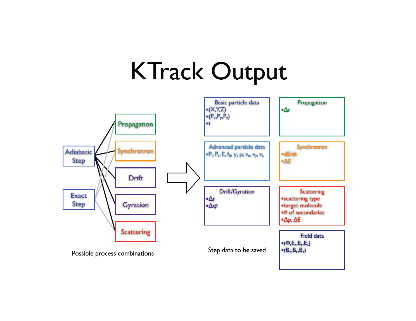
\includegraphics[width=\textwidth]{images/Output_fig1}
\caption{Tracking Step Output}
\end{DoxyImage}
 

The KMCStep class is special in the sense that its size in memory can change from one step to the next. e.g. you may chose to save scattering information only if a scattering interaction actually took place, or a process can be switched of and thus stop providing data altogether. For this reason, the step itself is split up in different fixed size blocks when it is written to disk and the KMCStep again has a non-\/trivial substructure. It consists of several Data blocks, which may or may not be present, and it's Save function knows how to deal with that. Simultaneously, it has a ReadNextStep block for accessing each step recursively. Note that the KMCStep class is strictly speaking not necessary, since it is not written to disk. it is only provided to encapsulate the complex step structure of a step within it.

The event structure as it is written to file is depicted in Fig.2: An event consists of an array of fixed sized blocks for the Track data, and presently eight fixed sized blocks which may of may not be written during each step. In order to retrieve a step from the track, the Trackdata block also contains a two-\/layered key system allowing the retrieval of step information. This key scheme is explained in the following figures:


\begin{DoxyImage}
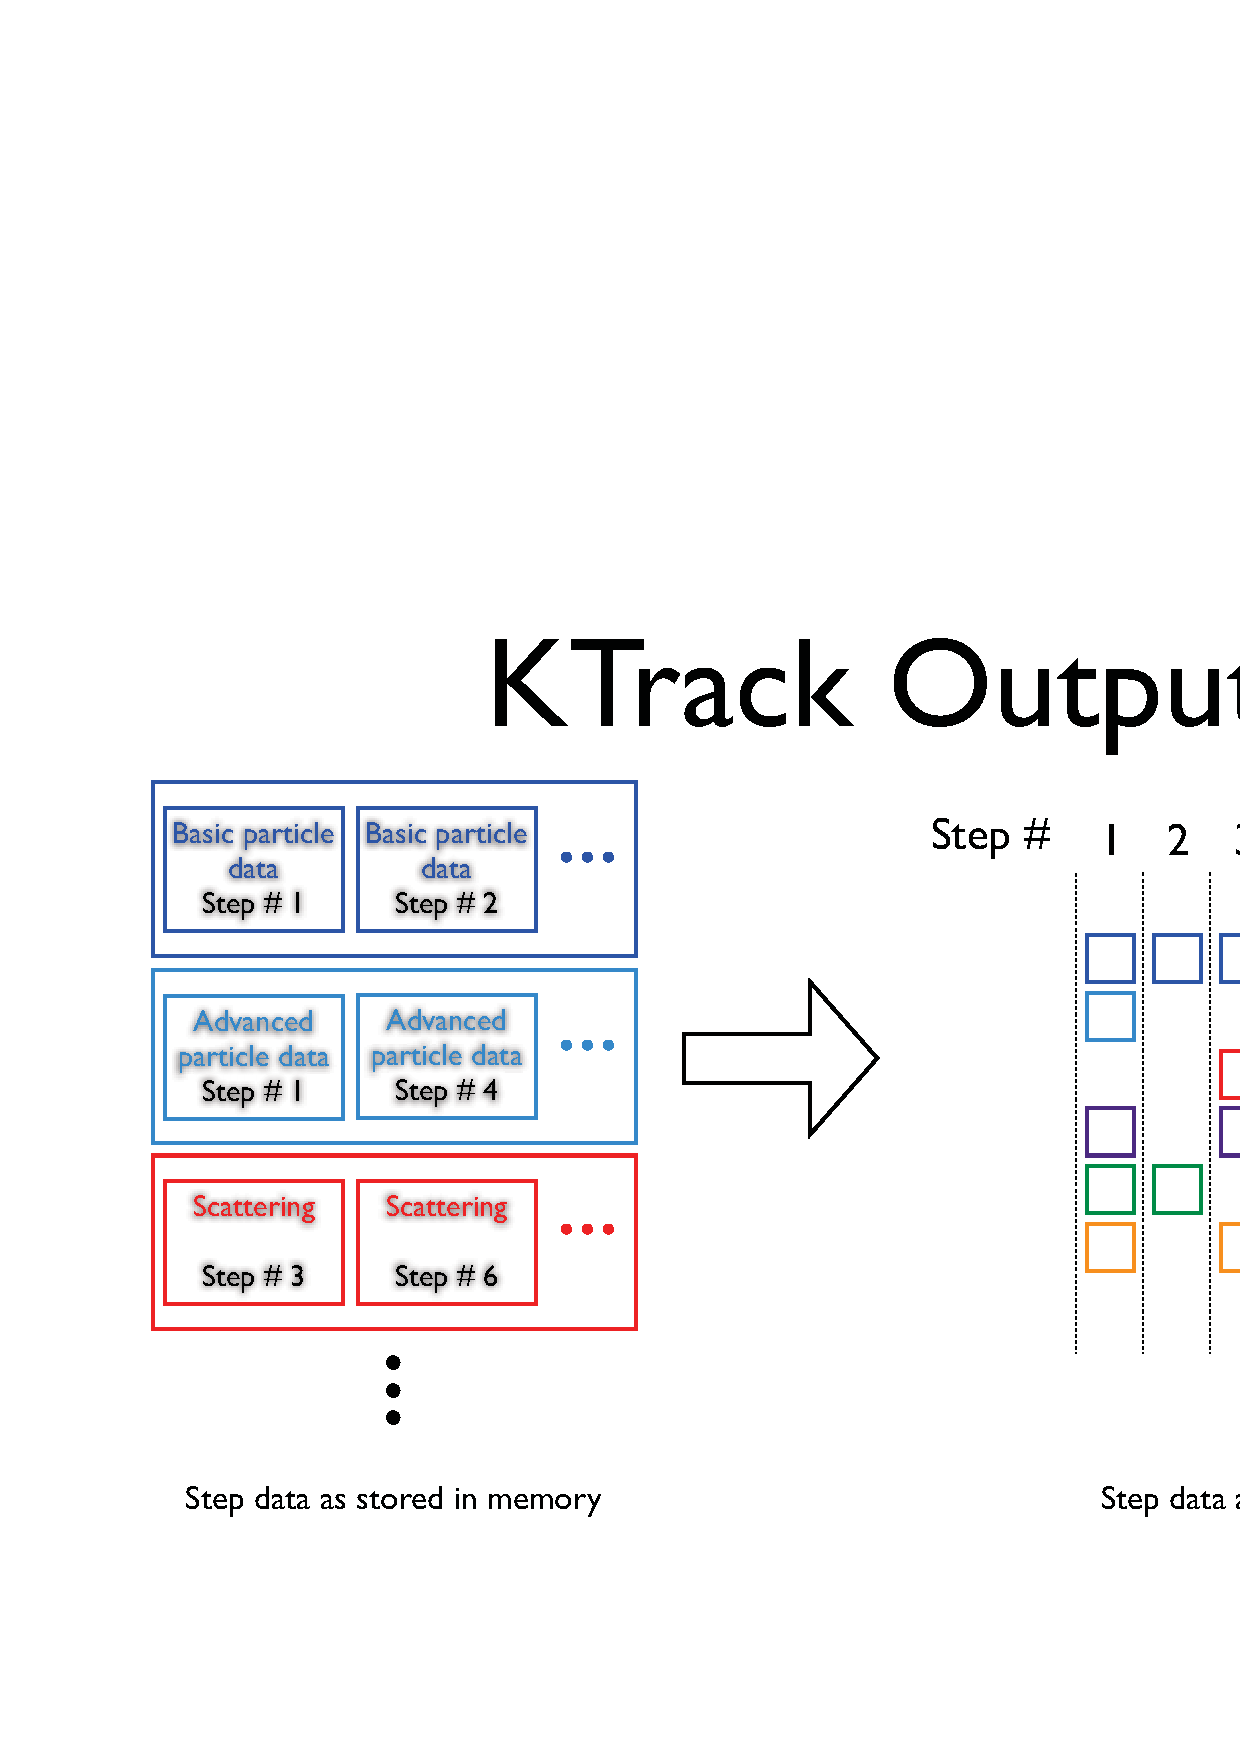
\includegraphics[width=\textwidth]{images/Output_fig2}
\caption{Step Keys scheme}
\end{DoxyImage}
 


\begin{DoxyImage}
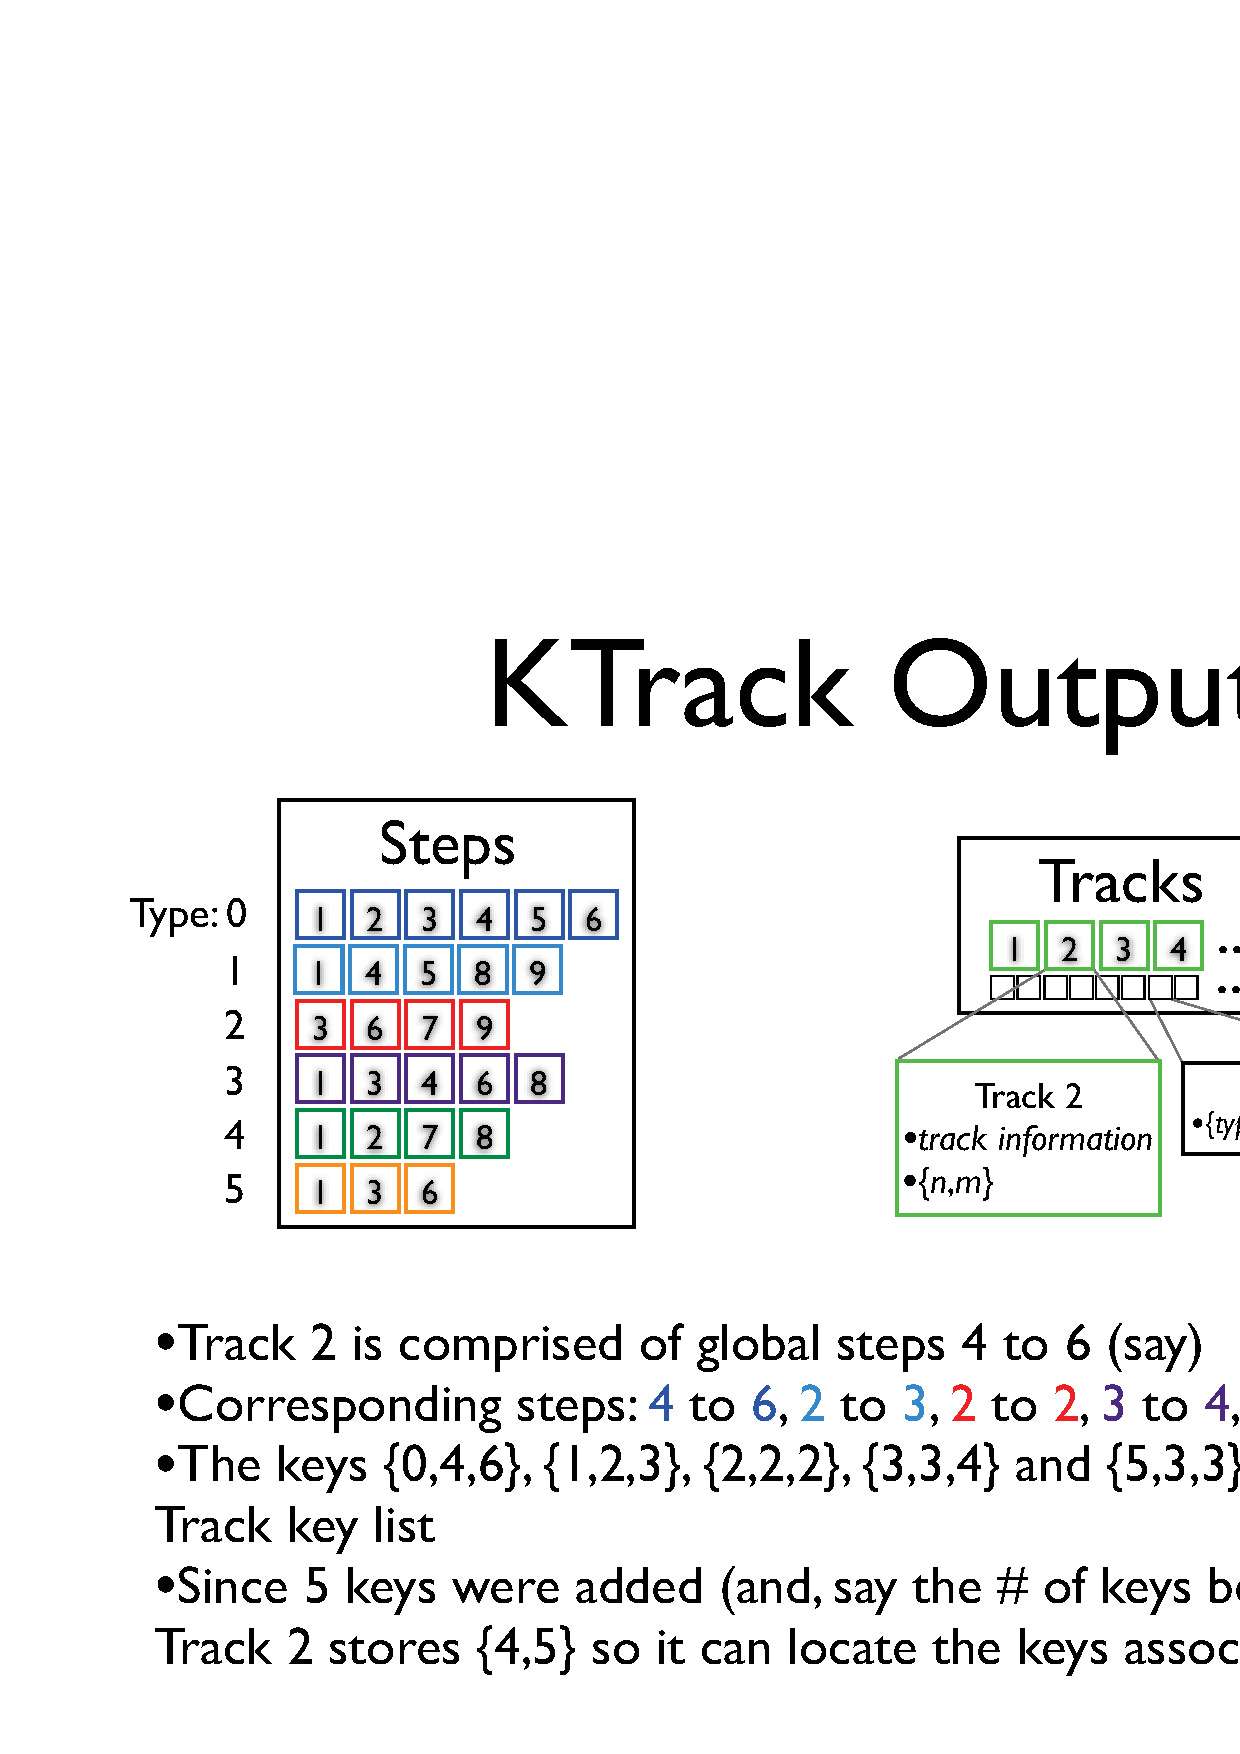
\includegraphics[width=\textwidth]{images/Output_fig3}
\caption{Step Keys example}
\end{DoxyImage}
 

In order to ensure accessibility of the data at all times, the output classes have a version ID provided by the \hyperlink{namespace_r_o_o_t}{ROOT} object IO system. If their design changes, this version number will have to be increased.\hypertarget{_k_s_output_KSAnalysis}{}\subsection{Analysis}\label{_k_s_output_KSAnalysis}


 \hypertarget{_k_s_output_KSTools}{}\subsubsection{existing tools}\label{_k_s_output_KSTools}
As an extremely preliminary general analysis tool, the macro FileReader.C is installed in the binary folder. It can be used as follows: First of all, start root. Then in root do: 
\begin{DoxyCode}
      root [0] .L /path/to/kassiopeia/bin/FileReader.C
      root [1]  FileReader("/path/to/filename", "/path/to/kassiopeia/lib);
\end{DoxyCode}
 The intension of that macro is that the user adjusts it to suite his purposes. That is the main reason why it is provided as a \hyperlink{namespace_r_o_o_t}{ROOT} macro, not a compiled binary. Apart from missing header inclusions, the code in the macro compiles. So if you want to compile your own analysis code, the following piece of code shows how to read the output. It is a one to one copy from the macro FileReader.C. Make sure to read the section about linking to kassiopeia. This code works regardless of the file format, although it is to some extend experimental. Note that the the Filereader macro gets overwritten everytime you do make install, so you better rename it. It's original source code can be found in Application/Macros...


\begin{DoxyCode}
  Kassiopeia::KMCDataManager* myManager = 
      Kassiopeia::KMCDataManager::GetInstance();
  myManager->OpenFile(argv[1],0);
  Kassiopeia::KMCEventIterator* myevent2 = myManager->GetEvent();
  //unitilized pointer to event data, does not contain any useful information at 
      this point

  for (UInt_t ievent = 0; ievent < myManager->GetNEvents(); ievent++){
      myManager->ReadNextEvent(); //now we load the event data of the next event.
      
      Kassiopeia::KMCTrackIterator* mytrack2 = myevent2->GetTrack();
      for (UInt_t itrack = 0; itrack < myevent2->GetNTracks(); itrack++){
          myevent2->ReadNextTrack();
          Kassiopeia::KMCStepIterator* myStep2 = mytrack2->GetStep();
          for (UInt_t istep = 0; istep < mytrack2->GetNSteps(); istep++){
              mytrack2->ReadNextStep();
          }
      }
  }
\end{DoxyCode}
 Additionally, a program called Trackplotter is installed, which plots the geometry and tracks of a simulation.\hypertarget{_k_s_output_KSlinking}{}\subsubsection{Linking}\label{_k_s_output_KSlinking}
In case you want to link your own code against kassiopeia, you can use the 'pkg-\/config'utility to print the compiler and linker flags using 
\begin{DoxyCode}
 pkg-config --cflags kassiopeia
 pkg-config --libs kassiopeia
\end{DoxyCode}
 in the command line or rather your makefile. pkg-\/config is a general tool, its purpose is similar to the root-\/config utlity you probably know. The way this works is that \hyperlink{class_kassiopeia}{Kassiopeia} installs a file called libkassiopeia.pc. This file tells pkg-\/config the necessary information so that it can print the linker options. For this to work, pkg-\/config must find this file! That either requires that you install kassiopeia in a default place like /usr/, or that you add the directory containing kassiopeia.pc (@/@/pkg-\/config) to the environment variable PKG\_\-CONFIG\_\-PATH.\hypertarget{_k_s_output_KSdynamicLoading}{}\subsubsection{Dynamic loading of kassiopeias output classes in ROOT}\label{_k_s_output_KSdynamicLoading}
Another small little feature which might come in handy: \hyperlink{class_kassiopeia}{Kassiopeia} installs a file called libkassiopeia.rootmap. This file tells root in a CINT session (i.e. the root command line), which libraries it needs to load if it encounters kassiopeias classnames. CINT will then try to do that. Of course it only works, if root finds the rootmap file and the library. I haven't found any explicit documentation where \hyperlink{namespace_r_o_o_t}{ROOT} searches for these files, but it seems to look for bith in the current directory, default places like /usr/lib, the root library directory probably LD\_\-LIBRARYPATH.

You can check whether \hyperlink{namespace_r_o_o_t}{ROOT} knows the kassiopeia DataStructure classes by opening a simulation output file in root, e.g. by passing it as argument to root, when starting it. in that case, you could directly use 
\begin{DoxyCode}
    Kassiopeia::KMCDataManager* myManager = 
      Kassiopeia::KMCDataManager::GetInstance();
\end{DoxyCode}
 and the following lines from the block above, in a CIONT session and it would work...

if you see lots of warnings like that, 
\begin{DoxyCode}
Warning in <TClass::TClass>: no dictionary for class Kassiopeia::KMCEventData is 
      available
...
\end{DoxyCode}
 \hyperlink{namespace_r_o_o_t}{ROOT} has not found the rootmap file. If you additionally see 
\begin{DoxyCode}
Warning in <TClass::TClass>: no dictionary for class Kassiopeia::KMCEventData is 
      available
Error in <TUnixSystem::DynamicPathName>: libKSDataStructure.so does not exist in 
      .:...
...
\end{DoxyCode}
 \hyperlink{namespace_r_o_o_t}{ROOT} has found the rootmap file, but not the library.

and if it just opens the file without any complaints, everything works. Congratulations.

The filereader macro does not rely on the correct installation of the rootmap file, but rather forces the user to specify the directory of the library by hand. 


% Programming guide for the Kassiopeia Guide
\chapter{Modules}\label{sec:modules}\label{ch:modules}

The modules in Kassiopeia include all of the tools that go in the toolboxes.  They are categorized based on their purpose within Kassiopeia.  The modules are:

\flushleft
\begin{description}
\item[Field Calculators]\quad
	\begin{itemize}
	\item KAFCA -- Ferenc's Field Simulation
	\item KNAXS -- Non-Axially-Symmetric Field Simulation
	\item KEMField -- Comprehensive Field Simulation
	\end{itemize}
\item[Generators]\quad
	\begin{itemize}
	\item KPAGE -- KATRIN PArticle GEnerator
	\end{itemize}
\item[Tracking]\quad
	\begin{itemize}
	\item KTrack -- General Particle Tracking
	\item KESS -- KATRIN Electron Scattering in Silicon
	\end{itemize}
\item[Tritium Source]\quad
	\begin{itemize}
	\item{SSC} -- Source Spectrum Calculation
	\end{itemize}
\item[Data Acquisition]\quad
	\begin{itemize}
	\item{DAQ}
	\end{itemize}
\end{description}


% KAFCA documentation for the Kassiopeia Guide
% B.Leiber email: benjamin.leiber@kit.edu
\section{Ferenc's Field Simulation: KAFCA}\label{sec:KAFCA}
\subsection{Magnetic field calculation with the Legendre polynomial expansion}
%% =============================
	\subsubsection{Elliptic Integrals}
	  The main components generating magnetic fields in the KATRIN experiment are circular coils and superconducting solenoids. These are simple circular current loops, that have a rotational symmetry axis (compare fig. \ref{fig:current loop}). 
	  \begin{figure}[h]
		\centering 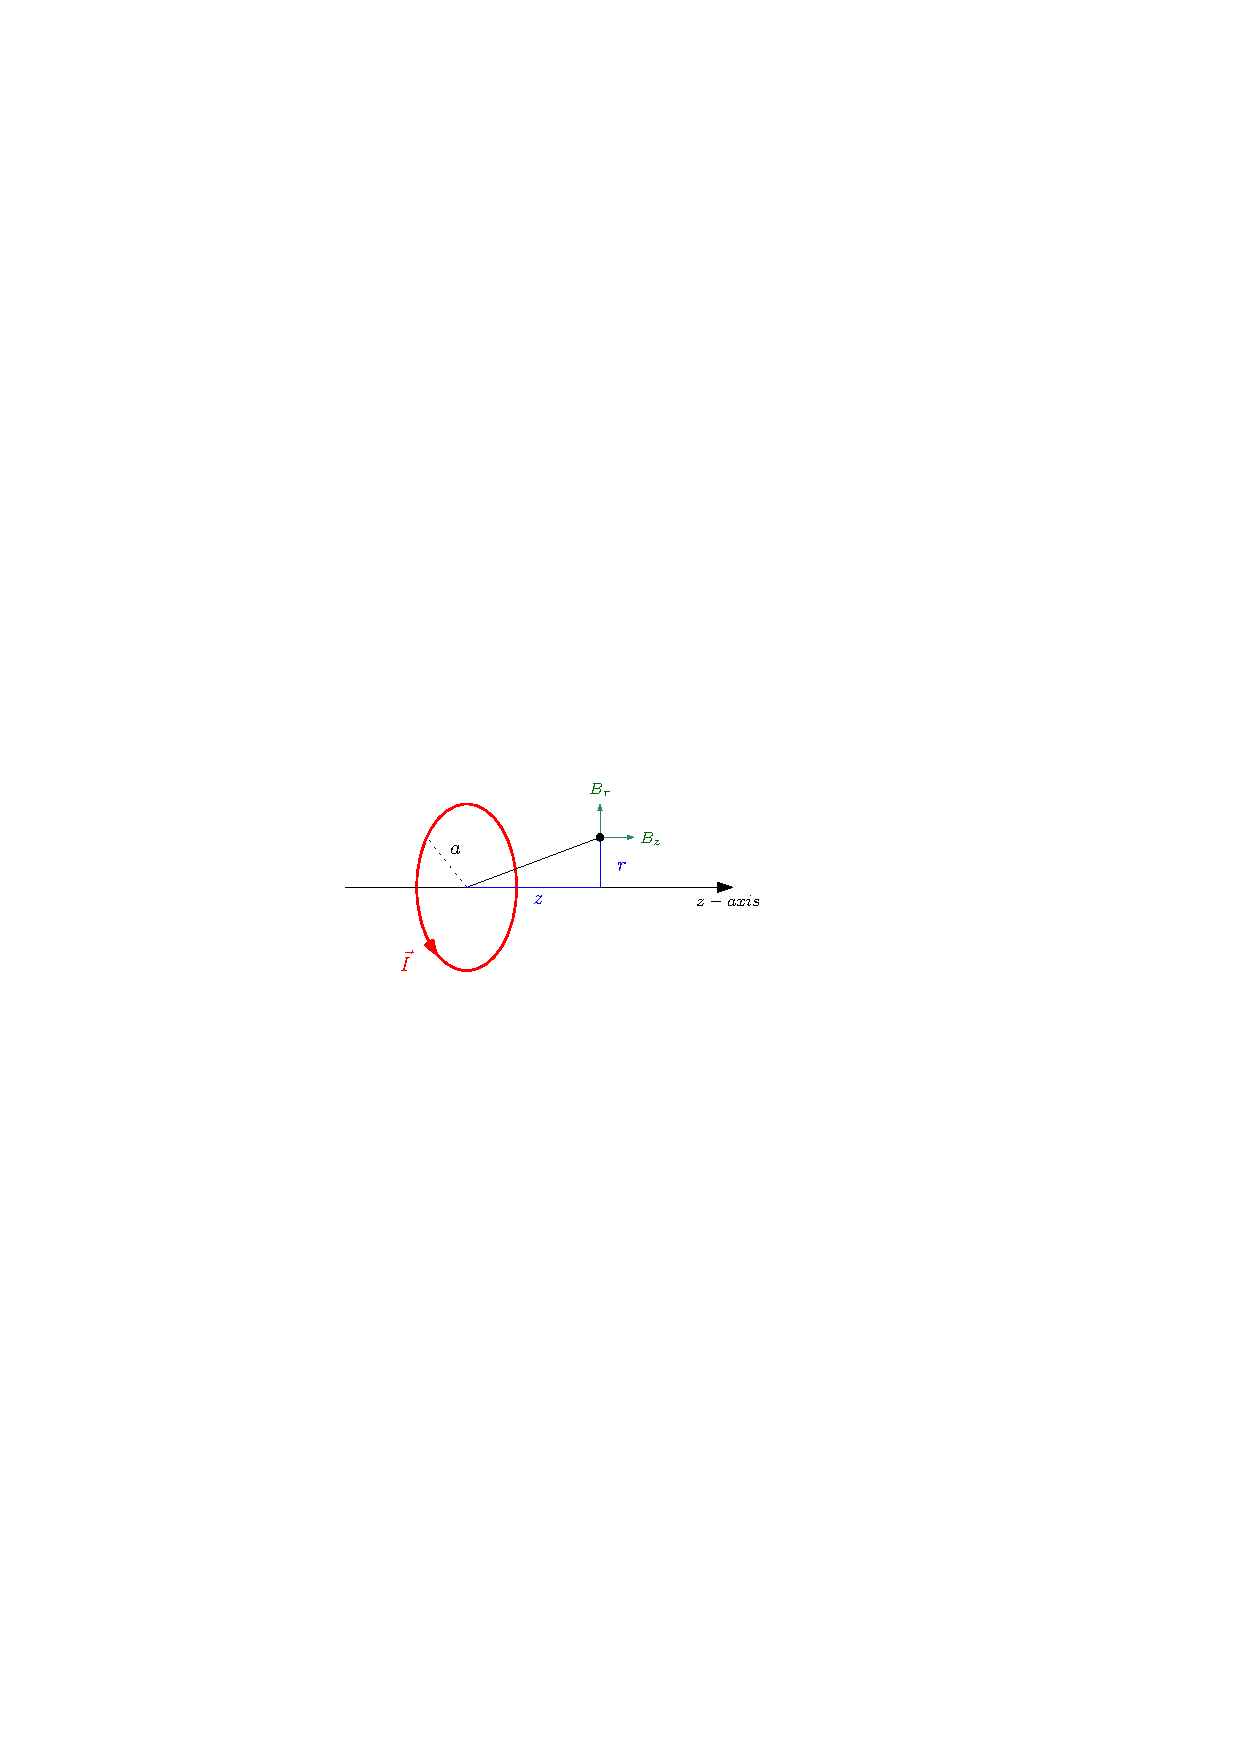
\includegraphics[width=0.7\textwidth]{images/KAFCAFigures/current_loop.pdf}
		\caption{A loop with the radius $a$ and the current $\vec{I}$ running through it, induces a magnetic field $\vec{B}$}
		\label{fig:current loop}
	  \end{figure}\\
	  The Biot-Savart law \eqref{eq:biot savart} for a thin coil can be expressed in terms of the complete elliptic integrals:
%====================	
	%elliptic Integrals
	\begin{equation}
		\begin{aligned}
			K(k) &= \int\limits_{0}^{\frac{\pi}{2}} \frac{\mathrm d\varphi}{\sqrt{1-k^{2}\sin^{2}\varphi}} & \text{(I)}\\
			E(k) &= \int\limits_{0}^{\frac{\pi}{2}} \mathrm{d}\varphi\sqrt{1-k^{2}\sin^{2}\varphi} & \text{(II)} \\
			\Pi(c,k) &= \int\limits_{0}^{\frac{\pi}{2}} \frac{\mathrm d\varphi}{(1-c^{2}\sin^{2}\varphi)\sqrt{1-k^{2}\sin^{2}\varphi}}  & \text{(III)}
		\end{aligned}
		\label{eq:complete elliptic integrals}
	\end{equation}
	They can be used for an analytical computation of the magnetic field \cite{jackson}:
	\begin{equation}
		\begin{aligned}
			B_{r} &= \frac{I}{c} \frac{2z}{r\sqrt{(a+r)^{2}+z^{2}}} \left[ -K(k) + \frac{a^{2}+r^{2}+z^{2}}{(a+r)^{2}+z^{2}}E(k)\right] \\
			B_{\varphi} &= 0 \\
			B_{z} &= \frac{I}{c} \frac{2}{r\sqrt{(a+r)^{2}+z^{2}}} \left[ K(k) + \frac{a^{2}-r^{2}-z^{2}}{(a+r)^{2}+z^{2}}E(k)\right]
		\end{aligned}
		\label{eq:magnetic field elliptic integrals}
	\end{equation}
	where $k^2 = \frac{4ar}{z^2 + \left(a+r\right)^2}$. For real coils, with a finite length, the third integral is also needed for a description of the magnetic field. Usually, $K(k)$, $E(k)$ and $\Pi(c,k)$ are expressed via Carlson's elliptic integrals $R_F$, $R_J$, $R_D$ \cite{numericalrecipes}: 
	\begin{equation}
		\begin{aligned}
			K(k) &= (R_{F},0, 1-k^{2},1)\\
			E(k) &= (R_{F},0, 1-k^{2},1) - k^{2}\frac{1}{3}(R_{D},0, 1-k^{2},1) \\
			\Pi(c,k) &= (R_{F},0, 1-k^{2},1) - c^{2}\frac{1}{3}(R_{J},0, 1-k^{2},1,1-c^{2})
		\end{aligned}
		\label{eq:complete elliptic integrals through carlson}
	\end{equation}
	These solutions are valid everywhere and hence, the magnetic field can even be calculated inside the coils. In addition, Carlson's elliptic integrals offer a relatively fast numerical computation method. But still a numerical integration is necessary, which usually means summing over many numbers. To speed things up, a solution has to be found that is fast to compute: the zonal-harmonics are appropriate solutions for axisymmetric coils. They can be computed fast and offer a variable precision, depending on the number of expansion orders that are considered.
      \subsubsection{Zonal Harmonic Expansion}
	The magnetic field at a point $\vec{p}(r,z)$ close to the symmetry axis, can be expressed in terms of the Legendre polynomial expansion and its derivatives at the point $z_0$ that lies on the symmetry axis, a so called sourcepoint. In case the distance of the field-point to the sourcepoint is smaller than the minimal distance of the sourcepoint to the coil body ($\rho < \rho_{cen}$, see fig. \ref{fig:central convergence radius}), the magnetic field is given by the so called central expansion:
	\begin{equation}
		\begin{aligned}
			B_r &= -s\sum_{n=1}^{\infty} \frac{B_{n}^{cen}}{n+1} \left(\frac{\rho}{\rho_{cen}}\right)^{n}P'_n(u) \\
			B_{\varphi} &= 0 \\
			B_z &= \sum_{n=0}^{\infty} B_{n}^{cen}\left(\frac{\rho}{\rho_{cen}}\right)^{n}P_n(u) \\
			&\text{with} \quad u = \cos\theta \quad \text{and} \quad s = \sin\theta
		\end{aligned}
		\label{eq:central polynomial expansion}
	\end{equation}
	with $B_{n}^{cen}$ being the central source coefficients and $P_{n}$ the Legendre polynomials. The minimal distance between the sourcepoint and the coil $\rho_{cen}$ is usually called central convergence radius and equation \eqref{eq:central polynomial expansion} is only valid within.
	  \begin{figure}[h]
		\centering 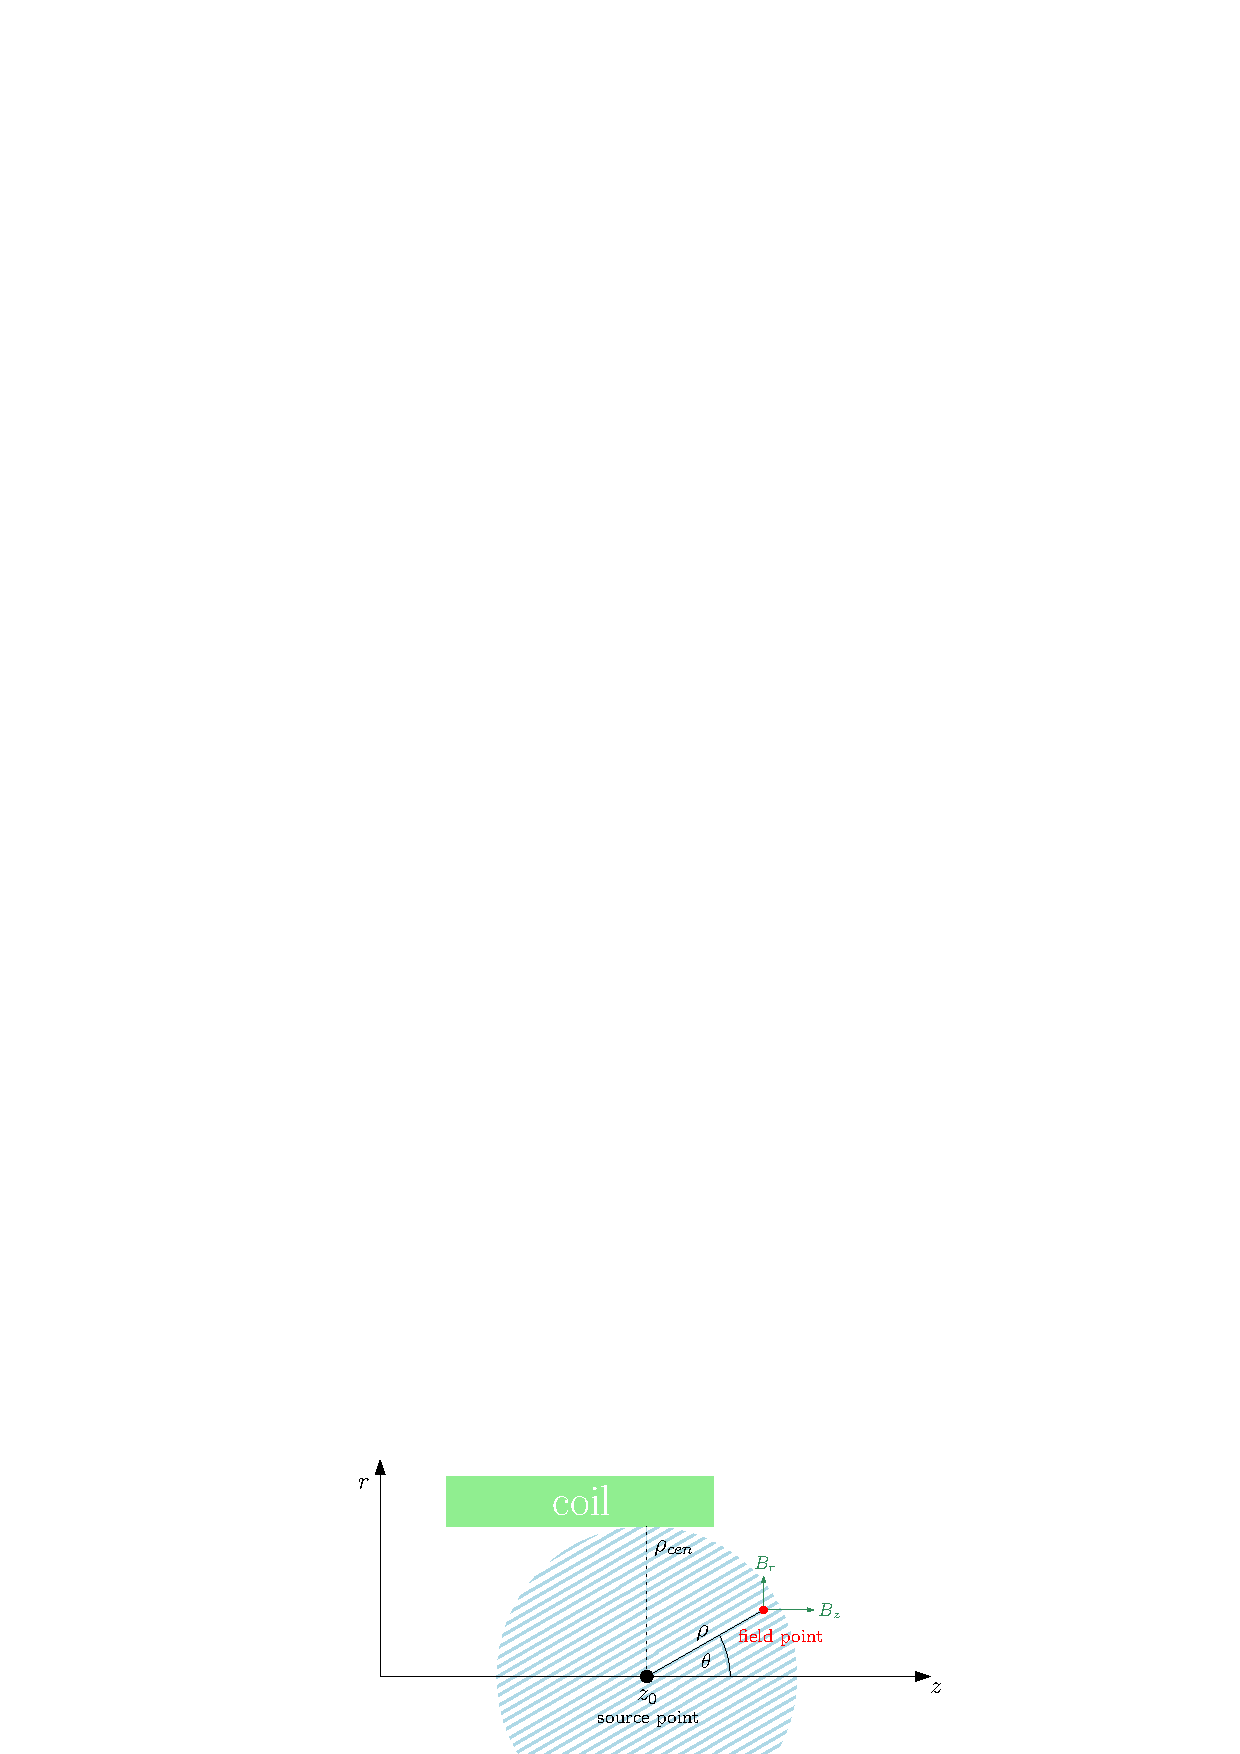
\includegraphics[width=0.7\textwidth]{images/KAFCAFigures/legendre_central.pdf}
		\caption{Convergence radius of the central expansion.}
		\label{fig:central convergence radius}
	  \end{figure}
	  \\
	As we want to know the magnetic field outside of the convergence radius too, a second polynomial expansion has to be introduced. This remote expansion is only valid for distances to the sourcepoint greater than the remote convergence radius $\rho_{rem}$, which is the maximal distance of the sourcepoint to the coil ($\rho > \rho_{rem}$, see fig. \ref{fig:remote convergence radius}). The magnetic field is then defined by the remote expansion:
	\begin{equation}
		\begin{aligned}
			B_r &= s\sum_{n=2}^{\infty} \frac{B_{n}^{rem}}{n} \left(\frac{\rho_{rem}}{\rho}\right)^{n+1}P'_n(u) \\
			B_{\varphi} &= 0 \\
			B_z &= \sum_{n=2}^{\infty} B_{n}^{rem}\left(\frac{\rho_{rem}}{\rho}\right)^{n+1}P_n(u) %\\
			%&\text{with} \quad u = \cos\theta \quad \text{and} \quad s = \sin\theta
		\end{aligned}
		\label{eq:remote polynomial expansion}
	\end{equation}
	with $B_{n}^{rem}$ being the remote source coefficients.
	\begin{figure}[h]
		\centering 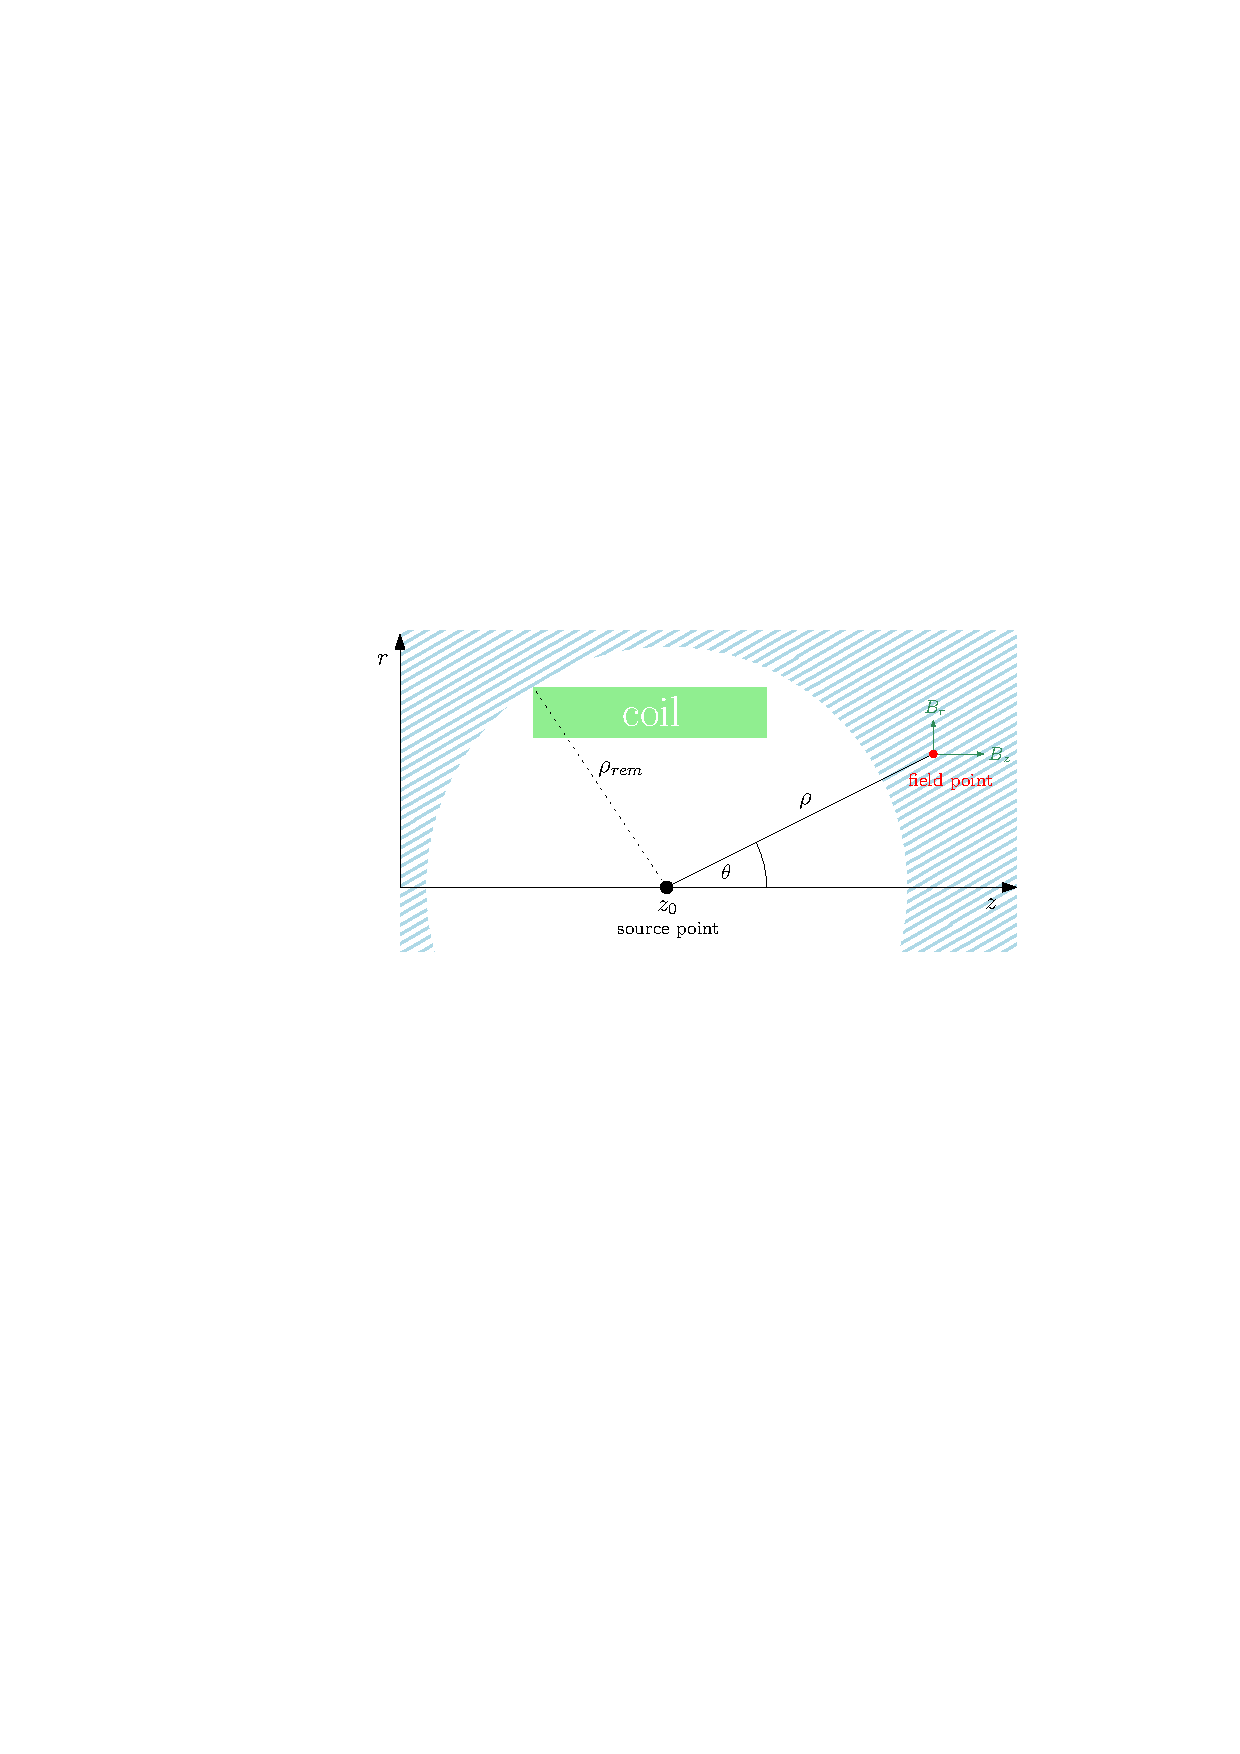
\includegraphics[width=0.7\textwidth]{images/KAFCAFigures/legendre_remote.pdf}
		\caption{Convergence radius of the remote expansion.}
	  \label{fig:remote convergence radius}
	\end{figure}
	\\
	These expansions now allow a very fast field-computation nearly everywhere in the system. They are not valid close to and inside the coils, so elliptic integrals have to be used here.
      %\subsubsection{Implementation}
      \subsubsection{Application}
	For the description of a system of multiple coils, the convergence radii are determined by the closest, respectively the most remote coil (see fig. \ref{fig:two coils one sourcepoint}).
	\begin{figure}[htbp]
	      \centering
	      %\begin{minipage}{0.7\textwidth}
	      \begin{minipage}{0.49\textwidth}
		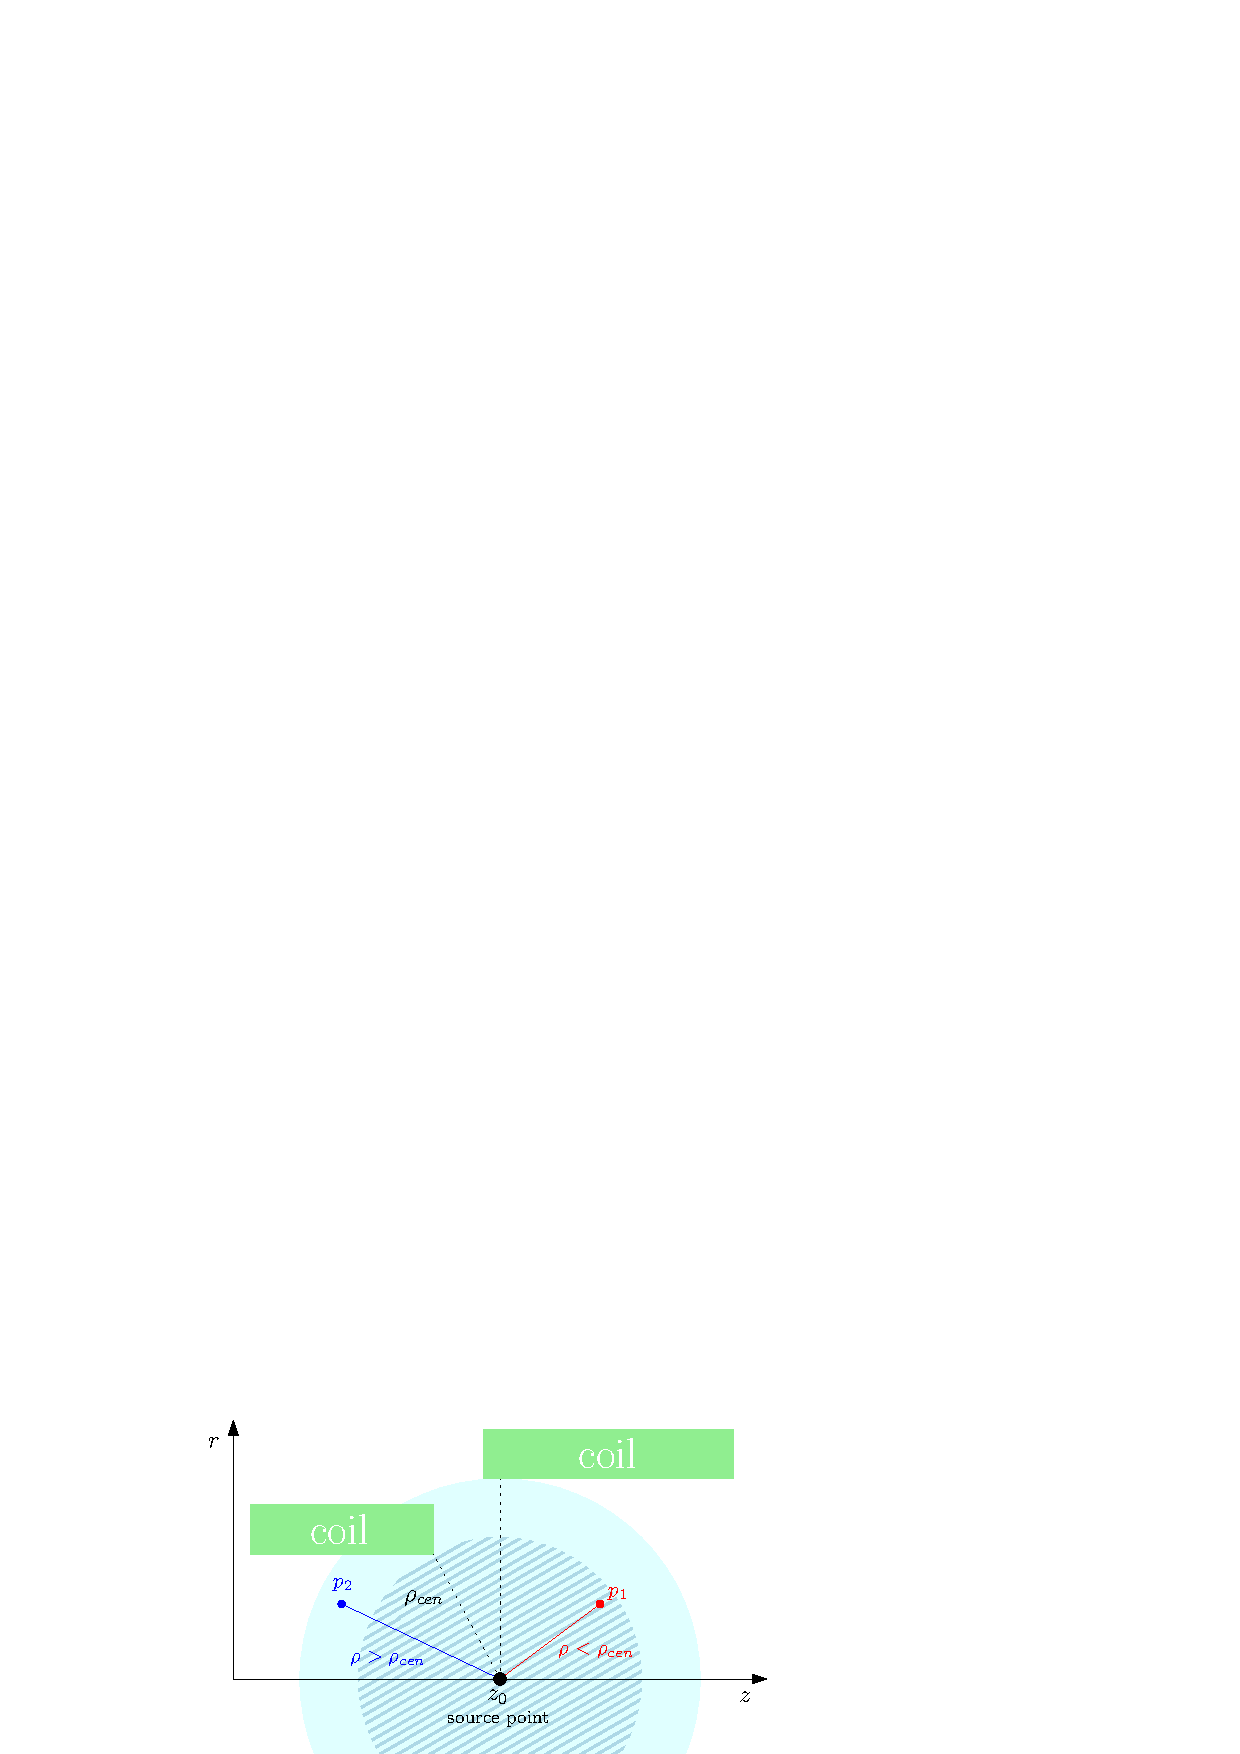
\includegraphics[width=0.95\textwidth]{images/KAFCAFigures/two_coils_central.pdf}
	      \end{minipage}
	      %\\
	      %\begin{minipage}{0.85\textwidth}
	      \begin{minipage}{0.49\textwidth}
		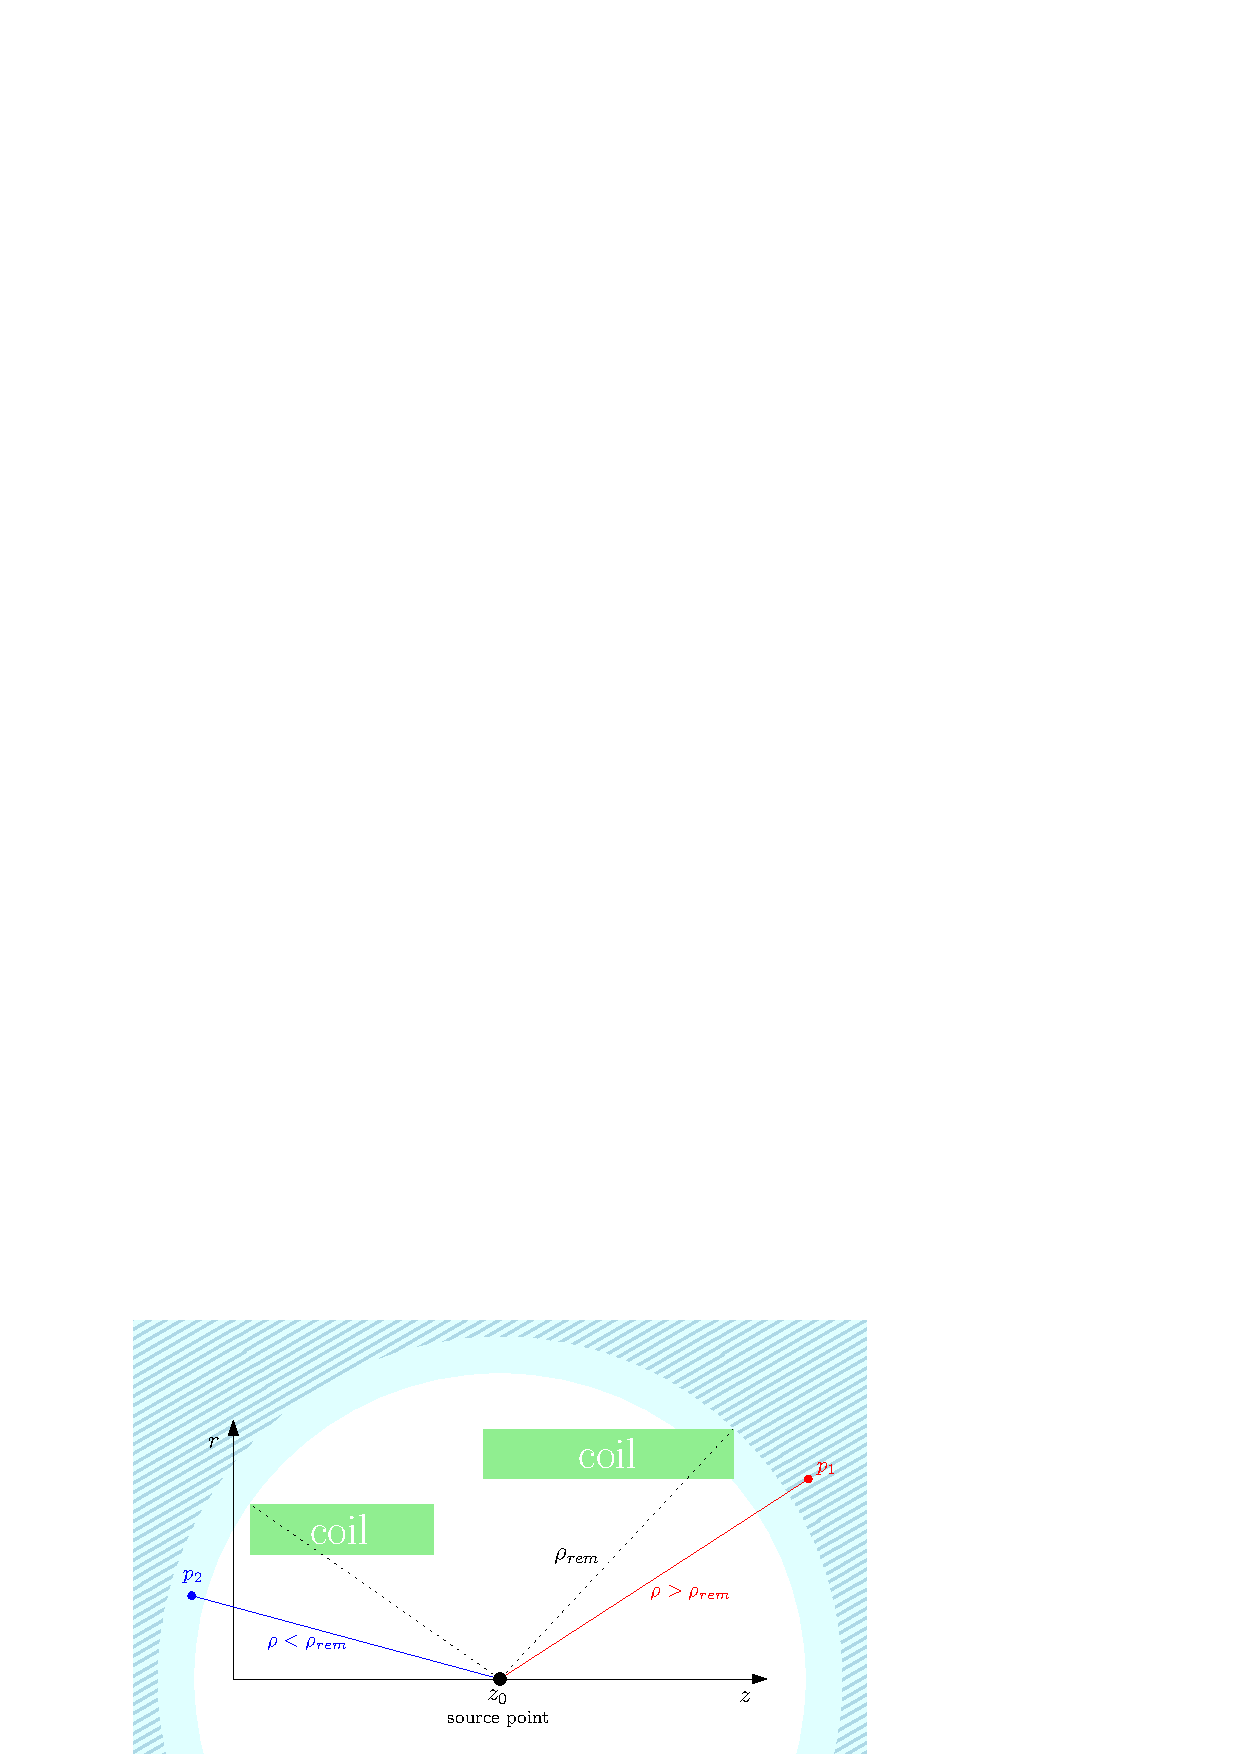
\includegraphics[width=0.95\textwidth]{images/KAFCAFigures/two_coils_remote.pdf}
	      \end{minipage}
	      \caption{Central convergence radius (top) and remote convergence radius (below), with two coils using only one sourcepoint. The expansions converge in $p_1$ but not in $p_2$.}
	      \label{fig:two coils one sourcepoint}
	\end{figure}
	To cover a larger area the amount of sourcepoints can simply be increased as shown in figure\ref{fig:two coils two sourcepoints}.
	\begin{figure}[htbp]
	      \centering
	      %\begin{minipage}{0.7\textwidth}
	      \begin{minipage}{0.49\textwidth}
		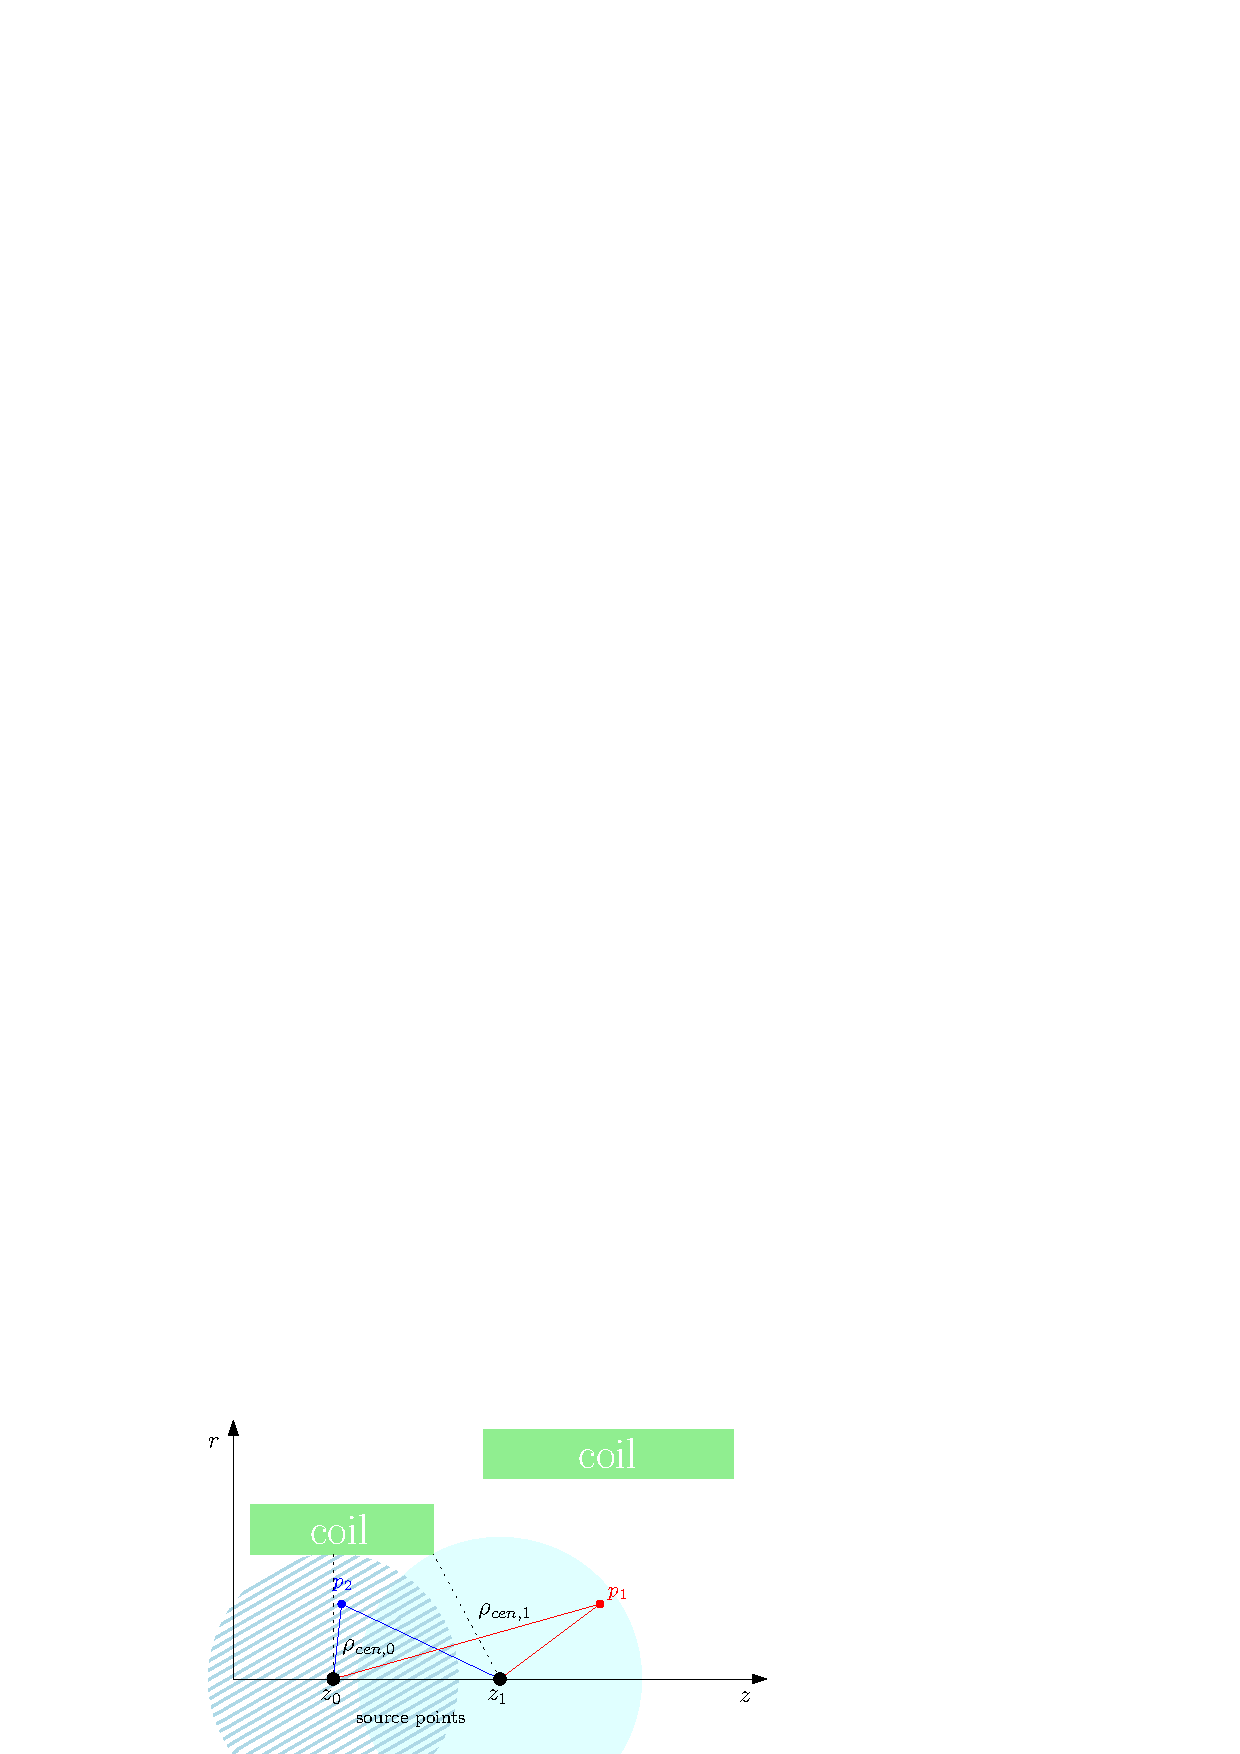
\includegraphics[width=0.95\textwidth]{images/KAFCAFigures/two_coils_central_two_sp.pdf}
	      \end{minipage}
	      %\\
	      %\begin{minipage}{0.85\textwidth}
	      \begin{minipage}{0.49\textwidth}
		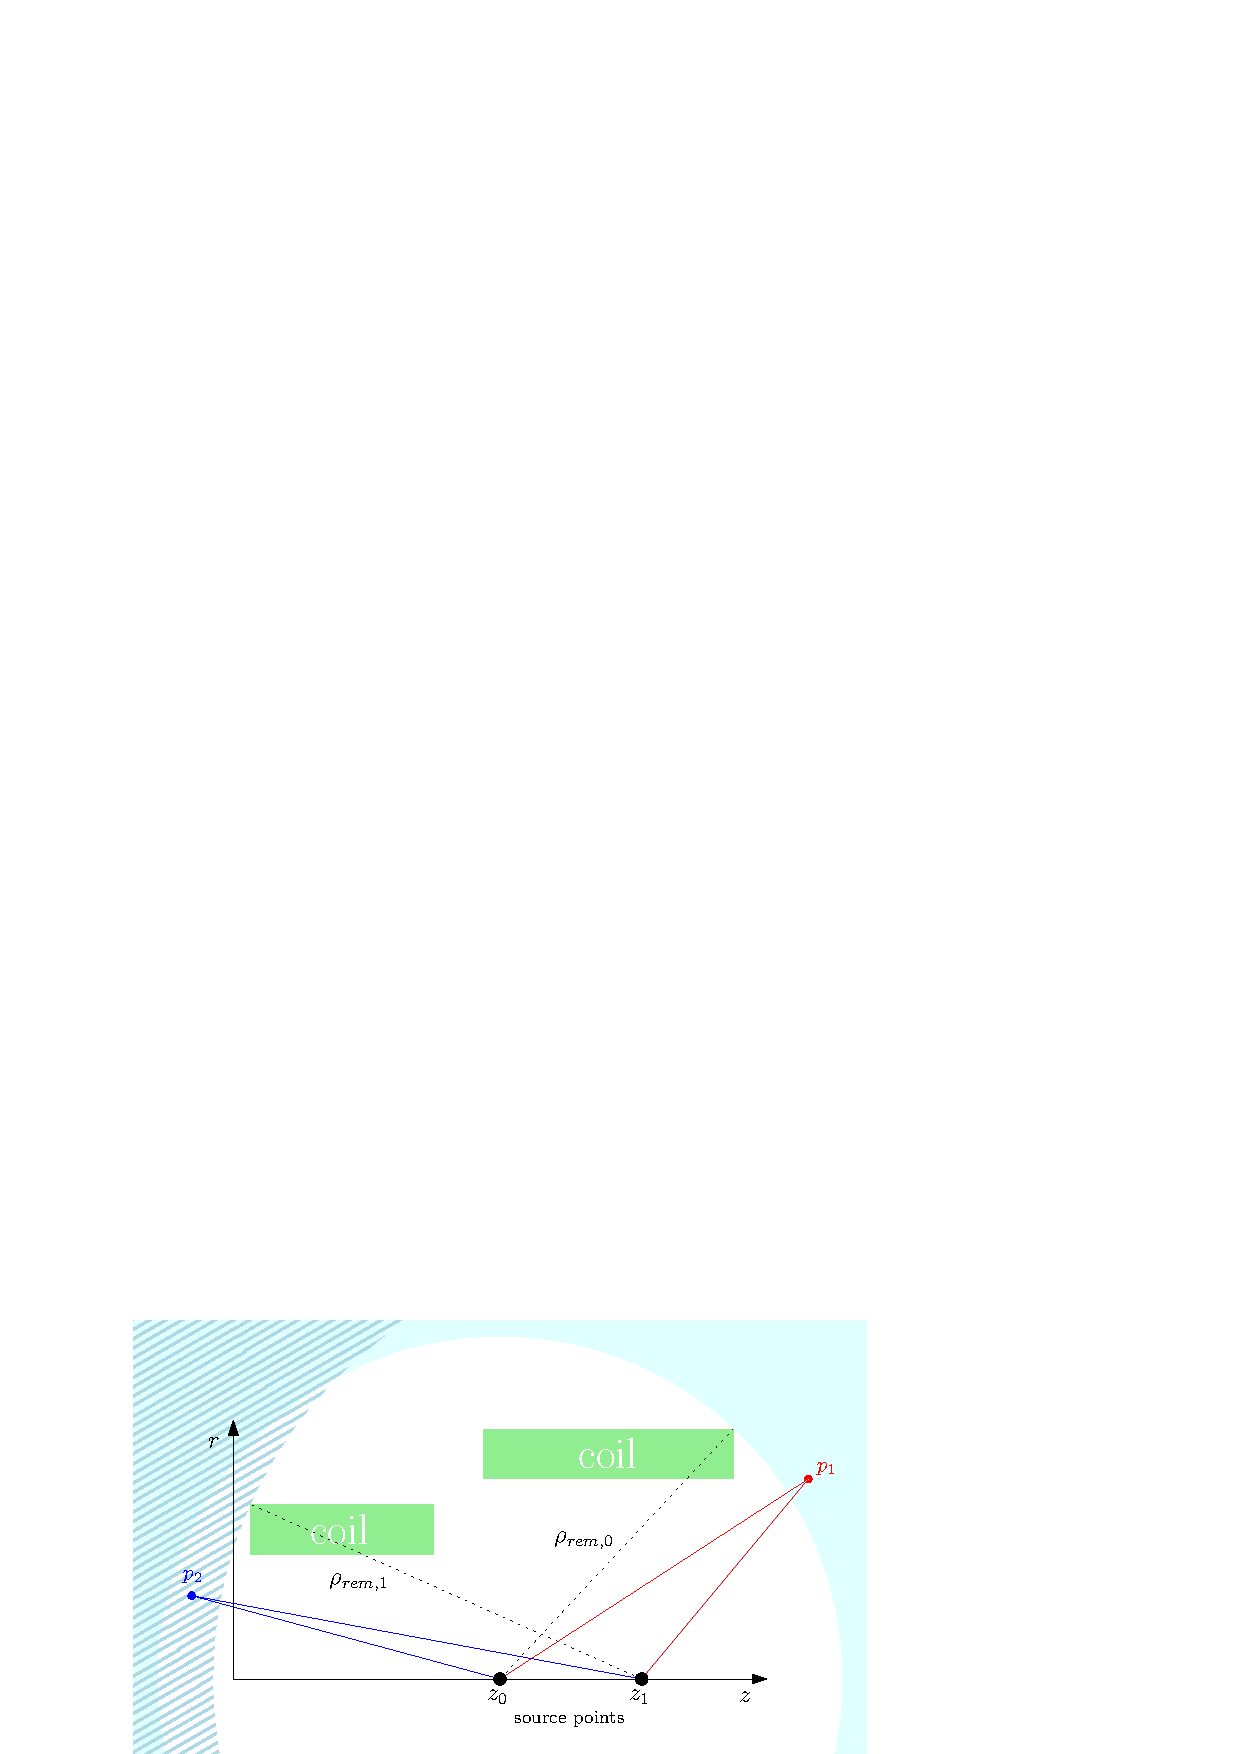
\includegraphics[width=0.95\textwidth]{images/KAFCAFigures/two_coils_remote_two_sp.pdf}
	      \end{minipage}
	      \caption{With the additional sourcepoints, it is now possible to compute the magnetic field in both $p_1$ and $p_2$ with the polynomial expansion.}
	      \label{fig:two coils two sourcepoints}
	\end{figure}
	Another benefit of having several sourcepoints is a faster computation, as the polynomial expansion converges faster if the fractions $\frac{\rho}{\rho_{cen}}$ and $\frac{\rho_{rem}}{\rho}$ are smaller. By choosing the sourcepoint with the smallest fraction for the field point to be calculated, a lot of computation time can be saved.
	\\
	In preparation for the polynomial expansion, the source coefficients $B_{n}^{cen}$ and $B_{n}^{rem}$ need to be computed at every sourcepoint. They can be expressed in two dimensional integrals over the coil profile:
	\begin{equation}
		\begin{aligned}
			B_{n}^{cen} &= \int\limits_{R_{min}}^{R_{max}} \mathrm{d}R \int\limits_{Z_{min}}^{Z_{max}} \mathrm{d}Z ~b_{n}(R,Z) \quad\text{and}  \\
			B_{n}^{rem} &= \int\limits_{R_{min}}^{R_{max}} \mathrm{d}R \int\limits_{Z_{min}}^{Z_{max}} \mathrm{d}Z ~b_{n}^{*}(R,Z)\text{,}
		\end{aligned}
		\label{eq:source coefficients integrals}
	\end{equation}
	with
	\begin{equation}
		\begin{aligned}
			b_{n}(R,Z) &= \frac{\mu_{0}I}{2A\rho_{cen}} \left( 1 - \left(\frac{Z-z_0}{\rho_{ZR}}\right)^{2}\right)\left(\frac{\rho_{cen}}{\rho_{ZR}}\right)^{n+1} P'_{n+1}\left(\frac{Z-z_0}{\rho_{ZR}}\right) \text{,}  \\
			b_{n}^{*}(R,Z) &= \frac{\mu_{0}I}{2A\rho_{rem}} \left( 1 - \left(\frac{Z-z_0}{\rho_{ZR}}\right)^{2}\right)\left(\frac{\rho_{rem}}{\rho_{ZR}}\right)^{n} P'_{n-1}\left(\frac{Z-z_0}{\rho_{ZR}}\right)\text{,}
		\end{aligned}
		\label{eq:source coefficients}
	\end{equation}
	$\rho_{ZR}$ being the distance between the sourcepoint $z_0$ and the point $(Z,R)$ in the coil body and $\frac{I}{A}$ being the current density within the coil. 
	\\ 
	It is even possible to compute the field of multiple coils that do not have a common symmetry axis. In this case, the coils can be merged into groups with common symmetry axes (see fig. \ref{fig:tilted coils}). The source coefficients are computed for the sourcepoints in the respective coordinate system. Afterwards the magnetic field is transformed back into the reference system.
	\begin{figure}[h]
		\centering 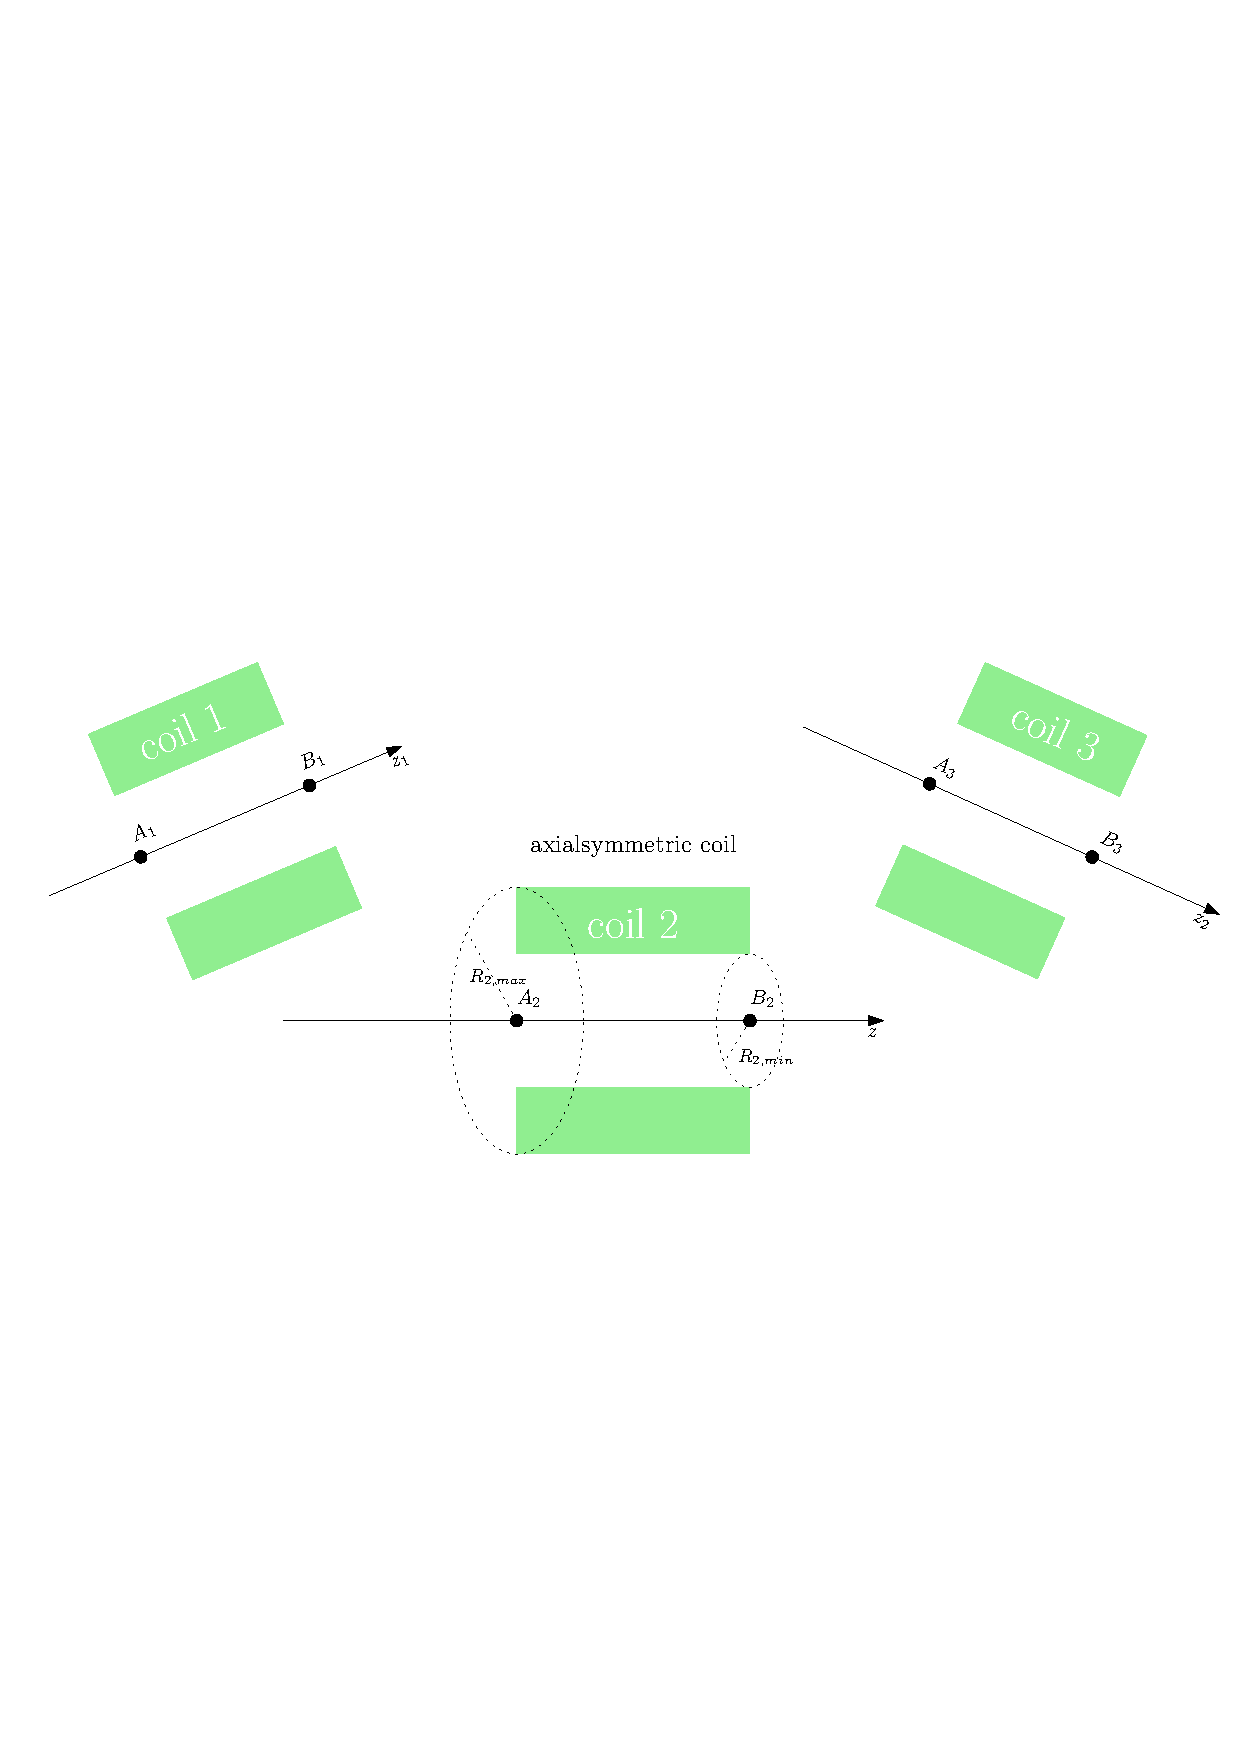
\includegraphics[width=1.0\textwidth]{images/KAFCAFigures/tilted_coils.pdf}
		\caption{Tilted coils with different symmetry axes}
	  \label{fig:tilted coils}
	\end{figure}
%% =============================
%% =============================
%% =============================
%
%
%
\subsection{Electric field calculation}
\label{ch:Methods for electric and magnetic field-calculation:sec:Electric field calculation}
  Electric field and potential calculations turn out to be more complicated than the magnetic ones. Magnetic fields are caused by electric current, a quantity which can be directly measured and set. The electric field and potential, however,  are caused by a charge distribution that is usually not known. The quantity you can set and measure on your electrodes is the voltage. The charge density on the electrodes is dependent on the voltage, but also highly dependent on the geometry of the electrode itself and on its surrounding. Another KATRIN-specific requirement is the ability to handle large volumes enclosed by electrodes. Most of the methods used to simulate electric fields, like for example the Finite Difference Method, are not applicable in such a case, as they divide the volume into a close-meshed grid, which, for extended geometries, can not be handled without serious problems regarding computer memory. \\
  Actually, a method exists that meets these requirements, the so called \textbf{B}oundary \textbf{E}lement \textbf{M}ethod.
%% =============================
	\subsection{Boundary element method}
	  Working with the boundary element method (BEM), it is assumed that on a given surface-part of the electrode the charge density is distributed homogeneously and the resulting electric field can be derived from it. Analogous to the line-segment methods discussed earlier in this chapter, the discretization into surface elements offers the ability to form any complex shape out of such elements with variable level of detail and thereby accuracy.\\
	  An electrode can be discretized into $N$ sub-elements $S_j$. The geometry $S$ can be written as a sum of these sub-elements:
	\begin{equation}
		S = \sum_{j=1}^{N} S_j
		\label{eq:sum over geometry}
	\end{equation}
	  Integrating over the charge densities $\sigma$ of all subelements, we get the potential at the position $\vec{r}$ caused by the geometry $S$ \cite{electronoptics}:
	  %potential in point r:
	  \begin{equation}
	    \Phi(\vec{r}) = \frac{1}{4\pi\varepsilon_0}\int\limits_{S}\frac{\sigma(\vec{r}_{S})}{\vert\vec{r}-\vec{r}_{S}\vert}\mathrm{d}^{2}\vec{r}_{S}
	    \label{eq:potential in point r}
	  \end{equation}
	  Although they are assumed to be constant within one subelement, the charge densities are usually not known. The quantities that are known are the voltages $U_i$, applied to the electrodes. It is possible to write down an equation system, relating the charge densities $\sigma_j$ with the voltage of the subelements $U_i$:
	  \begin{equation}
		U_{i} = \sum_{j=1}^{N} C_{ij}(\vec{r})\sigma_{j}\text{,}
		\label{eq:equation system chargedensities}
	  \end{equation}
	  with $C_{ij}=C_{j}(\vec{r}_i)$ the so called Coulomb-matrix-element. It can be seen as the electric potential at the midpoint of subelement $i$ caused by subelement $j$. It  is a geometrical factor given by:
	  \begin{equation}
		C_{j}(\vec{r}_{i}) = \frac{1}{4\pi\varepsilon_0}\int\limits_{S_j}\frac{1}{\vert\vec{r}_{i}-\vec{r}_{S}\vert}\mathrm{d}^{2}\vec{r}_{S}
		\label{eq:coulomb matrix element}
	  \end{equation}
	  The equation system \eqref{eq:equation system chargedensities} is solved using the Gauss-Jordan-algorithm, providing us with the charge densities $\sigma_j$ of the individual subelements.\\ 
	  
	  The electrodes in the KATRIN setup are in good approximation rotational symmetric. This makes it easy to describe them as cones. \\	  The electric potential of an infinitesimally thin charged ring at a field point $(z,r)$ is given by the formula:
	  \begin{equation}
	  	\Phi(z,r) = \frac{Q}{2\pi^{2}\epsilon_{0}}\frac{K(k)}{S}
	  	\label{eq:potential charged ring}
	  \end{equation}
	  where
	  \begin{equation}
	  	S = \sqrt{(R+r)^2 +(z-Z)^2}\text{,} ~~k=\frac{2\sqrt{Rr}}{S}\text{,}
	  \end{equation}
	  $Z$ is the axial coordinate of the ring, $R$ its radius, $Q$ its total charge and $K(k)$ the first complete elliptic integral (see eq. \eqref{eq:complete elliptic integrals}). \\    By numerical integration of this formula, the potential of a conical subelement with constant charge density $\sigma$ can be computed. A conical subelement, described by two points $(z_a ,r_a)$ and $(z_b,r_b)$, can be expressed as a sum of thin charged rings:
	  \begin{equation}
	  	Z= z_a +(z_b -Z_a) \cdot \frac{p}{L}\text{,} ~~R= r_a +(r_b-r_a)\cdot\frac{p}{L}\text{.}
	  \end{equation}
	  Here $p$ is the distance of the arbitrary subelement point $(Z,R)$ from the point $(z_a,r_a)$ that lies between 0 and $L$, where $L$ denotes the length of the line segment. Taking the infinitesimal charge $\mathrm{d}Q=2\pi\sigma R~\mathrm{d}p$ of the ring, the potential of the cone can finally be described:
	  \begin{equation}
	  	\Phi = \frac{\sigma}{\pi\epsilon_0}\int\limits_{0}^{L} \mathrm{d}p\frac{RK(k)}{S}
	  	\label{ep:potential conical subelement}
	  \end{equation}
	  This integral has divergences, when evaluating it close to the segment. To avoid this the integration region is divided into smaller subintervals, within which the integrand does not have any divergences.	 
	\subsection{Legendre polynomial expansion}
	  Similar to the magnetic field, the zonal harmonic expansion is applicable in case of axisymmetric electric fields. Depending on the convergence ratio, the computation by expansion is much faster than by elliptic integrals. Nevertheless, it needs the charge densities, computed by the BEM, as input parameters, in order to compute the source coefficients at the sourcepoints. \\
	  Analogous to eq. \eqref{eq:central polynomial expansion} and \eqref{eq:remote polynomial expansion} for the magnetic field, there exists a central polynomial expansion (for $\rho < \rho_{cen}$) for electric fields, given by:
	  %Legendre Polynomial central	
	  \begin{equation}
	    \begin{aligned}
		\Phi (z,r) &= \sum_{n=0}^{\infty} \phi_{n}^{cen} \left(\frac{\rho}{\rho_{cen}}\right)^{n}P_n(u) \\
		\mathcal{E}_{z}(z,r) &= -\frac{1}{\rho_{cen}} \sum_{n=0}^{\infty}(n+1) \phi_{n+1}^{cen} \left(\frac{\rho}{\rho_{cen}}\right)^{n}P_n(u) \\
		\mathcal{E}_{r}(z,r) &= \frac{s}{\rho_{cen}} \sum_{n=0}^{\infty} \phi_{n+1}^{cen} \left(\frac{\rho}{\rho_{cen}}\right)^{n}P'_n(u) \\
		&\text{with} \quad u = \cos\theta \quad \text{and} \quad s = \sin\theta
	    \end{aligned}
	    \label{eq:central polynomial expansion electric field}
	  \end{equation}
	  and a remote expansion (for $\rho > \rho_{rem}$), given by:
	  %Legendre Polynomial remote
	  \begin{equation}
	    \begin{aligned}
		\Phi (z,r)&= \sum_{n=0}^{\infty} \phi_{n}^{rem} \left(\frac{\rho_{rem}}{\rho}\right)^{n+1}P_n(u) \\
		\mathcal{E}_{z}(z,r) &= \frac{1}{\rho_{rem}} \sum_{n=1}^{\infty}n \phi_{n-1}^{rem} \left(\frac{\rho_{rem}}{\rho}\right)^{n+1}P_n(u) \\
		\mathcal{E}_{r} (z,r)&= \frac{s}{\rho_{rem}} \sum_{n=1}^{\infty} \phi_{n-1}^{rem} \left(\frac{\rho_{rem}}{\rho}\right)^{n+1}P'_n(u) %\\
		%&\text{with} \quad u = \cos\theta \quad \text{and} \quad s = \sin\theta
	    \end{aligned}
	  \label{eq:remote polynomial expansion electric field}
	  \end{equation}
	  where, again, $P_n(u)$ are the Legendre polynomials, $\phi_{n}^{rem}$ and $\phi_{n}^{cen}$ are the source coefficients at the source points and $\rho_{rem}$ and $\rho_{cen}$ are the convergence radii, given by the maximum and minimum distance from the sourcepoint to the electrode. The source coefficients $\phi_{n}^{rem}$ and $\phi_{n}^{cen}$ are determined by the surface and volume charge of the electrode \cite{Glueck2009}.
%============================
%============================
	  \subsection{Implementation}
	    \subsubsection{Magfield3}
	    \subsubsection{ELCDRing}
	    \subsubsection{ELCDCone}
	    \subsubsection{ELCDRectangle}
	    \subsubsection{ELCDWire}

% KNAXS documentation for the Kassiopeia Guide
% B.Leiber email: benjamin.leiber@kit.edu
\section{Non-Axially-Symmetric Field Simulation: KNAXS}\label{sec:KNAXS}
  The \textbf{K}ATRIN \textbf{N}on-\textbf{Ax}ially-\textbf{S}ymmetric Field Simulation package consist of three main components:
  \begin{itemize}
    \item the calculation of the magnetic field of a thin, arbitrary current-carrying conductor via line-current-segments
    \item the calculation of the magnetic field of magnetic materials via magnetic dipoles
    \item a field-interpolation that uses the Hermite-3D interpolation method
  \end{itemize}
  % für weitere informationen auf DA verweisen ...
  %interpolation deswegen, weil die anderen methoden langsam sind ....
  
  \subsection{Line-segment discretization methods}
    \subsubsection{Integrated Biot-Savart}
    In the KATRIN experiment, there are a few components, generating magnetic fields that have a relatively simple shape, consisting of just a conductor that is shaped or wound in a distinct way. There are for example the components of the air coil system: the EMCS, that consists of several cosine coils and the LFCS that features some non-circular coils. Further applications will also include calculating the magnetic field of the dipole coils in the DPS1-R, DPS1-F and the rear section. To compute their effects on the magnetic field in the experiment the integrated Biot-Savart method is used. The magnetic field that is generated by any current-carrying component can be described using Biot-Savart’s law: From an infinitely long conductor segment with current $I$, an infinitesimally small segment $\mathrm d\vec{l}$ in direction of the current generates at the position $\vec{r}$ the magnetic field:
    \begin{equation}
      \mathrm d\vec{B} = \frac{\mu_0}{4\pi}\frac{I\mathrm d\vec{l}\times \hat{r}}{r^2}\text{.}
      \label{eq:biot savart}
    \end{equation}
    \begin{figure}[h]
      \centering \scalebox{1}{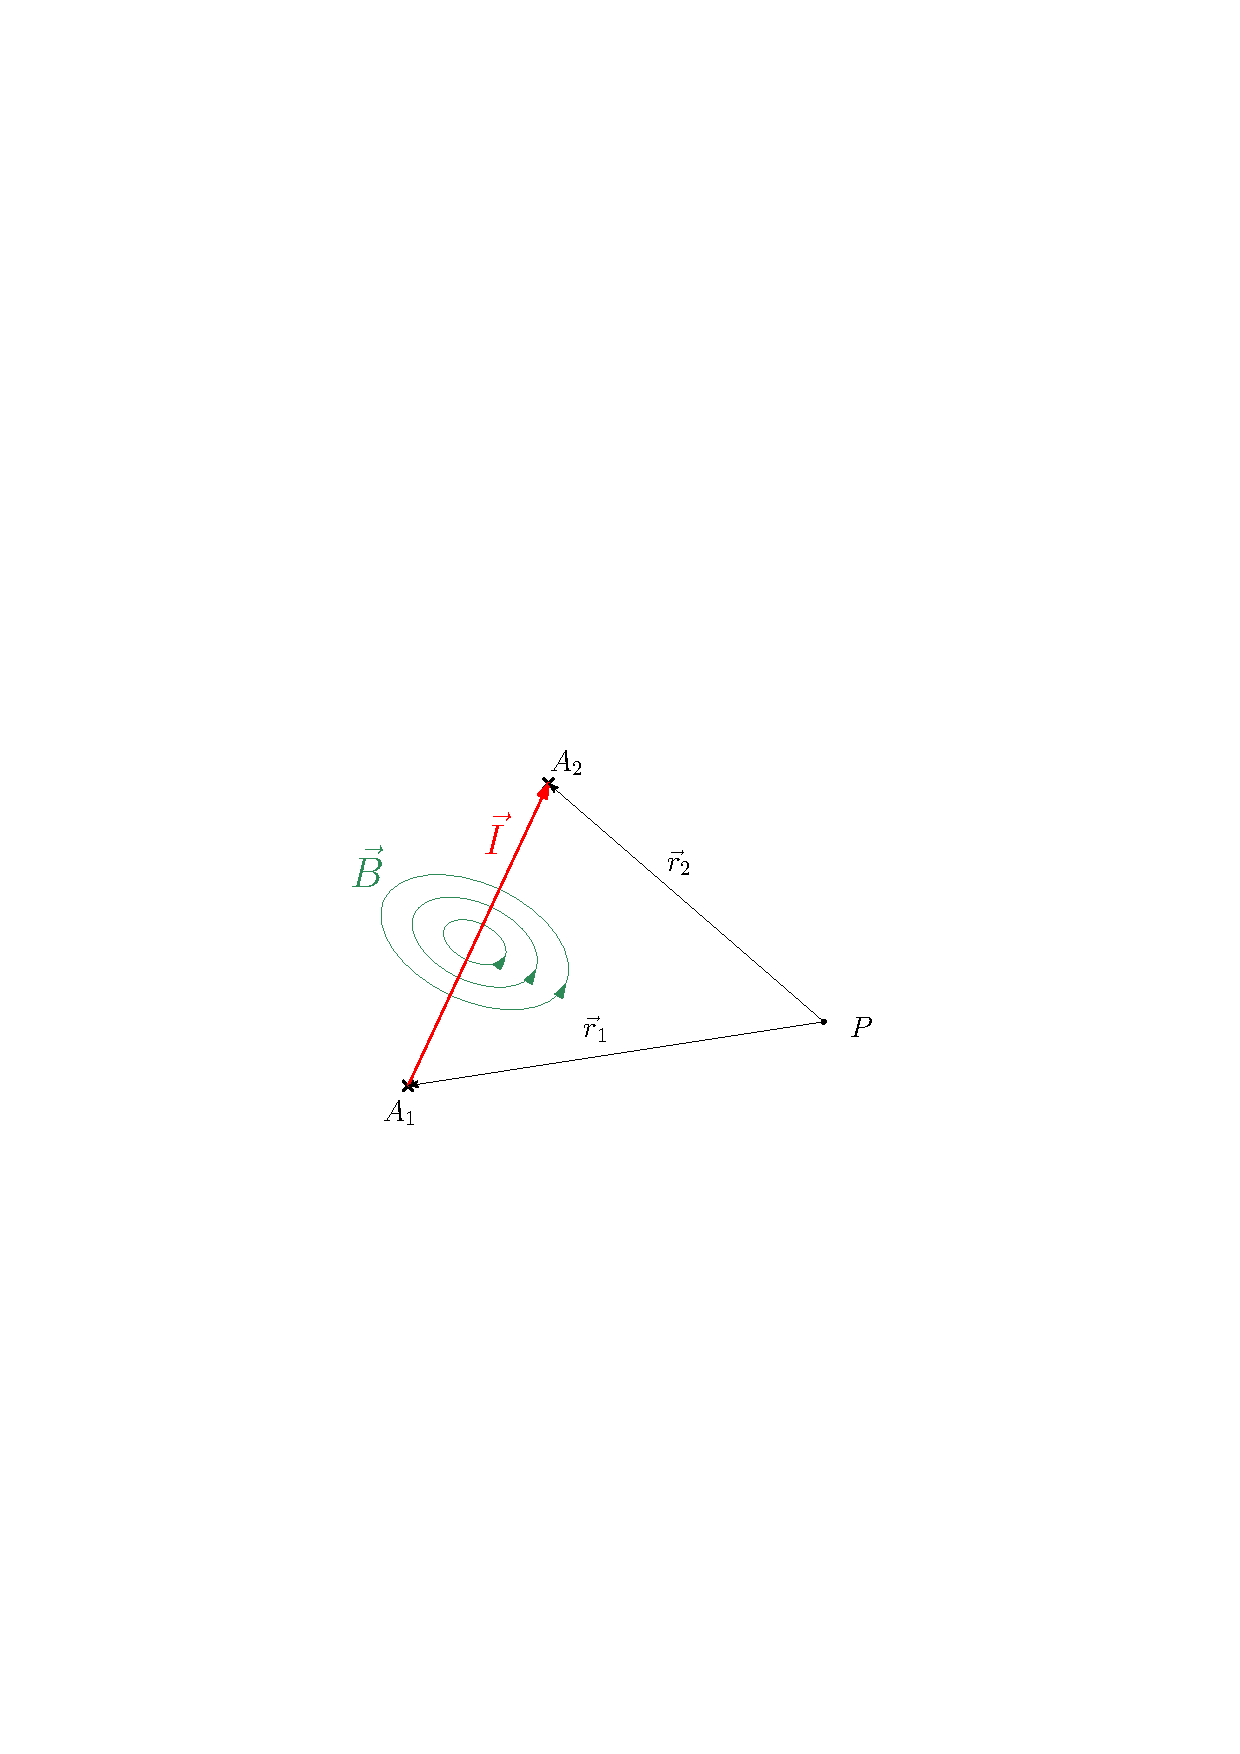
\includegraphics{images/KNAXSFigures/biot.pdf}}
      \caption{A line-current-segment is defined by a start point $A_1$, an endpoint $A_2$ and the magnitude of the current $\vec{I}$ that flows from $A_1$ to $A_2$.}
      \label{fig:definition line current segment}
    \end{figure}\\
    As we want to discretize our objects down to finite line-current segments, similar to the one shown in figure \ref{fig:definition line current segment}, we integrate along a line current segment and get:
    \begin{equation}
      \begin{aligned}
      \vec{B}_{i} &= \frac{\mu_0}{4\pi} \mathrm{d}\vec{L} \times \vec{I} \qquad \text{with} \\
      \mathrm{d}\vec{L} &= \left(\frac{\hat{r}_{1}+\hat{r}_{2}}{R+l}-\frac{\hat{r}_{1}+\hat{r}_{2}}{R-l}\right)\text{,} \\
      R&=|\vec{r}_{1}|+|\vec{r}_{2}| \text{,}\qquad l=|\vec{r}_{2}-\vec{r}_{1}|\qquad\text{and}\qquad \hat{r}_i = \frac{\vec{r}_i}{|\vec{r}_i|}\text{.}
      \end{aligned}
    \end{equation}
    Being able to use the superposition principle, it is possible to approximate complex shapes by numerous line-current-segments and simply sum up their individual field contributions $\vec{B}_{i}$ to get the overall resulting magnetic field:
    \begin{equation}
      \vec{B}_{total}=\sum_{i=1}^{N} \vec{B}_i
    \end{equation}
    Geometries composed of such line current segments can easily be tested by checking the validity of the Maxwell-equations. If, for example, the curl of the magnetic field $\vec{\nabla}\times\vec{B}_{total}$ is non-zero in vacuum, this is a hint that a current loop is not closed and that you should check your discretization.

    \subsubsection{Magnetic Dipole-Bars}
      The hall where the KATRIN experiment is housed consists mainly of concrete and ferro-magnetic steel. The steel rods inside the floor and the walls cause non-negligible, highly inhomogeneous magnetic stray-fields. As people have already foreseen that during the planning of the experiment, the KATRIN-hall was partially built with stainless steel that has a by far decreased magnetisation. However, there remains a strong magnetic component caused by the magnetic materials in the walls of the KATRIN-hall. \\
      Fortunately, it is known how the obstructed steel bars are magnetized: namely along their symmetry axis. In this case, one can make the simplifying approximation of a magnetic dipole with two magnetic charges $Q$ at both ends of the bar (see figure \ref{fig:definition magnetic dipole bar}).
      \begin{figure}[h]
	\centering \scalebox{0.9}{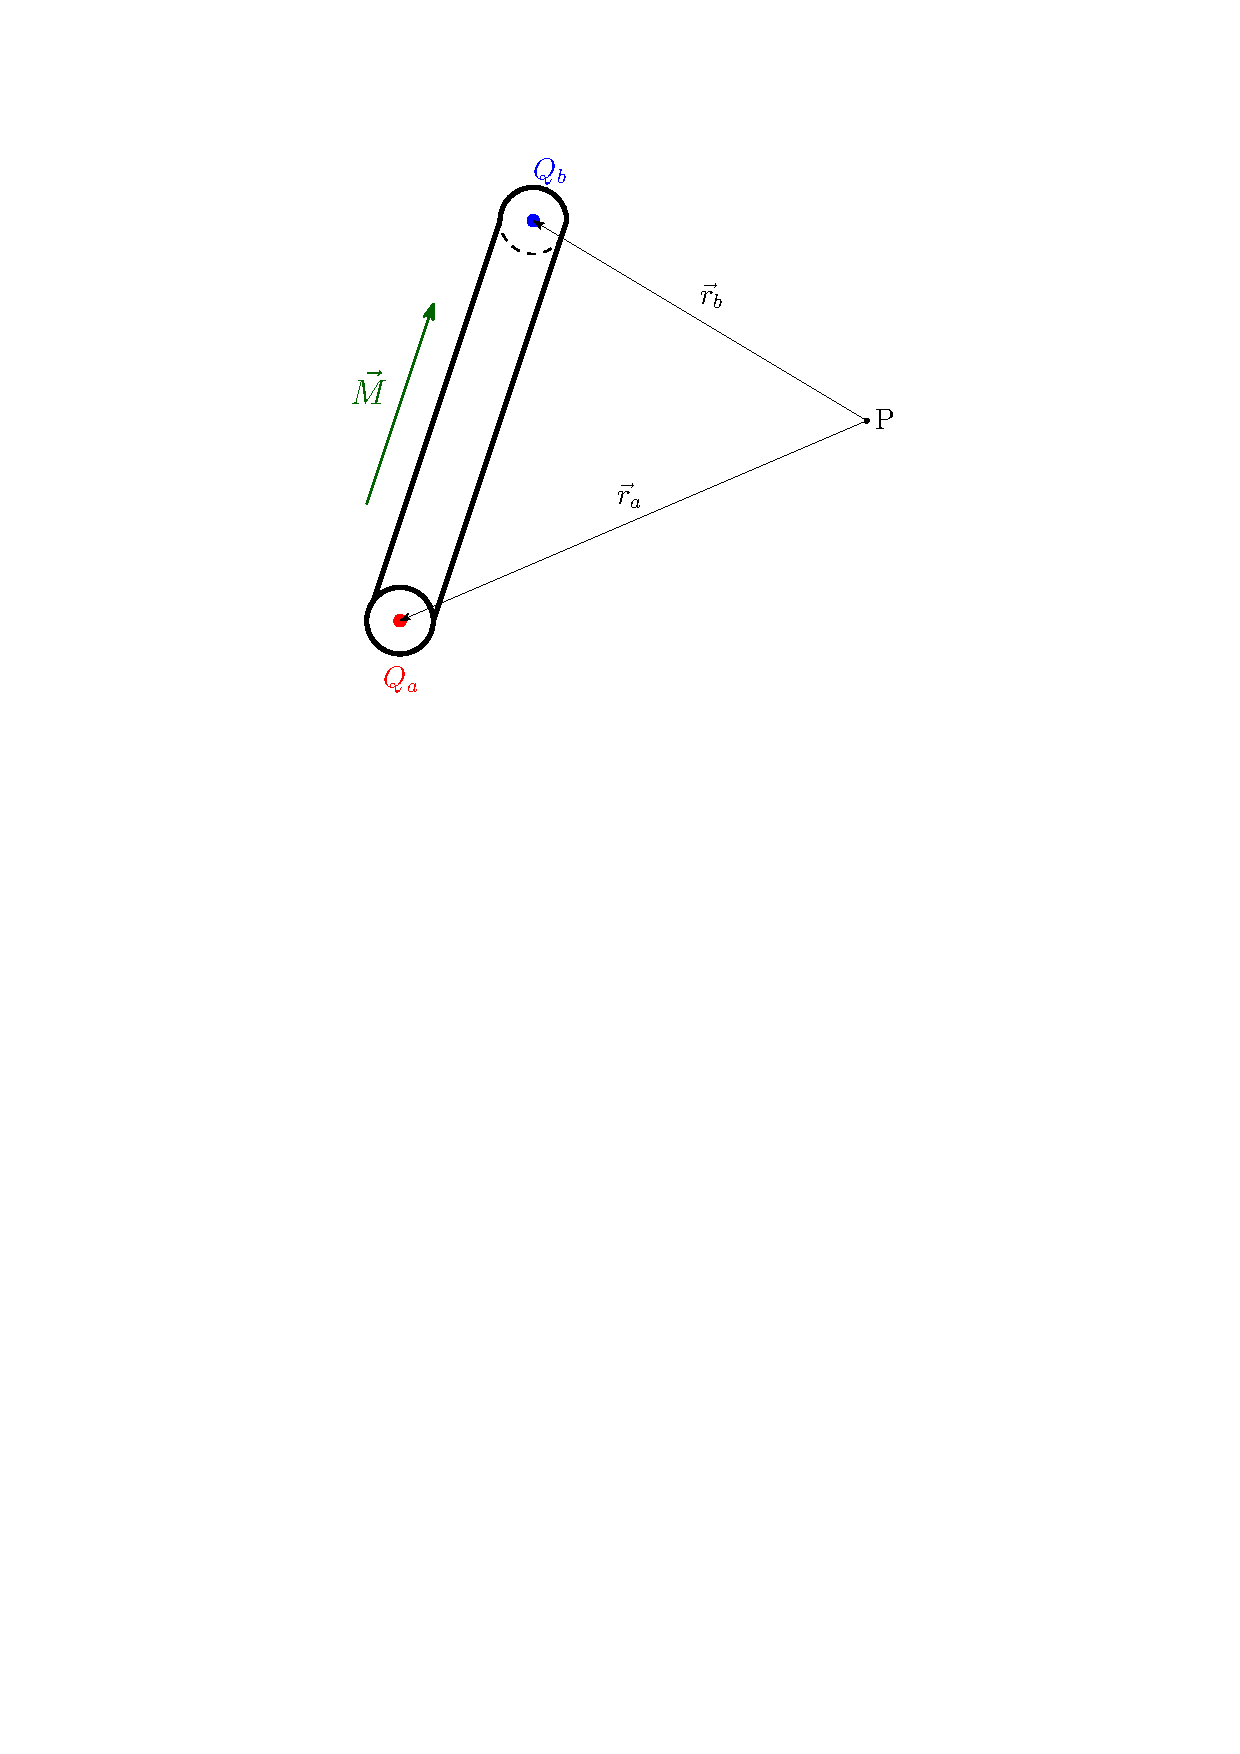
\includegraphics{images/KNAXSFigures/mag_bar.pdf}}
	\caption{The magnetic-dipole-bars are characterised by two magnetic charges at the ends of the bar, their distance and the radius of the bar.}
	\label{fig:definition magnetic dipole bar}
      \end{figure}\\
      The magnetic field of such a dipole can be easily calculated analogue to Coulomb's law:
      \begin{equation}
	\vec{B}_{i}(P) = -Q \frac{\mu_0}{4\pi}\left(\frac{\vec{r}_{a}}{|\vec{r}_{a}|^3}+\frac{\vec{r}_{b}}{|\vec{r}_{b}|^3}\right) \qquad \text{with} \qquad Q = |\vec{M}| \cdot\pi r^2
      \end{equation}
      $\vec{M}$ denotes the magnetisation and $r$ the radius of the dipole-bar. Again, to get the total magnetic field from all dipole-bars their contributions $B_{i}$ have to be summed up.
  \subsection{Three-Dimensional Hermite-Interpolation} % ZITAT M. EUPNER !!!!!!!!
    Interpolation methods are often employed when calculating the field of a static setup. The interpolation grid is plotted once in advance and every time the field needs to be evaluated in a certain point, it is interpolated and optionally scaled using the precomputed grid. The Hermite-interpolation, in contrast to the linear-interpolation does not only need the values at the grid points, but also their partial derivates. This results in a longer precomputation time, but as the accuracy of the Hermite-interpolation scales not just with the 2nd but with the 4th power of the grid distance, this is the preferred method to use when interpolating with relatively large grids. \\  
    Interpolating usually means a dramatic speed up of the field calculations, especially for non axisymmetric fields and still grants a high numeric precision.
  \subsubsection{Theory}
    \begin{figure}[h]
      \centering \scalebox{0.6}{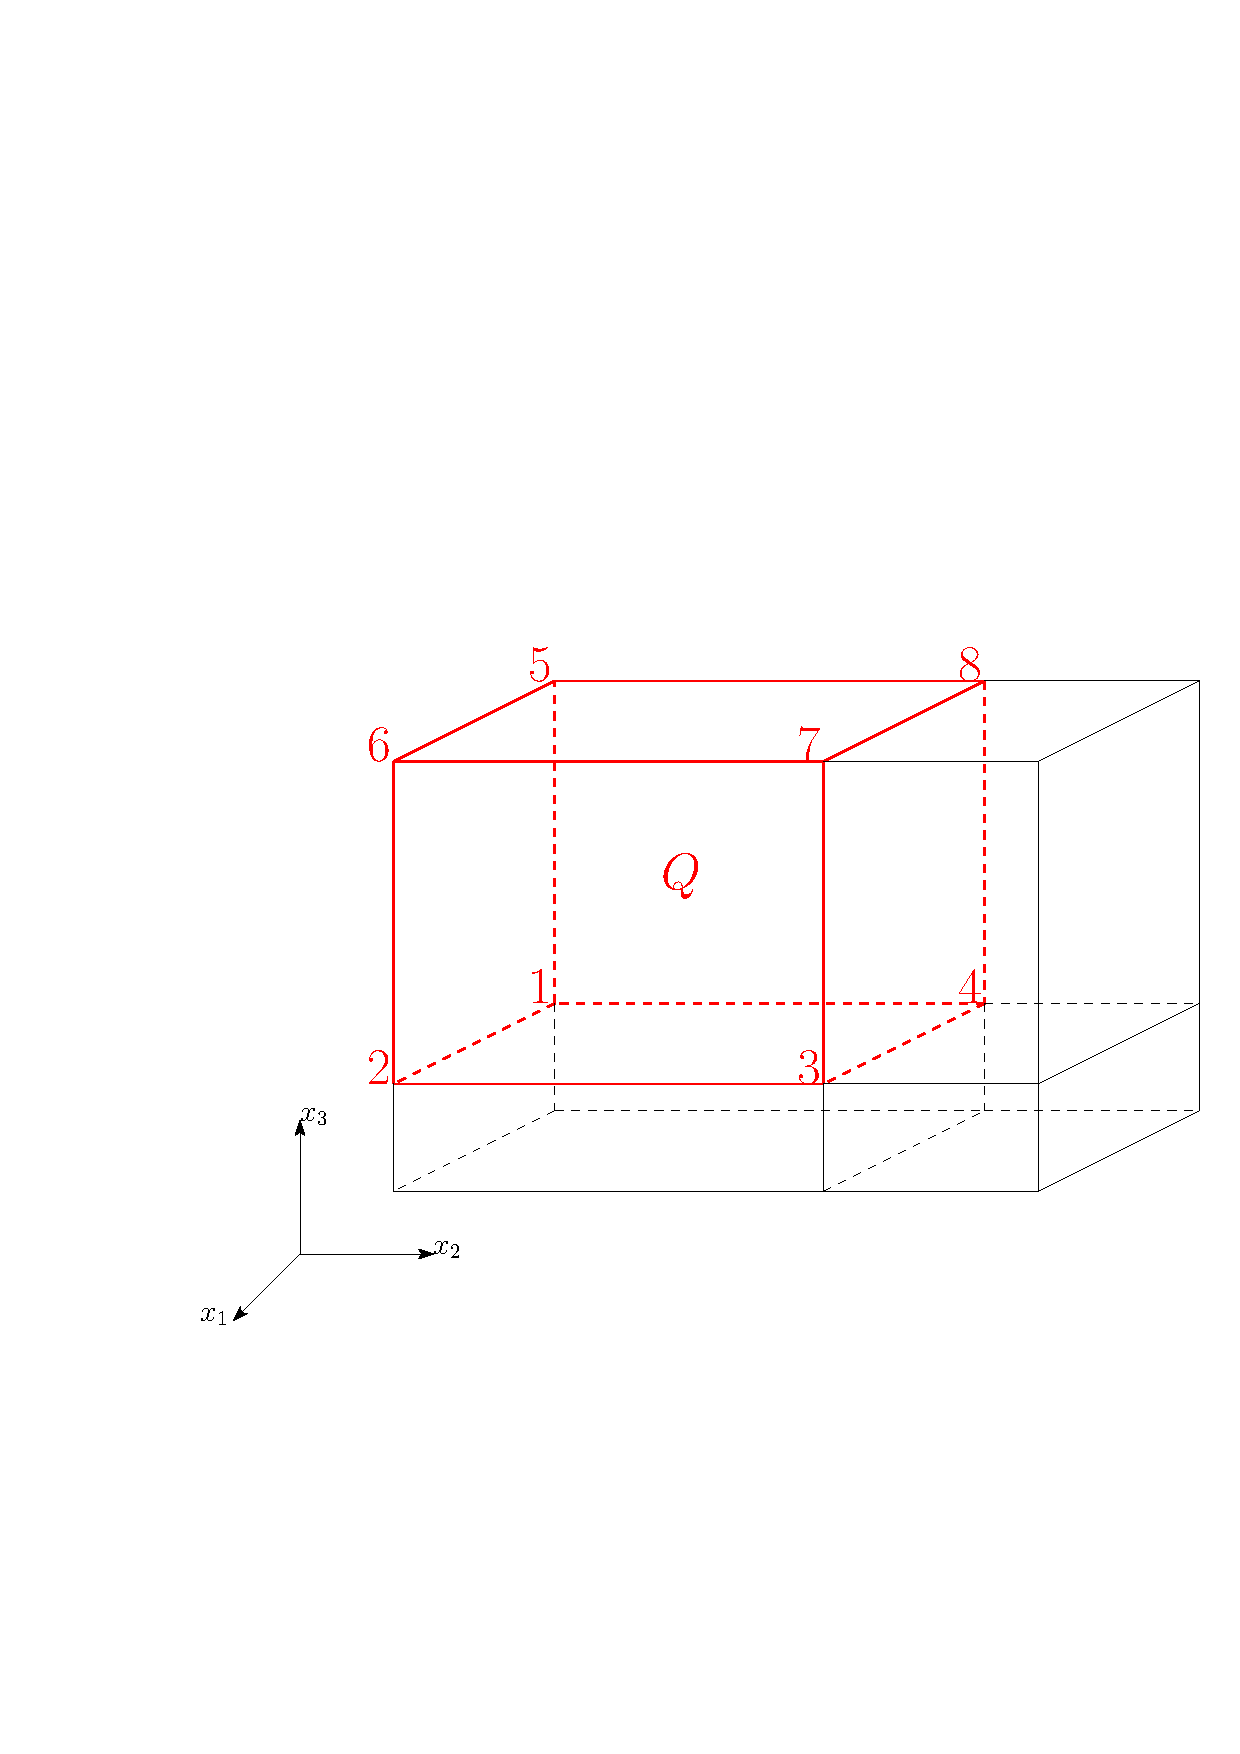
\includegraphics{images/KNAXSFigures/cuboid.pdf}}
      \caption{Example grid consisting of cuboids.}
      \label{fig:grid of cuboids}
    \end{figure}
    We are given a rectangular, three-dimensional grid that consists of cuboids (see fig. \ref{fig:grid of cuboids}. A cuboid Q of this grid can be described as follows.
    \begin{equation}
	    Q := \left\lbrace \left( x_{1},x_{2},x_{3} \right) ~ \epsilon ~  \mathbb{R}^{3} \;  / \;  x_{ui} < x_{i} < x_{oi} \;  ; \;  i=1,2,3  \right\rbrace 
    \end{equation}
    Through a coordinate-transformation of the form:
    \begin{equation}
	    \begin{aligned}
		    u_{i} &= \frac{x_{i}-x_{mi}}{a_{i}} \quad  \text{with} \\
		    x_{mi} &= \frac{x_{oi}+x_{ui}}{2} \quad  \text{and} \quad  a_{i} = \frac{x_{oi}-x_{ui}}{2}
	    \end{aligned}
    \end{equation}
    we project $Q$ to the unit-cube $E$:
    \begin{equation}
	    E := \left\lbrace \left( u_{1},u_{2},u_{3} \right) ~ \epsilon ~  \mathbb{R}^{3} \;  / \;  -1 < u_{i} < 1 \;  ; \;  i=1,2,3  \right\rbrace
    \end{equation}
    Now we define a function $g(\vec{u})$ on $E$ with:
    \begin{equation}
	    f(\vec{x}) = g(\vec{u}(\vec{x}))
    \end{equation}
    The goal is to interpolate $g(\vec{u})$ within the unit-cube $E$. Therefore, we need to know the function-values at the eight corner points $\vec{u}_{i}$ as well as their first partial derivatives. We combine them into a Matrix $\mathcal{G}$, where the function-values fill one column:
    \begin{equation}
	    \mathcal{G}_{i0} := g(\vec{u}_{i}) ~ (i=1,...,8)
    \end{equation}
    and the others are filled by their partial derivatives:
    \begin{equation}
	    \mathcal{G}_{ij} := \left\lbrace \frac{\partial g(\vec{u})}{\partial u_{j}} \right\rbrace_{\vec{u}=\vec{u}_{i}} \quad (i=1,...,8 \; ; \; j=1,2,3)
    \end{equation}
    The next step is to define a so called Interpolation-polynomial:
    \begin{equation}
	    G(\vec{u})= \sum_{i=1}^{8} \sum_{j=0}^{3} \mathcal{G}_{ij} \phi_{ij}(\vec{u})
    \end{equation}
    The coefficient-polynomials $\phi_{ij}$ are chosen, so that $G(\vec{u}_{k})=\mathcal{G}_{k0}$ and \\$\left\lbrace \frac{\partial g(\vec{u})}{\partial u_{1}} \right\rbrace_{\vec{u}=\vec{u}_{k}} = \mathcal{G}_{k1}$. This leads to the following constraints:
    \begin{equation}
    \phi_{ij}(\vec{u}_{k})=\delta_{ik}\delta_{j0} \qquad \mbox{and} \qquad \left\lbrace \frac{\partial \phi_{ij}(\vec{u})}{\partial u_{1}} \right\rbrace_{\vec{u}=\vec{u}_{k}} =\delta_{ik}\delta_{j1}
    \end{equation}
    These are fulfilled, if we define $\phi_{ij}$ like:
    \begin{equation}
	    \phi_{ij}(\vec{u}) := u_{ij} \prod_{k=1}^{3} \varphi_{jk} (u_{ik} \cdot \vec{u}_{k})
    \end{equation}
    where $\varphi_{jk}$ is given by:
    \begin{equation}
	    \varphi_{jk}(t) := \frac{1}{4} \left[ \left( 2+3t-t^{3}\right) + \left( -3-4t+t^{2}+2t^{3}\right) \delta_{jk} \right] \quad \mbox{and} \quad u_{i0}:=1
    \end{equation}
    \\
    In order to interpolate the function $f(\vec{x})$ within the cuboid $Q$, we have to follow some simple steps:
    \begin{enumerate}
	    \item calculate the function-values and their partial derivatives of $f$ regarding $\vec{x}$ at all 8 corner points,
	    \item transform them into the unit-cube $E$:
		    \begin{equation}
		    \mathcal{G}_{ij} =
		    \begin{cases}
			    a_{j} \cdot \left\lbrace \frac{\partial f(\vec{x})}{\partial x_{j}} \right\rbrace_{\vec{x}=\vec{x}_{i}} & \text{if} \quad j>0 \\
			    f(\vec{x}_{i}) & \text{if} \quad j=0
		    \end{cases}
		    \end{equation}
	    \item and interpolate function-values and derivatives at any point $\vec{x} ~ \epsilon ~ Q$ :
		    \begin{equation}
		    \begin{aligned}
			    \frac{\partial f(\vec{x})}{\partial x_{j}} &= a_{j}^{-1} \cdot \frac{\partial G(\vec{u}(\vec{x}))}{\partial u_{j}} \qquad j=1,2,3 \\
			    f(\vec{x}) &= G(\vec{u}(\vec{x}))
		    \end{aligned}
		    \end{equation}
    \end{enumerate}
    Interpolation methods  yield the possibility of a scalable precision. When a high precision is needed, the distance between the grid points can be chosen very small and in the contrary case, when a lower precision is sufficient, it can be chosen rather large. This has no impact on the actual computation time, just on the time needed to compute the initial grid.
    \subsection{Implementation}
      All KNAXS-classes derive from the \texttt{Field} base-class and \texttt{Magfield} respectively. The integrated Biot-Savart method is implemented in a class called \texttt{BiotSavart} and the field calculation of the magnetic dipole-bars in a class called \texttt{MagMaterials}. They are both organized in a very similair way: They both have a member-container that holds their particular segments:
      \begin{itemize}
	\item \texttt{Line(Double\_t current, TVector3 startPosition, TVector3 endPosition)} represents a line-current segment that is defined through to points and a current running from one point to the other. It has methods to set and get the start- and endpoint of the line and the current it is carrying. \texttt{FieldInLine(TVector3 p)} returns the magnetic field ($\vec{B}$) caused by the segment at the position \texttt{p}.
	\item \texttt{Bar(TVector3 P1, TVector3 P2, Double\_t magnetization, Double\_t radius, Double\_t susceptibility)} represents a magnetized bar and is defined through two points at the end, a magnetization pointing from one point to the other, a radius and the magnetic susceptibility of the material. It has methods to get and set these quantities. \texttt{GetHField(TVector3 p)} returns the magnetic field ($\vec{H}$) caused by the segment at the position \texttt{p}.
      \end{itemize}
      These elements can be added to the field-objects through the \texttt{AddLine(Line)}/\texttt{AddBar(Bar)} methods. The total magnetic field at a given position can be retrieved through the \texttt{GetField(TVector3)} method. In this method, the contributions of the single elements are simply summed up and the total field is then returned.
      \\
      The interpolation classes are a bit more complicated. The base method was implemented into the class \texttt{FieldInterpolation}. The classes \texttt{MagfieldInterpolate} and \texttt{ElfieldInterpolate} inherit from this class, and of course from the abstract field base classes. Figure \ref{fig:Magfieldinterpolate overview} shows a principle diagram of the \texttt{MagfieldInterpolate} class and figure \ref{fig:Elfieldinterpolate overview} of the \texttt{ElfieldInterpolate} class, respectively.
      \begin{figure}[h]
		\centering 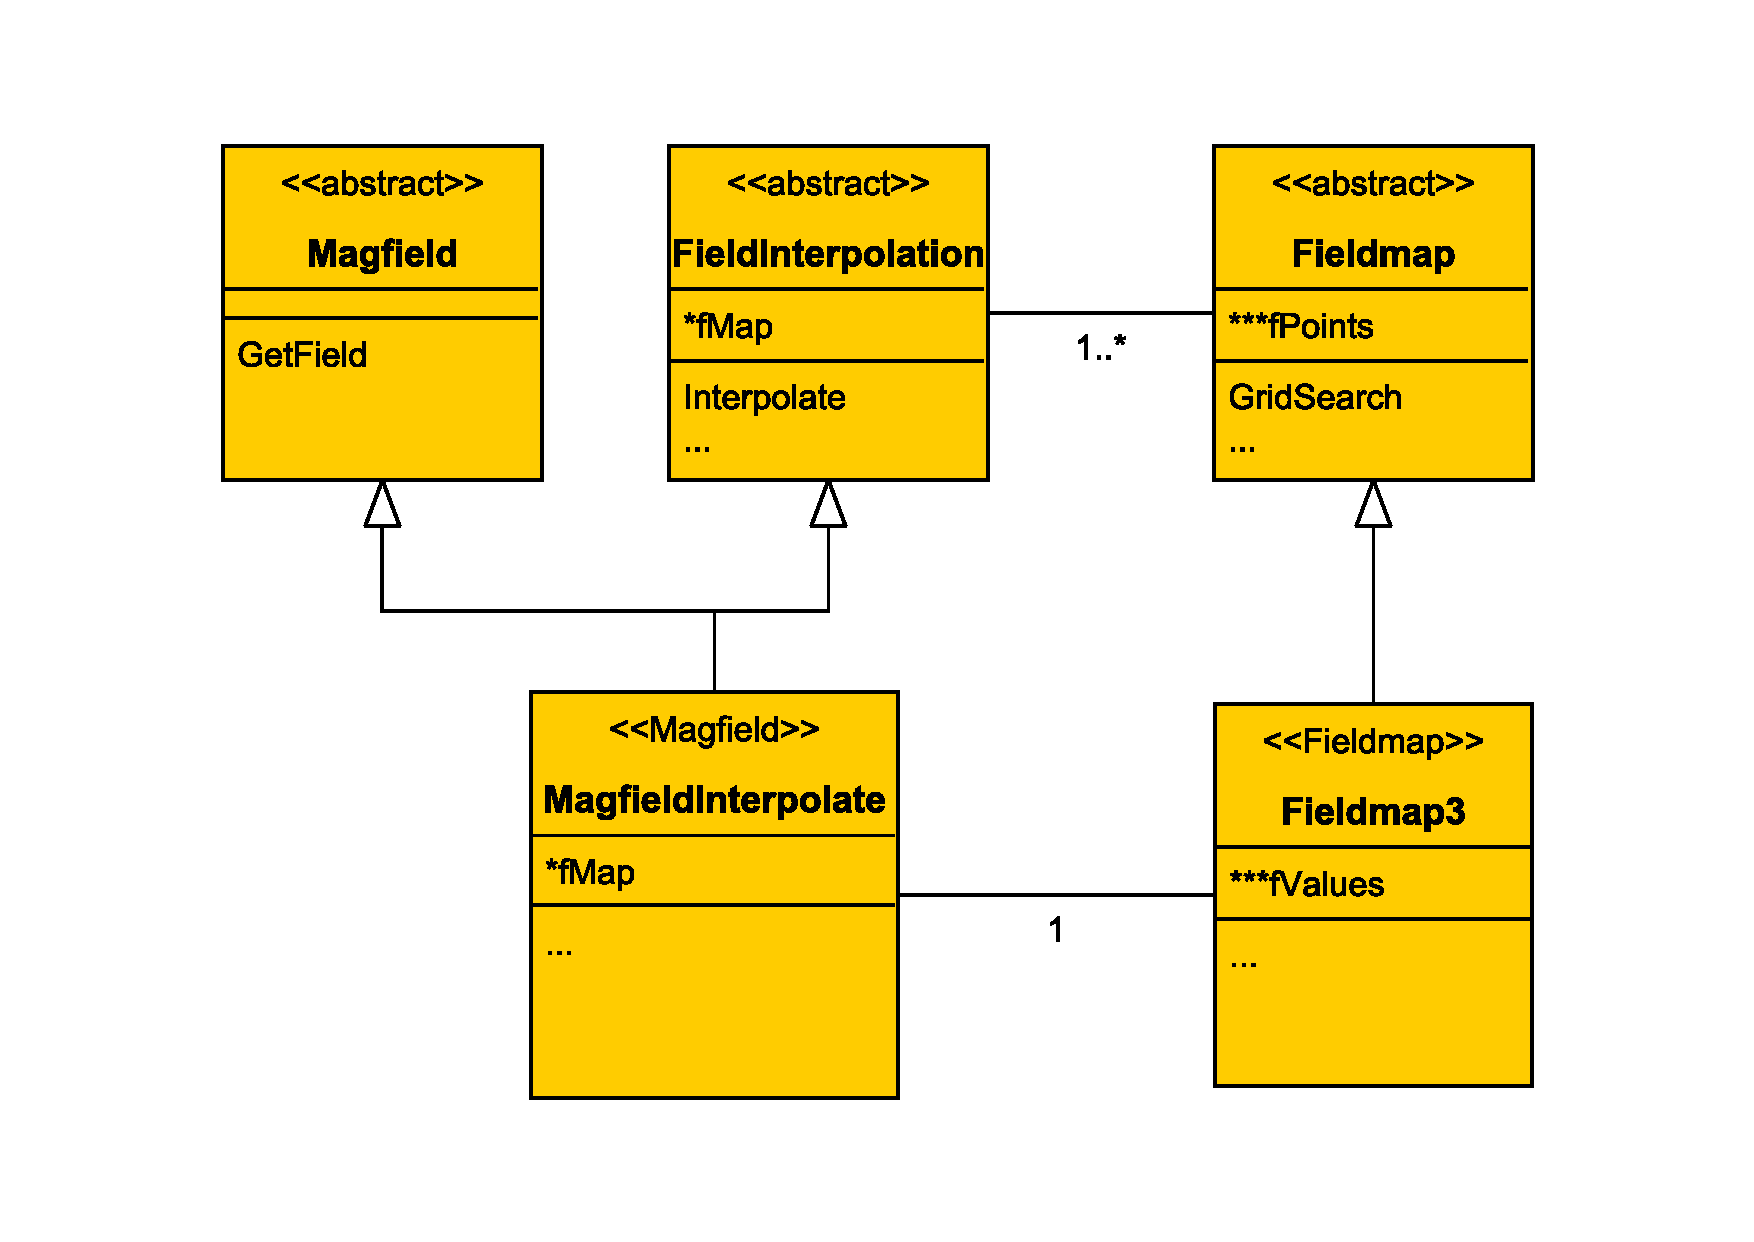
\includegraphics[width=0.9\textwidth]{images/KNAXSFigures/mag_interpolation_uml.pdf}
		\caption{Overview of the \texttt{MagfieldInterpolate} class: It inherits from the abstract classes \texttt{Magfield} and \texttt{FieldInterpolation}. It has one member object of the class \texttt{Fieldmap3} that inherits from the abstract class \texttt{Fieldmap}.}
		\label{fig:Magfieldinterpolate overview}
      \end{figure}
      Objects of the stereotype \texttt{FieldInterpolation} store one or more interpolation grids in objects of the stereotype \texttt{Fieldmap}. These grids contain for example the scalar electric potential with just one value at a grid point in case of a \texttt{Fieldmap1} object, and the grids for the three-dimensional vector fields, that have three values and nine partial derivatives in one grid point, are stored in  \texttt{Fieldmap3} objects. In case of rotational symmetry, one can also use the \texttt{Fieldmap2} objects, but this has to be specified explicitly by the user.
      \begin{figure}[h]
		\centering 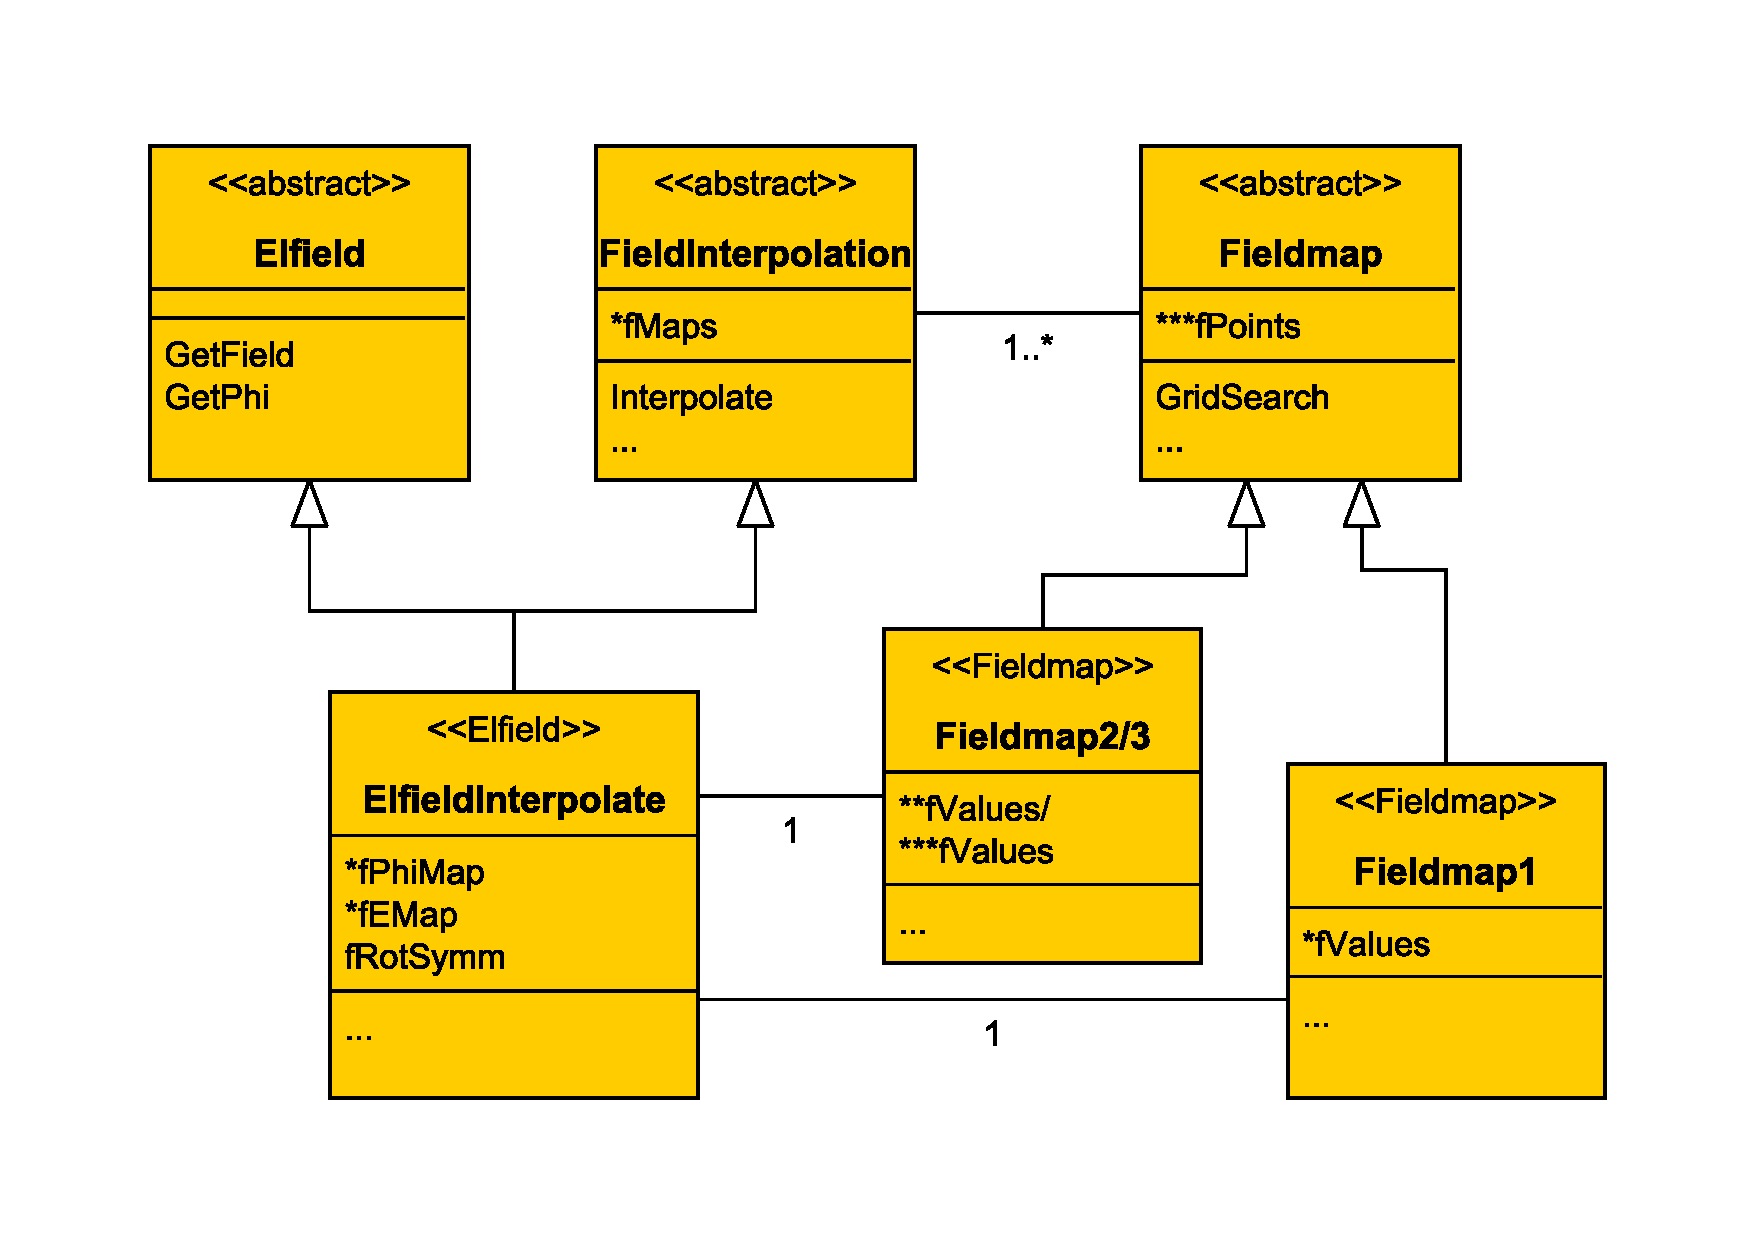
\includegraphics[width=0.9\textwidth]{images/KNAXSFigures/el_interpolation_uml.pdf}
		\caption{Overview of the \texttt{ElfieldInterpolate} class: It inherits from the abstract classes \texttt{Elfield} and \texttt{FieldInterpolation}. It has two member objects that inherit from the abstract class \texttt{Fieldmap}: a \texttt{Fieldmap1} object, in which the interpolation grid for the electric potential is stored and a \texttt{Fieldmap2} or \texttt{Fieldmap3} object, depending if the field is axially symmetric, in which the interpolation grid for the electric field is stored.}
		\label{fig:Elfieldinterpolate overview}
      \end{figure}
      In order to pre-compute a grid, the virtual methods \texttt{CreateMagFieldmap} and \texttt{CreateElFieldmap} that are members of the \texttt{Fieldmap} classes have to be called. They compute a grid of the specified \texttt{Magfield} or \texttt{Elfield} object, respectively. \texttt{CreateElfieldmap} actually creates two field maps, one for the electric field and one for the potential. Afterwards they are saved to a file and can be read in with the virtual method \texttt{ReadMapFromFile}.
% KEMField documentation for the Kassiopeia Guide

\section{Comprehensive Field Simulation: KEMField}\label{sec:KEMField}

\subsection{Electrostatic Solver: The RobinHood Method}

The Robin Hood method was developed by Predrag Lazic,  Hrvoje Stefancic, and Hrvoje Abraham~\cite{RH1,RH2} and the reader is encouraged to read the cited literature.  At its core, Robin Hood is a matrix inversion algorithm but, as such, it is particularly suited for electrostatic problems, especially those whose boundary conditions are well-defined. Let us first define the problem to be solved, and then discuss the implementation of Robin Hood toward its solution.

Consider the case where one wishes to know the potential, $U(\vec{x})$ at some point in space ($\vec{x}$).  To find the potential, one needs to calculate the contribution from each charge sub-element (with charge density $\sigma_i$) which contributes to the potential.  

\begin{equation}
U(\vec{x}) = \int_{\partial V} G(\vec{x},\vec{x'}) \sigma(\vec{x}') dS'
\end{equation}

\noindent Here, the integration is carried over some surface $dS'$ with a charge density $\sigma$ at a location $\vec{x}'$.  Green's function, $G(\vec{x},\vec{x'})$ is given by the expression

\begin{equation}
G(\vec{x},\vec{x'}) =  \frac{1}{4 \pi \epsilon_0} \frac{1}{|\vec{x}-\vec{x}'|}
\end{equation}

With discretization, one imposes the assumption that the surface charge density is constant across $dS'$.  The integration therefore reduces to a sum

\begin{equation}
U_i = \sum_{j=1}^N I_{ij} \sigma_j
\label{eq:potential}
\end{equation}

\noindent where $U_i$ is the potential of the sub-element $i$, $\sigma_j$ is the charge density of sub-element $j$ of $N$ and $I_{ij}$ is given by...

\begin{equation}
I_{ij} = \frac{1}{4\pi\epsilon_0}\int_{\Delta S_j} \frac{dS_j}{|\vec{r}_i - \vec{r}_j|} 
\end{equation}

In the case where one is dealing with only metal conductors, all such charges reside at the surfaces.  Furthermore, all metal surfaces are at {\em equipotential} (either defined by the configuration of the experiment or by the electrostatic configuration itself).  This essentially sets up the necessary boundary conditions one needs to solve.  The charge densities $\sigma_i$ will arrange themselves until all the surfaces in the problem are indeed at equipotential.  Once the charge configuration is known, then the potential everywhere in space (not just at the surfaces) can be known as well\footnote{This last condition is guaranteed by the nature of Laplace's equation.}.  

Boundary element methods are directed at solving the above matrix, and the Robin Hood method is no exception.  At its heart, it is a variation of the boundary element method.  However, it appears to be {\em the most efficient} implementation of BEM, both in terms of computation time and memory use.  

\subsubsection{Implementation with Conductors in Isolation}

To describe the algorithm, consider the following simple example.  An isolated metal cube has a total charge $Q$ distributed over its surface.  We subdivide the surface into smaller sub-elements (typically rectangles and/or triangles, though this is not necessary), each with a small amount of charge $q$ over each of their surfaces.  The initial assignment of charges can be random since we do not know the proper configuration at this stage.  Using this (incorrect) charge configuration, we can therefore compute the potential at each sub-element using Eq.~\ref{eq:potential}.  Of course, the potential across the surface at this point will {\em not} be an equipotential because the charge configuration is incorrect.

To correct the charge configuration, we select two sub-elements from the configuration ($m$ and $n$).  The sub-elements are selected such that they are furtherest away from the average potential.  We then {\em redistribute} the charges such that they are both at the same potential.  For the case of two sub-elements, there is an exact solution to the amount of charge that needs to be moved from one element to the other.

\begin{equation}
\delta \sigma = \frac{U_m - U_n}{I_{mm} + I_{nn} - I_{mn} - I_{nm}}
\end{equation}

\noindent where $U_{m,n}$ is the potential at the two selected points. The new potential due to this redistribution is given by

\begin{eqnarray}
U_m' = U_m - I_{mm}\delta \sigma + I_{mn}\delta \sigma\\
U_n' = U_n + I_{nn}\delta \sigma - I_{nm}\delta \sigma
\end{eqnarray}

The charge exchange of $\delta \sigma$ has two effects. First, it now forces $U_m'$ and $U_n'$ to be at the same potential and secondly, these new charges propagate their effects to their neighboring elements.  This allows the solution to quickly converge.  The process is then repeated until the maximum difference between the equipotential solution and $U_i$ falls below some pre-determined user-defined threshold.

\subsubsection{Implementation with Conductors at a Defined Potential}

As another example, let us consider now the case where the cube is held at a fixed potential $U_0$.  The algorithm is very similar to the case of the isolated cube, except one can relax the charge conservation condition (because effectively one can extract the charge from an external source).  Again, one initially randomizes the charge distribution and then selects two elements whose potential is furthest away from the equipotential $U_0$.  The amount of charge added to the two selected elements ($k$ and $l$) is given by the following expression:

\begin{eqnarray}
\delta \sigma_k = \frac{(U_0 - U_k)I_{ll} - (U_0-U_l)I_{kl}}{I_{kk} I_{ll} -I_{kl}I_{lk}}\\
\delta \sigma_l = \frac{(U_0 - U_l)I_{kk} - (U_0-U_k)I_{kl}}{I_{kk} I_{ll} -I_{kl}I_{lk}}
\end{eqnarray}

The adjusted potential is given by 

\begin{eqnarray}
\label{eq:charge_exchange}
U_k' = U_k + I_{kk} \delta \sigma_k + I_{kl} \delta \sigma_l \\
U_l' = U_l + I_{ll} \delta \sigma_l + I_{kl} \delta \sigma_k
\end{eqnarray}

The solution quickly converges, as the added charges equalize not just the selected elements, but its nearest neighbors as well.

\subsubsection{Charge Exchange Generalization}

For both the insulated and non-insulated conductors, we have shown the solution for the case when two electrodes exchange/add/subtract charges.  We can generalize the solution to the case of M electrodes exchanging charge, where $1 \le M \le N$.  For the case of electrodes held at fixed potential, this is equivalent to the inversion of a $M \times M$ matrix:

\begin{equation}
\sum_{j = 1}^{M} I_{ij} \sigma_j = U_i
\end{equation}

\noindent where $I_{ij}$ is the $M \times M$ Coulomb matrix as defined previously.  Both indexes $i$ and $j$ range from 1 to $M$. Note that for M=2, one reproduces Eq.~\ref{eq:charge_exchange}.

The same generalization can be made for the insulated charge case.  Here, one must explicitly introduce the conservation of charge as part of the matrix to be solved.   In general, one can impose the conservation of charge as follows:

\begin{equation}
\sum_{j=1}^{M} \sigma_j = 0
\end{equation}

As for the condition imposed by the equipotential surface, one realizes that all the potentials at each altered electrode are identical.  One way to write this condition is as follows:

\begin{equation}
\sum_{j=1}^{M}(I_{i,j} - I_{i+1,j}) \sigma_j = U_{i+1}-U_i
\end{equation}

Note that index $i$ ranges only from 1 to $M-1$.  The combination of the two constraints produces an $M \times M$ matrix equation which can be inverted to solve for $\sigma_j$.  Note that for the isolated conductor, $M > 1$.

\subsubsection{Advantages and Caviats}

The Robin Hood method is very effective in computing the charge configuration within the context of computing algorithms for a number of reasons, some of which are iterated below:

\begin{itemize}
\item The algorithm searches for the maximum deviation from equipotential for each sub-element.  As such, it can readily make use of functions such as MAX/MIN, which are extremely efficient for arrays.  Furthermore, since it corrects elements which are furthest away from the solution (and those elements affect those around them, due to the properties of Green's function), there is rapid convergence of all charges.
\item In implementing the charge correction, it is most advantageous to recompute the elements $I_{ij}$.  In doing so, there is no need to create a large array.  As such, the memory allocation grows as $N$ rather than $N^2$.  Direct matrix inversion techniques require either $N^2$ or, in the most effective implementation of these systems, $N \log{(N)}$.
\item Since the algorithm is step-oriented, it can be very effectively be distributed to multiple processors.  Therefore, implementation on parallel systems (such as MPI) is straightforward.
\end{itemize}

In the next section, we will discuss the speed and accuracy of this algorithm.  In order to ensure convergence, the user needs to keep in mind that the matrix must possess the following properties:

\begin{itemize}
\item  {\it Diagonal Dominant:}  The algorithm converges only if the matrix being solved is diagonally dominant.  This condition is guaranteed due to the nature of Green's function for electro- and magneto- statics~\cite{Gluck}.
\item  {\it Linearity:}  This condition is guaranteed due to the nature of Maxwell's equation.
\item  {\it Uniqueness:}  If two or more elements are defined but their centers overlap, the solution is infinite and the solution quickly diverges.  In fact, RH by virtue of this property can quickly discover if elements overlap.  Note that this latter condition is a problem with BEM methods as well.
\end{itemize}

\subsubsection{Verification}

The Robin Hood algorithm has been successful implemented in KATRIN's Kassiopeia Monte Carlo framework, within the context of KEMField.  Its implementation is similar to BEM in that the electrode properties need to be defined prior to solving for the charge distribution.  The algorithm has been adapted for both single and parallel processing (MPI), though the majority of the tests described have been executed on a single processor (Mac OS X 10.6.4, 2.53 GHz Intel Core 2 Duo processor).  Since RH is most effective as a 3D discrete solver, we typically discretize the surfaces of our test electrodes into rectangles and triangles, though any electrode surface geometry can be used.  RH can be implemented to stop when a certain accuracy is reached or a certain number of iterations are processed.  The accuracy is computed using the formula

\begin{equation}
\epsilon = \frac{\sqrt{\frac{1}{N}\sum_i^N (U_i - U_0)^2}}{U_0}
\end{equation}

\noindent where $U_i$ is the potential at electrode $i$ and $U_0$ is the fixed potential at surface.  For these initial tests, we stop the iteration whenever $\epsilon < 10^{-15}$ or the number of iterations exceeds 200,000.

\subsection{Unit Cube}

Our first test has been conducted on a unit cube.  The capacitance of a unit cube in normalized units ($1/4\pi\epsilon_0$) is $0.66067786 \pm 8 \times 10^{-8}$\cite{RH2}\footnote{Incidentally, the most accurate calculation of the cube capacitance was achieved using the RH method (see citation).}.  The cube is discretized in a number of triangles and electrodes and the charge is then computed assuming the potential is held fixed at 1 V.  Table~\ref{tab:cube} shows the results using RH.

\begin{figure}[htbp]
\begin{center}
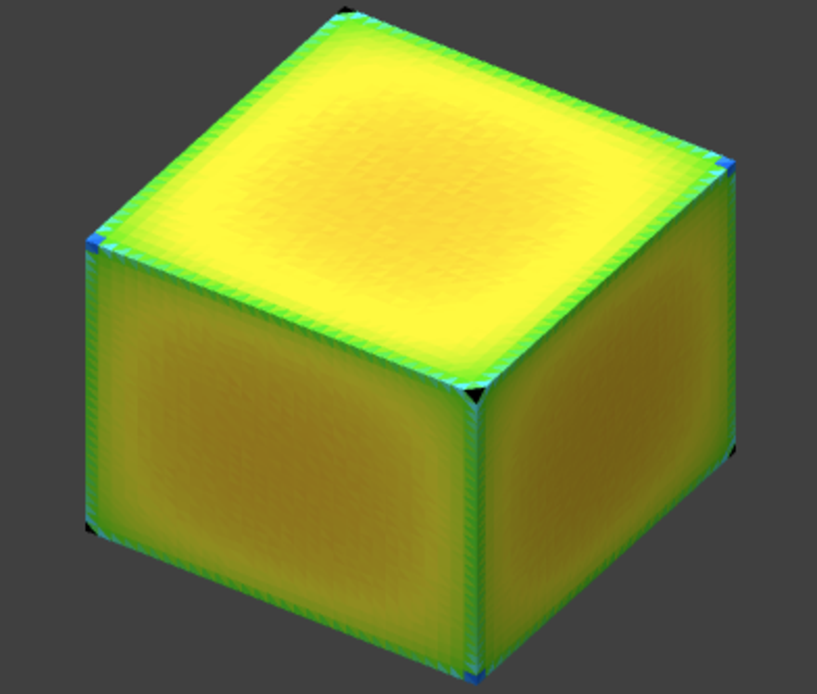
\includegraphics[width=0.6\textwidth]{images/KEMFieldPlots/cube_pic.pdf}
\caption{Charge distribution on discrete cube held at fixed potential.}
\label{fig:thecube}
\end{center}
\end{figure}

\begin{table}[htdp]
\caption{Unit capacitance of a cube as calculated by Robin Hood using $N$ electrodes.  Accuracy reports on the percentage difference to a previously calculated cube capacitance.  All sub-elements are the same size (no refinement near edges), except where indicated.}
\begin{center}
\begin{tabular}{|c|c|c|c|c|}
\hline
Test No. & Number of Elements & Accuracy & Scaling & Number of Iterations \\
\hline
1 & 660 & 0.23\% & fixed & 8000 \\ 
2 & 2520 & 0.13\% & fixed & 30,000 \\
3 & 10,800 & 0.08\% & fixed & 50,000 \\
4 & 15,300 & 0.04\% & fixed & 190,000 \\
5 & 60,600 & 0.01\% & fixed & 200,000 \\
6 & 19,200 & 0.0046\% & variable & 30,000 \\
\hline
\end{tabular}
\end{center}
\label{tab:cube}
\end{table}%

For test cases 1 and 2, we also computed the capacitance using a more standard Boundary Element Method.  In each case, the results were identical.  Running test cases 3-6 on a single processor using BEM is extremely time consuming and was therefore abandoned.  In general, changing the length scale as one approaches the edge of the cube increases the convergence and accuracy of the results (for example, case 6 took 20 minutes to converge with an accuracy on the capacitance of better than $5\times10^{-5}$). Similar tests were conducted making use of MPI.  Results of these tests are shown in Figure~\ref{fig:cube_results}.

\begin{figure}[htbp]
\begin{center}
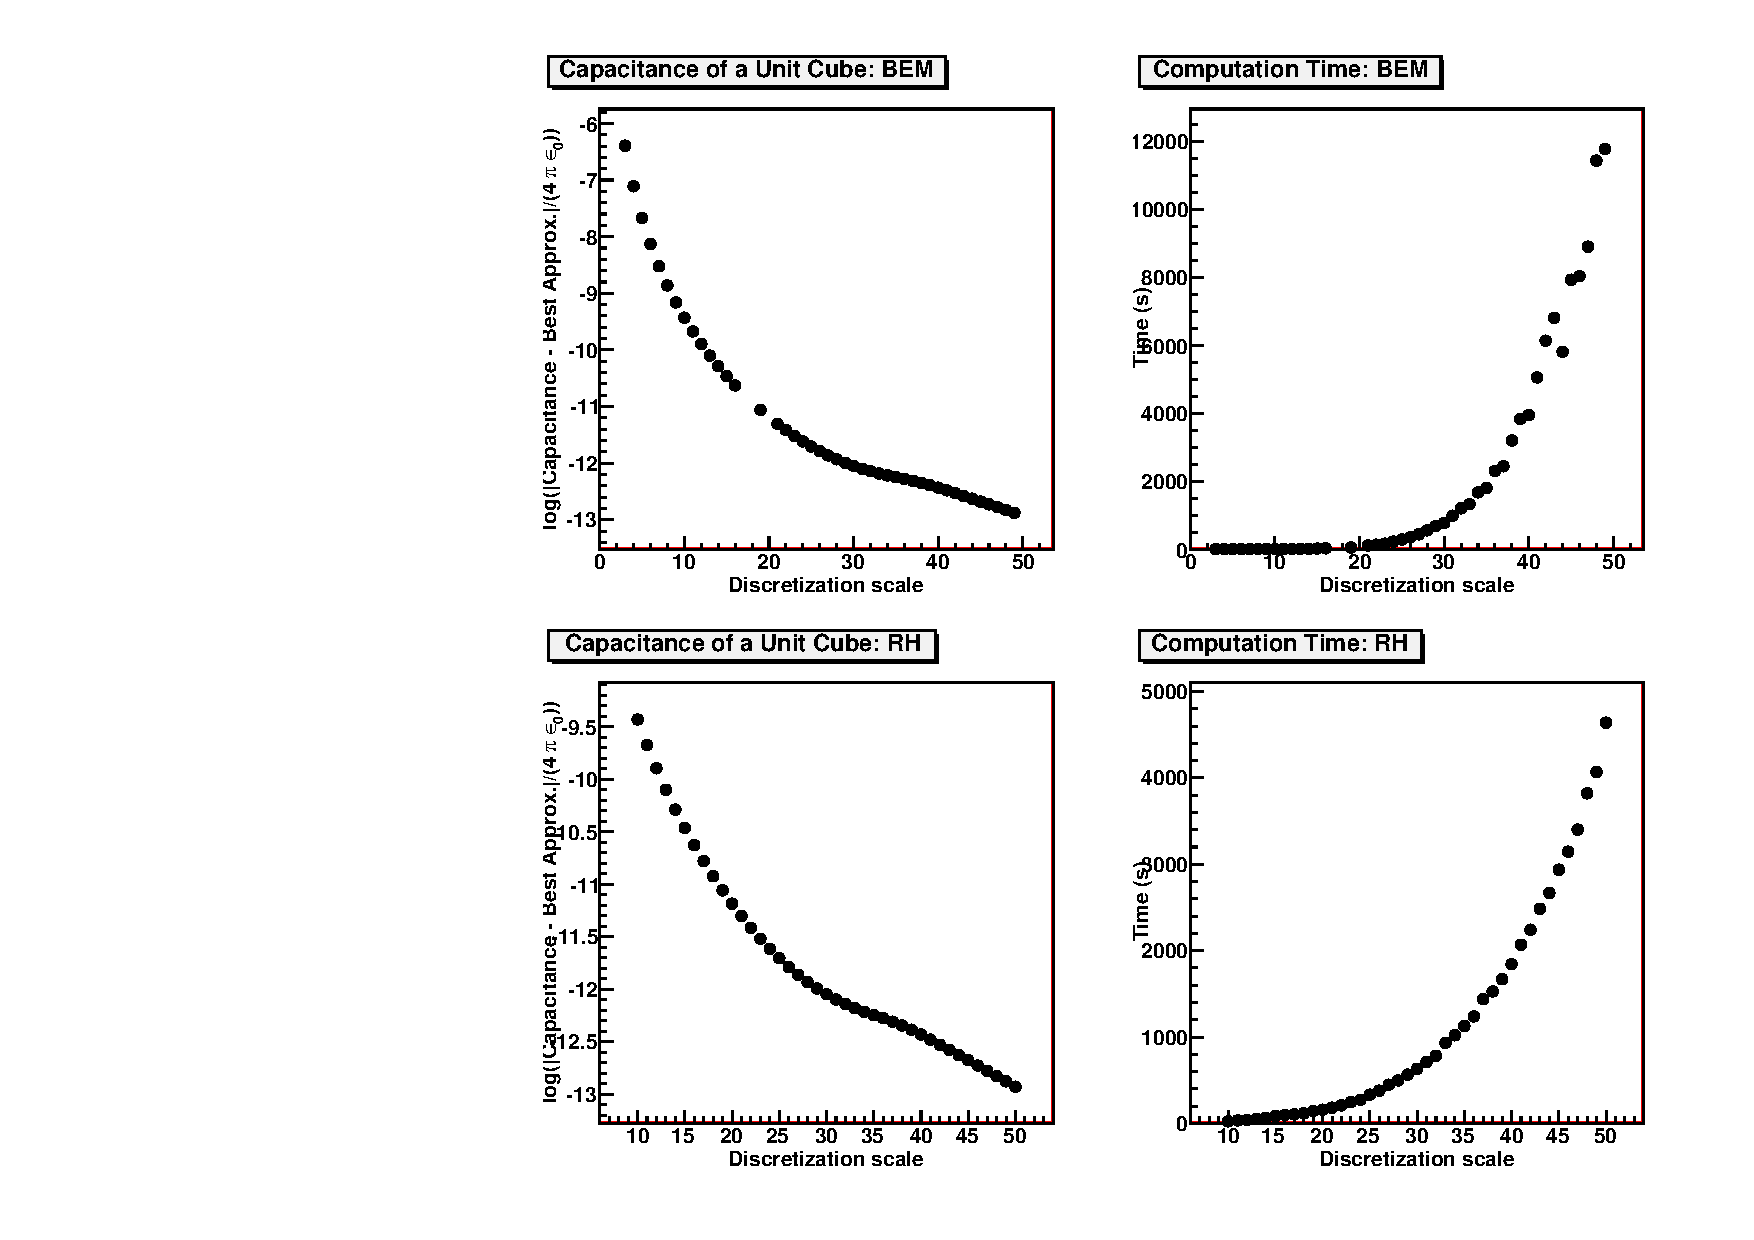
\includegraphics[width=\textwidth]{images/KEMFieldPlots/RH_vs_BEM.pdf}
\caption{Plot of accuracy and computation time for RH and BEM methods as a function of electrode discretization for a unit cube.}
\label{fig:cube_results}
\end{center}
\end{figure}

It is possible to fit the dependance of the accuracy (at least for the unit cube) as a function of iteration.  The following expression...

\begin{equation}
\epsilon \simeq \frac{A}{\sqrt{N}} e^{-\frac{n \tau}{N}}
\end{equation}

\noindent works very well.  Here, $n$ is the iteration number, $N$ is the number of electrodes, and $A$ and $\tau$ are constants.  In the case of the unit cube, $A\simeq 4$ and $\tau \simeq 2.4$, and are fairly independent of the number of electrodes used.  Note that if one assumes that the amount of time ($t$) to compute $n$ iterations depends linearly on $N$ as $t = n N \tau_0$, then one finds...

\begin{equation}
\epsilon \simeq \frac{A}{\sqrt{N}} e^{-\alpha \frac{t}{N^2}}
\end{equation}

\noindent where $\alpha = \frac{\tau}{\tau_0}$ is just a (processor-dependent) constant.  This is consistent with the observation by~\cite{RH1,RH2} that the computation time scales as $N^{1.35}$ for small $N$ and as $N^2$ for large $N$.  The memory footprint however, is always proportional to $N$.

Tests have also been performed on a unit disk with similar convergence behavior.

\subsection{M-Dependence}

The dependence of the convergence on the size of the swap matrix (in this notation, $M$) has also been tested.  The results are shown in Table~\ref{tab:M}.  In general the convergence is best for $M=1$ and gets worse for $M>1$.  Note that $M>1$ for isolated charge cases.

\begin{table}[htdp]
\caption{The convergence dependence on the number of charge exchange electrodes $(M)$ for a test electrode system.  $N$ refers to the total number of electrodes, $n$ is the number of iterations, $t$ is the computation time, and $\epsilon$ is the convergence metric.  In general, the total number of iterations for $M=1$ is greater than $M=2$, but the accuracy is better (for fixed computation time).}
\begin{center}
\begin{tabular}{|c|c|c|c|c|}
\hline
Electrodes & M & Iterations & $\epsilon$ & Time (s) \\ 
\hline
1800 & 1 & 10000 & $5.7 \times 10^{-4}$ & 60 \\
1800 & 2 & 5000 & $1.65 \times 10^{-3}$ & 60 \\
1800 & 6 & 1700 & $9.73\times 10^{-3}$ & 120 \\
\hline
4000 & 1 & 20000 & $1.8 \times 10^{-3}$ & 240 \\
4000 & 2 & 10000 & $2.9 \times 10^{-3}$ & 240 \\
\hline
7200 & 1 & 20000 & $2\times 10^{-1}$ & 360 \\
7200 & 2 & 10000 & $3 \times 10^{-1}$ & 360 \\
\hline
14000 & 1 & 100000 & $9\times 10^{-6}$ & 3600 \\
14000 & 2 & 50000 & $2 \times 10^{-5}$ & 3600 \\
\hline
28000 & 1 & 200000 & $9\times 10^{-6}$ & 21600 \\
28000 & 2 & 100000 & $2 \times 10^{-5}$ & 21600 \\
\hline
\end{tabular}
\end{center}
\label{tab:M}
\end{table}%


\subsubsection{Nested Spheres}

RH has also been tested using two nested metal spheres where the inner sphere held at 10 V while the outer sphere is held at ground (see Fig.~\ref{fig:nested_spheres}).  Gauss' law guarantees that inside the innermost sphere the potential everywhere should be constant (10 V).  Figure~\ref{fig:ns_results} shows the potential sampled from 50,000 points inside the innermost sphere for an accuracy $\epsilon$ of $10^{-1}$ and $10^{-4}$.  Note that the system quickly converges to the correct solution as the requirement on $\epsilon$ is tightened.

\begin{figure}[htbp]
\begin{center}
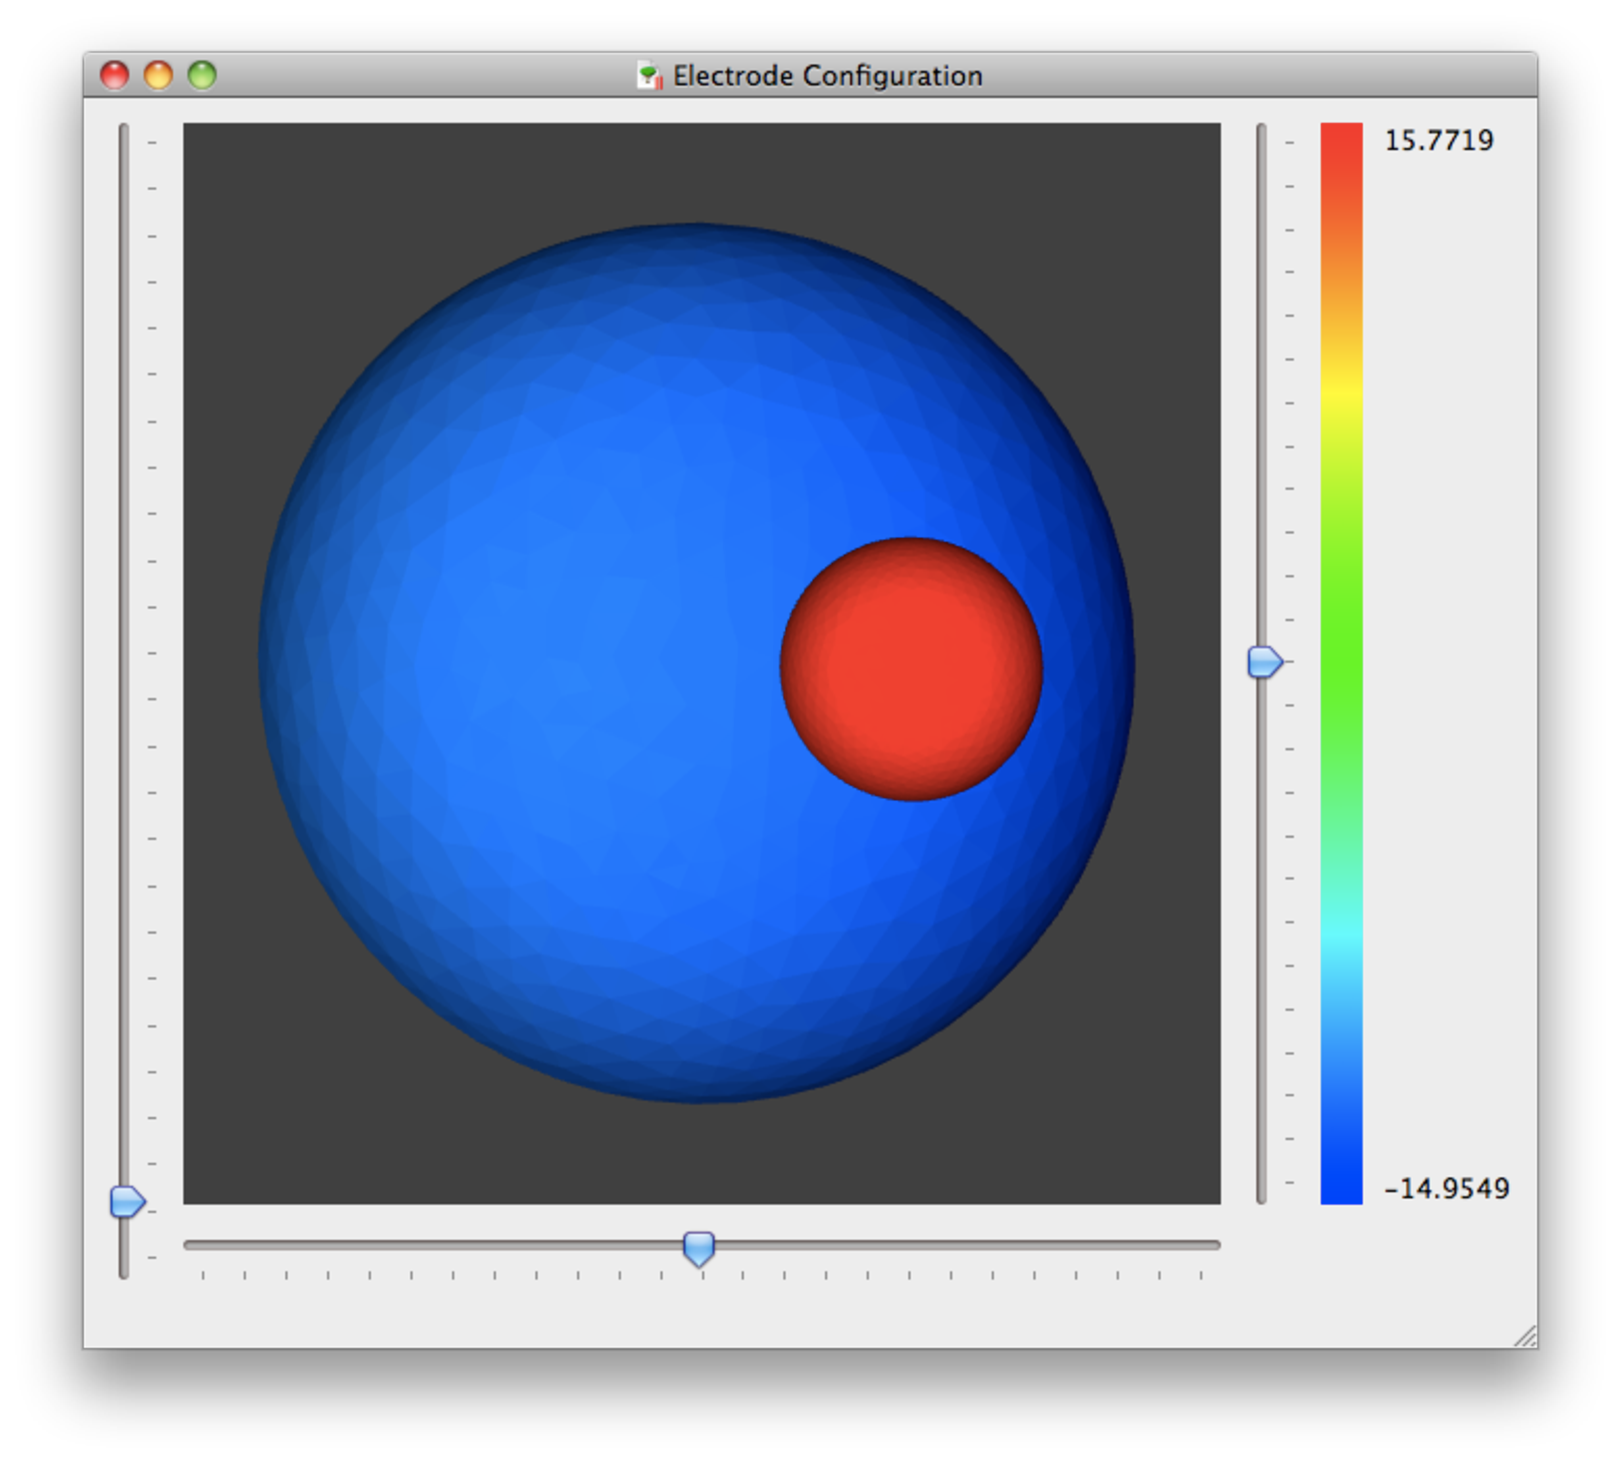
\includegraphics[width=\textwidth]{images/KEMFieldPlots/nestedSpheres.pdf}
\caption{Charge distribution calculated from two nested spheres held at two different potentials.}
\label{fig:nested_spheres}
\end{center}
\end{figure}

\begin{figure}[htbp]
\begin{center}
\begin{tabular}{c c}
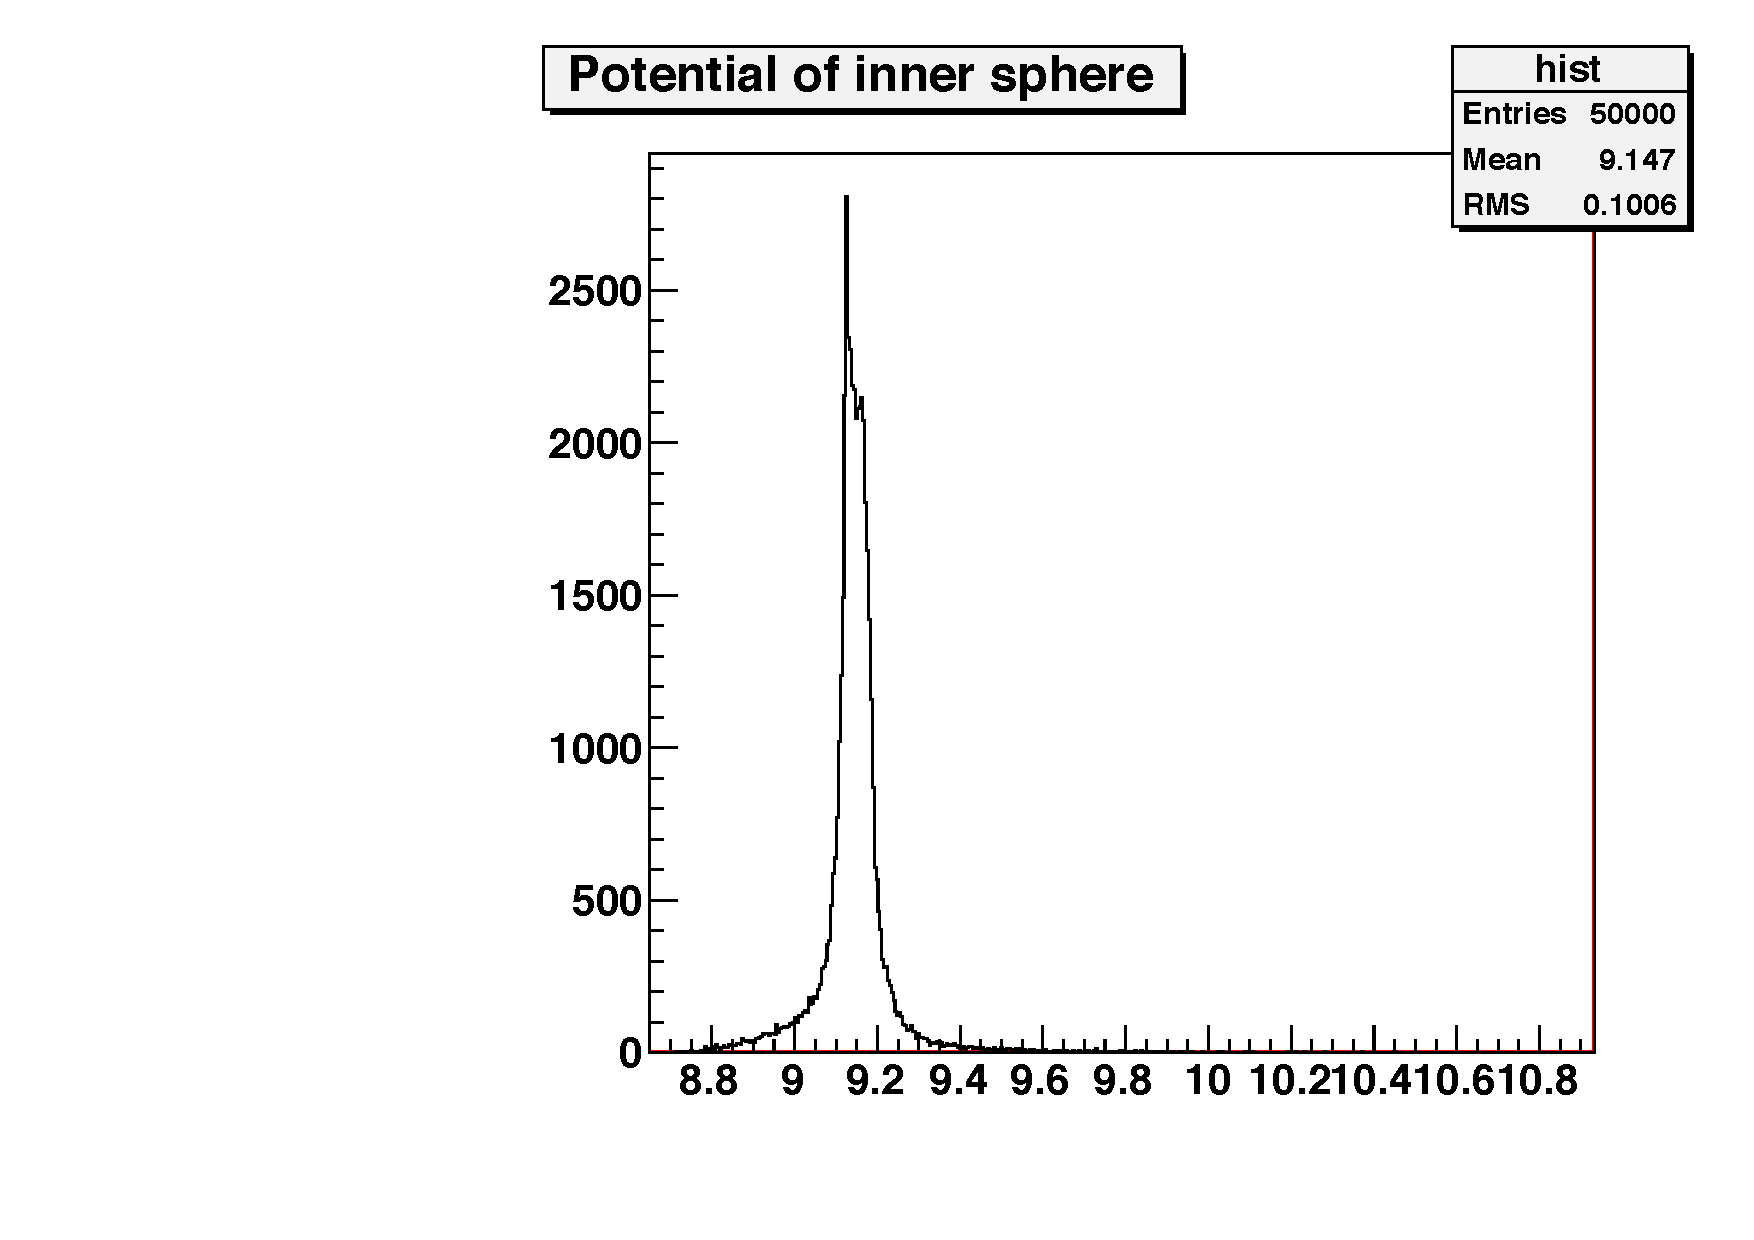
\includegraphics[width=0.5\textwidth]{images/KEMFieldPlots/sphereHist_10e-1.pdf} &
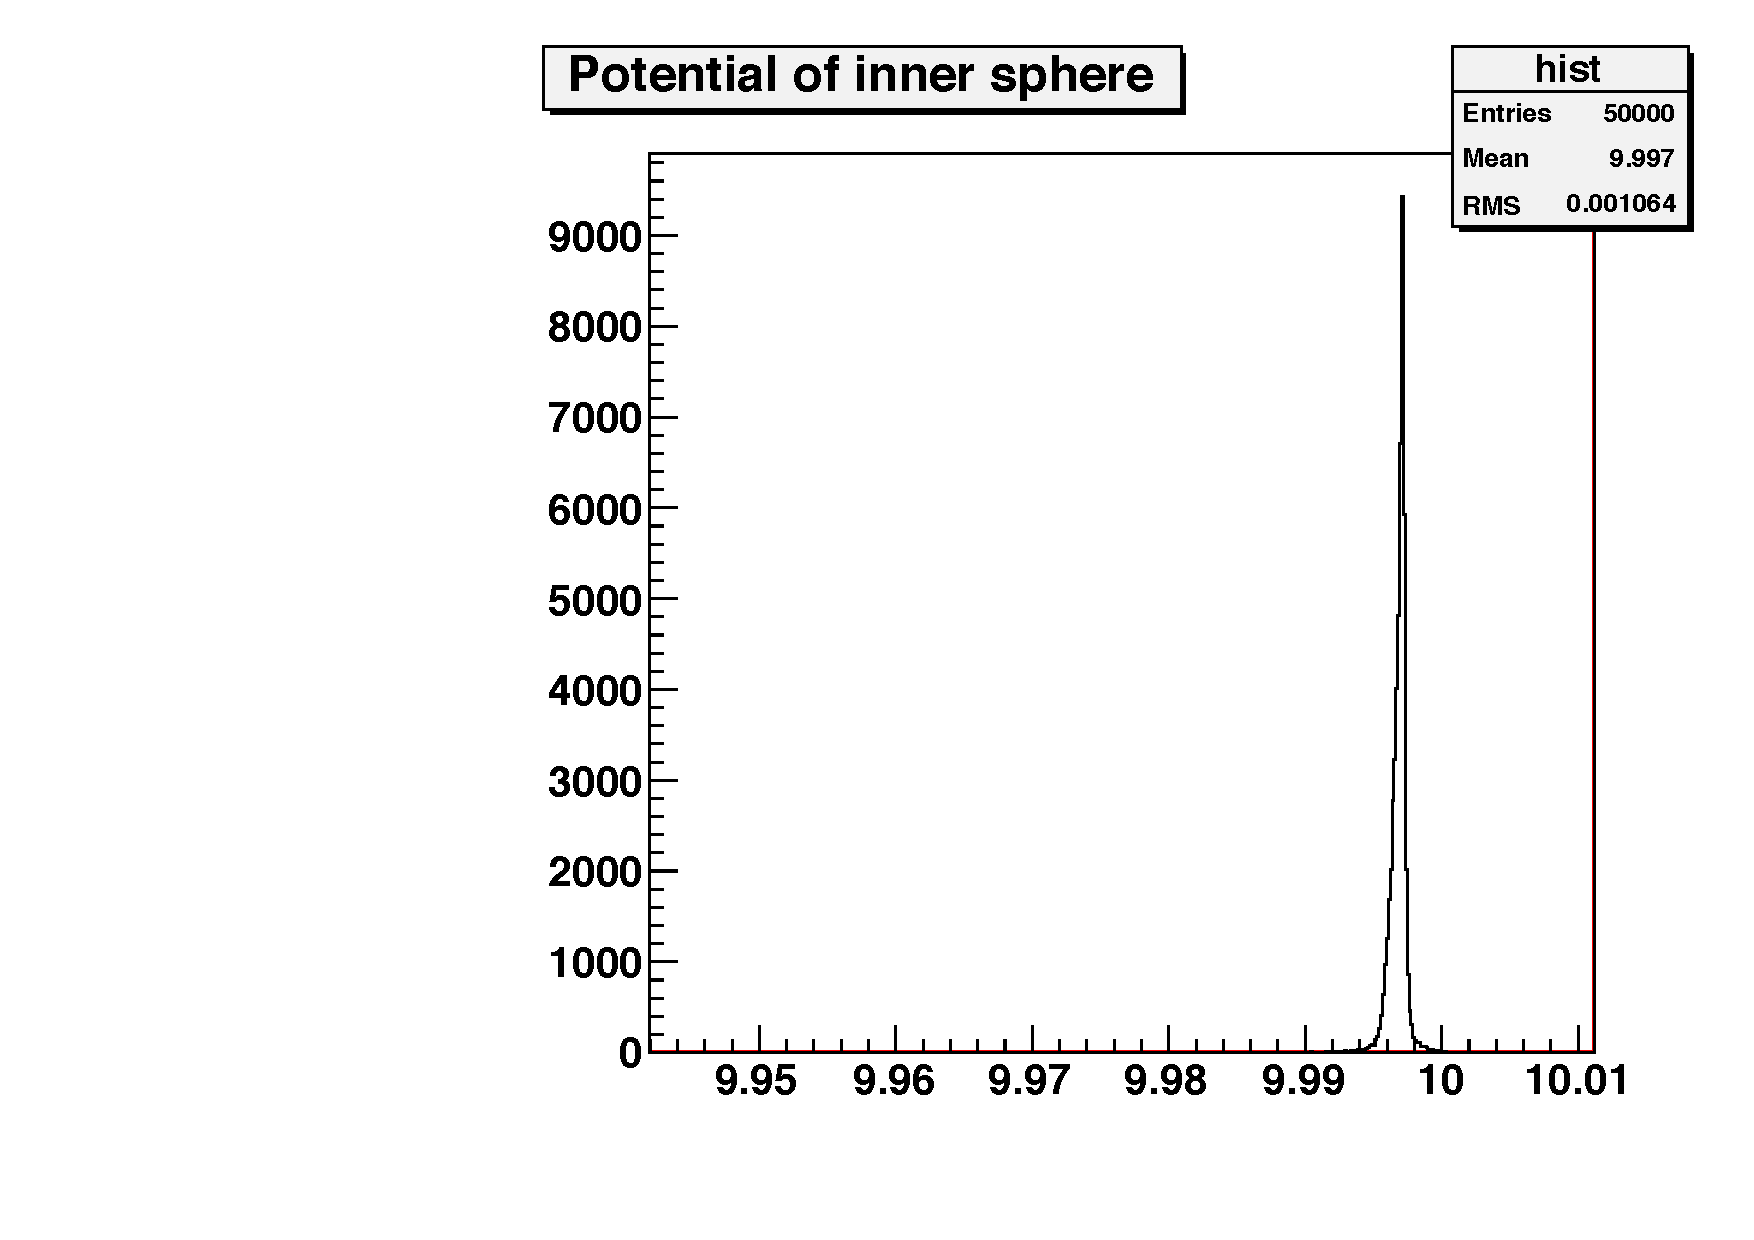
\includegraphics[width=0.5\textwidth]{images/KEMFieldPlots/sphereHist_10e-4.pdf} \\
\end{tabular}
\caption{Potential sampled from inside the smaller nested sphere (at 10 V) for a charge distribution computed from RH with an electrode accuracy requirement of $10^{-1}$ (left) and $10^{-4}$ (right).}
\label{fig:ns_results}
\end{center}
\end{figure}

\subsubsection{Dielectrics}

The Robin Hood method is extremely effective in solving general matrix-inversion equations such as those found in electrostatics, where one effectively solves for the equation...

\begin{equation}
U_i = \sum_{j=1}^N I_{ij} \sigma_j
\end{equation}

\noindent where $U_i$ is the potential of the sub-element $i$, $\sigma_j$ is the charge density of sub-element $j$ of $N$ and $I_{ij}$ is given by...

\begin{equation}
I_{ij} = \frac{1}{4\pi\epsilon_0}\int_{\Delta S_j} \frac{dS_j}{|\vec{r}_i - \vec{r}_j|} 
\end{equation}

The integral expression $I_{ij}$ depends on the distance between point $\vec{r}_i$ and $\vec{r}_j$.  Note that we have implicitly assumed that the surface area $\Delta S_j$ is small enough that the charge distribution within it is constant.

We can expand the Robin Hood method such that it can be used for dielectrics as well.  In the latter case, we need to modify the matrix equation to deal not with potentials (which are fixed at the surface of a conductor) but the boundary conditions imposed by Maxwell's equations~\cite{Rao}.

Therefore, let us take the boundary condition that at the insulator-insulator interface, the displacement vector $\vec{\bf D}$ is continuous across the surface.  This imposes the following condition:

\begin{equation}
\epsilon_i^+ \vec{\bf E}^+_i \cdot \hat{\bf n} - \epsilon_i^- \vec{\bf E}^-_i \cdot \hat{\bf n} = 0
\end{equation} 

\noindent where $\epsilon^{\pm}_i$ is the permittivity above and below the surface of the subelement $i$, $\vec{\bf E}^\pm$ is the electric field, and $\hat{\bf n}$ is the surface normal vector at the insulator-insulator interface at location $i$.  The electric field can be written in integral form as the following...

\begin{equation}
\vec{\bf E}^{\pm}_i = \sum_{j=1}^{N} \frac{\sigma_j}{4\pi\epsilon_0}\int_{\Delta S_j} \frac{(\vec{\bf r}_i - \vec{\bf r}_j)}{|\vec{r}_i - \vec{r}_j|^3} dS_j \pm \hat{\bf n}_i \frac{\sigma_i}{2 \epsilon_0}
\end{equation}

With some manipulation of the above equation, one can re-write the above expression again as a matrix equation.

\begin{equation}
\Psi_i = \sum_{j=1}^{N} \eta_{ij} \sigma_j
\end{equation}

\noindent where for $i\neq j$ we have

\begin{equation}
\eta_{ij} = \frac{1}{4\pi\epsilon_0}\int_{\Delta S_j} \frac{(\vec{\bf r}_i - \vec{\bf r}_j)}{|\vec{r}_i - \vec{r}_j|^3} \cdot \hat{\bf n}_i dS_j
\end{equation}

\noindent and for $i\equiv j$ we have

\begin{equation}
\eta_{ii} = \frac{1}{4\pi\epsilon_0}\frac{2\pi (\epsilon^+_i + \epsilon^-_i)}{\epsilon^+_i - \epsilon^-_i}
\end{equation}

The constraint vector, $\Psi_i$, is simply the null vector.

Formulated in this manner, and taking advantage of the linearity of electric fields, one can impose the same algorithm for solving conductors as one does for insulators.  There exist, however, a few caviats need to be considered.

\begin{enumerate}
\item As this method involves the calculation of the electric field, three components (rather than one) will need to be calculated for each sub-element.
\item This method is well-defined for the case of bound charges from linear media.  For inhomogeneous media, one would need to divide the volume into surfaces and impose the constraint at different depths.
\item Insulators should be treated individually (i.e. no charge exchange between conductors and insulators allowed).
\item Since the system depends on the surface normal $\hat{\bf n}$, one needs to be mindful of the orientation of the surface.
\end{enumerate}

Dielectric media is now implemented in Kassiopeia and has been used in the computation of the fields near the detector region (see Fig.~\ref{fig:detector}).  Preliminary results seem to indicate the method works well.

% KPAGE documentation for the Kassiopeia Guide
%this is a one two one copy from the referenceguide, therefore some links will not work.
%also all changes to be file will be lost, whenever i copy the referenceguide version in here, which is generated by doxygen.
%so save yourself the trouble and edit directly the  original text in  /Modules/Generators/include/PAGEGenerator.h
% because of the different hirarchies, replace subsection with section in here...


\hypertarget{KPAGEmain}{}\section{KPAGE -\/ KATRIN PArticle GEnerator}\label{KPAGEmain}
\begin{DoxyVersion}{Version}
x \hyperlink{_k_p_a_g_emain_KPAGEChangeLog}{ChangeLog} 
\end{DoxyVersion}
\begin{DoxyAuthor}{Author}
wkaefer 
\end{DoxyAuthor}
\begin{DoxyDate}{Date}
2010
\end{DoxyDate}
\begin{DoxyAttention}{Attention}
The source of this documentation can be found in: /Modules/Generators/include/PAGEGenerator.h
\end{DoxyAttention}
\hypertarget{_k_p_a_g_emain_KPAGEIntroduction}{}\subsection{Introduction}\label{_k_p_a_g_emain_KPAGEIntroduction}
KPAGE (Katrin PArticle GEnerator) is the KATRIN standard Particle generator. This document gives a comprehensive overview over KPAGE. Please refer to the class documentations in the reference guide for more details, in particular the physics information.\hypertarget{_k_p_a_g_emain_KPAGEBasicDesign}{}\subsection{Basic Design}\label{_k_p_a_g_emain_KPAGEBasicDesign}
KPAGE provides Particle Generators, which inherit from \hyperlink{class_kassiopeia_1_1_k_s_generator}{KSGenerator} and Creators, which inherit from \hyperlink{class_kassiopeia_1_1_k_s_creator}{KSCreator}. the Creator classes each are responsible for creating one property of a particle, namely position, time, energy, direction. the Generators create a complete particle -\/ either allone, or by combining the creators. Currently, there are only two generators: \begin{DoxyItemize}
\item the \hyperlink{class_kassiopeia_1_1_p_a_g_e_generator}{PAGEGenerator}: this allows to combine different creators to a full generator. Additionally, the user can specify the particle id (note that not all creator classes allow any particle id) and the weight of a generator. \item the \hyperlink{class_kassiopeia_1_1_p_a_g_e_generator_a_s_c_i_i}{PAGEGeneratorASCII}: reads in a textfile and generated particles from that. This generator is completely independent of the creator system. The following creators can be combined in the \hyperlink{class_kassiopeia_1_1_p_a_g_e_generator}{PAGEGenerator}: 
\begin{DoxyItemize}
\item position creators  
\begin{DoxyEnumerate}
\item \hyperlink{class_kassiopeia_1_1_p_a_g_e_position_creator_fix}{PAGEPositionCreatorFix}: 
\item \hyperlink{class_kassiopeia_1_1_p_a_g_e_position_creator_s_s_c}{PAGEPositionCreatorSSC}: 
\item \hyperlink{class_kassiopeia_1_1_p_a_g_e_position_creator_surface}{PAGEPositionCreatorSurface}: 
\item \hyperlink{class_kassiopeia_1_1_p_a_g_e_position_creator_volume}{PAGEPositionCreatorVolume}: 
\end{DoxyEnumerate}
\item time creators  
\begin{DoxyEnumerate}
\item \hyperlink{class_kassiopeia_1_1_p_a_g_e_time_creator_decay}{PAGETimeCreatorDecay}: 
\item PAGETimeCreatorEqual: 
\item \hyperlink{class_kassiopeia_1_1_p_a_g_e_time_creator_fix}{PAGETimeCreatorFix}: 
\end{DoxyEnumerate}
\item energy creators  
\begin{DoxyEnumerate}
\item \hyperlink{class_kassiopeia_1_1_p_a_g_e_energy_creator_equal}{PAGEEnergyCreatorEqual}:  
\item \hyperlink{class_kassiopeia_1_1_p_a_g_e_energy_creator_fix}{PAGEEnergyCreatorFix}:  
\item \hyperlink{class_kassiopeia_1_1_p_a_g_e_energy_creator_gauss}{PAGEEnergyCreatorGauss}:  
\item \hyperlink{class_kassiopeia_1_1_p_a_g_e_energy_creator_krypton}{PAGEEnergyCreatorKrypton}:  
\item \hyperlink{class_kassiopeia_1_1_p_a_g_e_energy_creator_radon}{PAGEEnergyCreatorRadon}:  
\item \hyperlink{class_kassiopeia_1_1_p_a_g_e_energy_creator_tritium}{PAGEEnergyCreatorTritium}:  
\item \hyperlink{class_kassiopeia_1_1_p_a_g_e_energy_creator_tritiumwith_w_g_t_s_energy_loss}{PAGEEnergyCreatorTritiumwithWGTSEnergyLoss}:  
\end{DoxyEnumerate}


\item direction creators  
\begin{DoxyEnumerate}
\item \hyperlink{class_kassiopeia_1_1_p_a_g_e_direction_creator_fix}{PAGEDirectionCreatorFix}: 
\item \hyperlink{class_kassiopeia_1_1_p_a_g_e_direction_creator_gauss}{PAGEDirectionCreatorGauss}: 
\item \hyperlink{class_kassiopeia_1_1_p_a_g_e_direction_creator_isotropic}{PAGEDirectionCreatorIsotropic}: 
\item \hyperlink{class_kassiopeia_1_1_p_a_g_e_direction_creator_surface}{PAGEDirectionCreatorSurface}: 
\end{DoxyEnumerate}
\end{DoxyItemize}\begin{DoxyAttention}{Attention}
Note that while most combinations are allowed, they do not necessarily make sense. And in some cases, the properties depend on each other, in particular, the SurfaceDirectionGenerator only makes sense in combination with a surfacepositioncreator.
\end{DoxyAttention}
\end{DoxyItemize}
\hypertarget{_k_p_a_g_emain_KPAGEusage}{}\subsection{How To Use It}\label{_k_p_a_g_emain_KPAGEusage}
KPAGE's behaviour is fully automatic and determined by the settings in it's option file, so look at that. You can find one in kassiopeias etc directory, it is called GeneratorConfiguration.txt.\hypertarget{_k_p_a_g_emain_KPAGEGenerators}{}\subsection{Generators and Creators}\label{_k_p_a_g_emain_KPAGEGenerators}
\hypertarget{_k_p_a_g_emain_KPAGEIssues}{}\subsection{Known Issues}\label{_k_p_a_g_emain_KPAGEIssues}
the time creators are untested, and the volume creator has been changed... the surface position creator runs in \char`\"{}debug mode\char`\"{}\hypertarget{_k_p_a_g_emain_KPAGEChangeLog}{}\subsection{ChangeLog}\label{_k_p_a_g_emain_KPAGEChangeLog}
\begin{DoxyItemize}
\item 1.0: first version. \item 1.5 more modular layout, allowing to combine position, direction, time and energy creation arbitrarily. \end{DoxyItemize}
\hypertarget{_k_p_a_g_emain_KPAGE_TODO}{}\subsection{KPAGE Todos}\label{_k_p_a_g_emain_KPAGE_TODO}
\begin{DoxyItemize}
\item NOTHING! COOL! \end{DoxyItemize}




% KTrack documentation for the Kassiopeia Guide
\setcounter{secnumdepth}{4}
\section{Particle Tracking: KTrack}\label{sec:KTrack}

KTrack is a program package to compute particle trajectories. The program is valid for any type of particle.

KTrack was developed for simulating the motion of particles in the KATRIN experiment; therefore, the implemented equations of motion describe particle motion in electro magnetic fields. The framework of KTrack, however, allows for implementing an arbitrary equation of motion. 

For solving the equation of motion the user can choose, at present, between six ODE solving methods: \textit{8th order Runge-Kutta}, four different \textit{Emmbedded Runge-Kutta Methods} (\textit{4th/5th order Runge-Kutta}, \textit{5th/6th order Runge-Kutta}, \textit{6th/8th order} and \textit{8th/7th order Runge-Kutta}) and \textit{Predictor-Corrector}. The latter five provide an intrinsic numerical time step control. In addition to these controls, a number of criteria for determining the time step are offered by KTrack. The user can choose to control the step size by means of energy conservation, a global limit on the step size, a fraction of the cyclotron period, limits on the energy loss due to synchrotron radiation, and limits on scattering probability. Any combination of controls can be chosen.

KTrack offers two main computation modes. Firstly, there is an exact trajectory calculation based on solving the Lorentz equation. Secondly, there is a mode which is based on computing the guiding center motion. It makes use of the adiabaticity of the motion, i.e. the conservation of the first order orbital magnetic moment. In this mode magnetron drift motion and gyration are added seperately. A third mode, in which the drift motion is embedded in the equation of motion, will be added in the near future. 
 
The program package also includes elastic and inelastic scattering on hydrogen. Any other scattering module can be added easily. Synchrotron radiation is optionally taken into account in the calculation.

The mathemathical description of the physical processes is taken from Ferenc Gl\"uck's c-language routines.

People involved in developing KTrack:
John Barrett, Daniel Furse, Ferenc Gl\"uck, Wolfgang K\"afer, Benjamin Leiber, Susanne Mertens, Nancy Wandkowsky

\subsection{KTrack's general structure}

In this most recent version, KTrack has been reorganized into a general modular framework.  The basic unit of this framework is called a \textit{Process}, which generally represents any action that changes the state of a particle.  For example, propagating a particle according to an equation of motion using a differential equation solver is a kind of \textit{Process} called, more specifically, \textit{Propagation}, which changes the particle's position and momentum.  The effect of synchrotron radiation loss during a step is likewise encapsulated in a \textit{Process}, called \textit{Synchrotron}.  Its action is to reduce the transverse momentum of a particle.

In addition to the examples above, which are self-contained \textit{Processes} representing specific physics, the \textit{Processes} in KTrack can be combined into composite tree structures.  To give an example, the \textit{Adiabatic Stepping Method} itself is treated as a \textit{Process} in KTrack, and it sits at the base of a tree whose branches represent sub-\textit{Processes}.  In the case of the \textit{Adiabatic Stepping Method}, these branches are a \textit{Propagation Process}, possibly a \textit{Synchrotron Process}, possibly a \textit{Drift Process}, a \textit{Gyration Process}, and finally, possibly a \textit{Scattering Process}.  This tree-like structure is realized in C++ according to the \textit{Composite} pattern, described in \ref{compsite}.

As mentioned above, there are various criteria to control the step size available in KTrack.  The basic behavior of these controls is captured in a class called \textit{StepSize}, and each step size naturally belongs to a particular \textit{Process}.  For instance, the energy conservation step control naturally belongs to \textit{Propagation}, and the synchrotron radiation step size control naturally belongs to \textit{Synchrotron}.  Each of these controls is able to suggest a time step, which is that control's best guess at the maximum time step it itself can tolerate.  Each control is also able to examine whether the action of its parent process has exceeded the control's tolerance, at which point it can veto the step and make an improved suggestion for the step size.

The methods of all classes can be classified as following types:
\begin{itemize}
    \item action: 
        \begin{itemize}
            \item initialize processes
            \item changing the state of the particle
            \item reset processes
            \item compute time step
        \end{itemize}
    \item composition       
        \begin{itemize}
            \item add processes/step size controls
            \item remove processes/step size controls
            \item get processes/step size controls
        \end{itemize}
    \item identification
        \begin{itemize}
            \item get name of class
            \item get type of class
            \item get name of parent class
        \end{itemize}
    \item configuration
        \begin{itemize}
            \item set parameters
            \item set field calculation method
            \item set cross section calculation method
            \item etc.
        \end{itemize}
    \item delegation:  methods called by child process to get information about the parent process 
        \begin{itemize}
            \item e.g. returns pointer to the ODE that is used
            \item e.g. returns pointer to intermediate particle
            \item etc.
        \end{itemize}
\end{itemize}

Further technical details and discussion of how the tree-like structures of \textit{Processes} are composed; how \textit{StepSizes} are attached and configured, and how initialization generally occurs within such structures can be found in the following chapters.

\subsection{KTrack Step Computer}
\label{ktrackstep}  

A \textit{KTrack Step Computer} is itself of the type \textit{Process}; the class \textit{KTrackStepComputer} inherits from \textit{Process}. A full step is composed of a number of sub processes. To perform a step \textit{KTrack Step Computer} has the following public method:
    \begin{itemize}
        \item Execute()
    \end{itemize}
    To organize sub processes \textit{KTrack Step Computer} has the following public methods:
    \begin{itemize}
        \item AddProcess(*process)
        \item RemoveProcess(std::string processname)
        \item GetProcess(std::string processname)
    \end{itemize}
    KTrack has two tracking methods, so far, the exact and adiabatic method, (these are described in more detail below, see \ref{exactadiabatic}). The corresponding classes \textit{ExactStep} and \textit{AdiabaticStep} inherit from the base class \textit{KTrackStepComputer}. As a private member, they have a vector of pointers to the processes that are activated by the user.
    
    When calling \textit{Execute()} on an exact or adiabatic step object following actions take place:
      \begin{itemize}
        \item Check whether the current step is the first step of a track:
        \begin{itemize}
            \item If yes: initialize intermediate particles (see \ref{intermediate particles}) and ODE
            \item If no: use the final state of the particle from the step before
        \end{itemize}
        \item Do while:
        \begin{itemize}
            \item compute the time step: ask the \textit{StepSizeOrganizer} to return the smallest suggestion of a time step from all activated step size controlers (see \ref{stepsizes}) 
            \item execute all activated processes: call \textit{Execute()} on all processes of the vector of processes in the right order. If the execution fails the step size control that failed reduces the time step and the program continues at the beginning of the while loop.
        \end{itemize} 
        \item Update intermediate and basic particle (see \ref{intermediateparticle})
      \end{itemize} 
        
    By calling \textit{AddProcess(*Process)} the process given in the argument is added to the vector of processes. This allows for switching on a process (e.g. scattering) in a certain region. It checks whether this process can be added, i.e. it checks if the process is applicable for the chosen stepping method - one could not add \textit{Drift} to the exact stepping method - and whether this process has already been added. It also takes care of the ordering of the processes, by putting the process in the right position of the vector of processes. To realize the ordering, the entires of the vector are couples of pointers to the \textit{processes} and a string, that describes with process is allowed to be at this position. 
    
    \textit{RemoveProcess(std::string processname)} removes a process from the vector. \textit{GetProcess(std::string processname)} returns a pointer to an object with the corresponding process name. With the help of this method, one can change the settings of the processes during run time.
    
    
    \subsubsection*{Exact and adiabatic stepping method}
    \label{exactadiabatic}   
    As mentioned, KTrack has two different stepping methods. One method, called \textit{Exact Stepping Method}, computes the exact trajectory, by solving the Lorentz equation. The other one, called \textit{Adiabatic Stepping Method}, computes the guiding center motion of the particle and adds the gyration in as a separate \textit{Process}. Here, the magnetron drift of the particle can optionally be swiched on. Both methods offer the possibilty to take synchrotron radiation and scattering processes into account. The adiabatic method has the potential to be much faster compared to the exact method, since it allows for much larger step sizes.
    
    Technically, there are only three differences between the adiabatic and exact stepping method:
    \begin{itemize}
         \item The ordered set of sub-processes is different: 
         \begin{itemize}
             \item In the case of the exact stepping method the only possible processes are: \textit{Propagation}, \textit{Synchrotron} and \textit{Scattering}. 
             \item For the adiabatic stepping method \textit{Propagation}, \textit{Drift}, \textit{Synchrotron}, \textit{Gyration}, and \textit{Scattering} are possible.
         \end{itemize} 
         \item Exact step and adiabatic step work with the so-called \textit{Exact Step Particle} and the \textit{Adiabatic Step Particle}, respectively. See chapter \ref{intermediateparticle}.
        \item Different ODEs are used in the process \textit{Propagation}:
        \begin{itemize}
            \item \textit{Exact Stepping Method} uses the Lorentz equation: 
                \begin{eqnarray}
                    \dot {\vec{x}} &=& \vec{v} \\
                    \dot {\vec{v}} &=& q \left(\vec{E} + \vec{v} \times \vec{B} \right) 
                \end{eqnarray} 
            \item \textit{Adiabatic Stepping Method} uses:
                \begin{eqnarray}
                    \dot {\vec{x}} &=& \hat{B} v_{\mathrm{long}} \\
                    \dot {v}_{\mathrm{long}} &=& -\frac{\mu}{\gamma} \left(\vec{\nabla} |\vec{B}| \right) \hat{B} + q \vec{E} \cdot \hat{B}
                \end{eqnarray} 
        \end{itemize}
        
    \end{itemize}  

\subsection{Processes}
\label{processes}
A step is composed of a number of \textit{Processes}:
\begin{itemize}
\label{listofprocesses}
    \item Propagation
    \item Synchroton radiation
    \item Elastic and inelastic scattering processes
    \item Magnetron drift motion (only needed for adiabatic stepping method)
    \item Gyration motion (only needed for adiabatic stepping method)
\end{itemize} 

The processes are structured in a common way. This is reflected by the fact that they all inheret from the common base class \textit{Process.h}. All processes share the method \textit{Execute()} which performes the required calculations and updates the affected particle properties.

In both the adiabatic and exact KTrack mode (see \ref{modes}) a step begins with the \textit{Propagation}. After the propagation, \textit{Synchroton} radiation is executed. In the case of the adiabatic method the \textit{Drift} (optionally) and \textit{Gyration} are executed afterwards. Finally \textit{Scattering} is executed. 

The set of \textit{Processes} can be divided into two man subsets. One is the \textit{Propagation}, performed by solving an equation of motion. The other \textit{Processes}, such as \textit{Synchrotron Radiation}, \textit{Scattering}, \textit{Magnetron Drift Motion} and \textit{Gyration Motion} are treated as corrections to the \textit{Propagation}.  They actually take place during the propagation, however, in the code they are added after the propagation has already been performed. To reflect reality best, these processes need information about the state of the particle at the beginning (initial particle) and at the end of the propagation (final particle), in order to compute quantities like energy loss due to synchrotron radion or scattering probability, from averaged initial and final particle properties. To allow for that, all processes have the methods \textit{SetInitialParticle()} and \textit{SetFinalParticle()}. 

The general \textit{KTrack Step Computer} is also of the type \textit{Process}. Calling \textit{Execute()} executes all processes that are activated by the user, in the right order. In addition the \textit{KTrack Step Computer} has methods, for adding, removing and returning processes: \textit{AddProcess()}, \textit{GetProcess(std::string name)}, \textit{RemoveProcess(std::string name)}. These methods allow for switching on and off and adjusting different kind of processes during run time.

The process class also offers the possibiliy to ask the name of a process, by calling \textit{GetName()}. Calling \textit{GetName()} on the \textit{KTrack Step Computer} returns which type of stepping is used, i.e. adiabatic or exact stepping method. 

The process \textit{Propagation} additionally includes the methods to set a particular method to solve ordinary differential equations and magnetic and electric field calculation methods: (\textit{SetODESolver()}, \textit{SetMagneticFieldCalculator()}, \textit{SetElectricFieldCalculator()}).
          
          
    \subsubsection*{Propagation}
    The \textit{Propagation} classes in KTrack are responsible for moving a particle along in time according to a step computer's equation of motion.  There are two types of propagation used in KTrack.  The general type, simply called \textit{Propagation} can make use of any ODE solver in KMath; the other, called \textit{ErrorPropagation}, is exclusively for use with ODE solvers that can estimate internally the numeric errors suffered in making a step.
    
The \textit{Propagation} encapsulates the method used for solving the equation of motion, hiding the chosen strategy (RK8, RK86, PC) from the \textit{Step Computer}.  

    In contrast with other \textit{Processes} in KTrack, \textit{Propagation} can accept and manage a number of step size controllers itself.  All \textit{Propagation} classes can accept the \textit{StepSize} controllers for energy conservation, cyclotron period fraction, and constant length.  However, only the \textit{ErrorPropagation} class can accept the \textit{StepSizeNumeric} controller that enables the ODE solver to suggest its own next time step.  For both \textit{Propagation} classes, when asked for a step suggestion, the smallest suggestion of all the installed \textit{StepSize} classes is returned.  Likewise, the \textit{Execute()} function will only return true if all installed step size controllers return true. 
    
    Basically, the task of the \textit{Propagation} classes is to convert the state of the \textit{StepComputer}'s particle to the initial conditions of the ODE, represented by an array of doubles. It operates on that array using the ODE solver initialized with the \textit{StepComputer}'s ODE, and then finally uses the resulting array of doubles from the ODE solver to update the state of the \textit{StepComputer}'s particle.  This operation on arrays of doubles representing the particle's state is a result of the architecture of the \textit{KMathODE} and \textit{KMathODESolver}, discussed below.
    
    By the fact that the only \textit{Process} aware of the full type of the ODE and Particle is the \textit{StepComputer} itself, upon initialization, the \textit{Propagation} class gets the blocks for the ODE initial and final conditions from the \textit{StepComputer}, using the functions \textit{Double\_t* GetInitialConditionBlock()} and \textit{Double\_t* GetFinalConditionBlock()}.  Once these blocks are obtained, \textit{Propagation} operates on them with its ODE solver, finally calling the function \textit{void UpdateFinalParticleFromFinalCondition()} to update the \textit{StepComputer}'s final particle.  
         
        \textbf{ODE:}\\
        The \textit{KMathODE} architecture is quite simple, in order to make it as efficient as possible.  The ODE takes a pointer to a block of doubles from which it reads its initial conditions (via the \textit{SetInitialConditionBlock(Double\_t*)} function), and a pointer to a block of doubles to which it writes its final conditions (via the \textit{SetFinalConditionBlock(Double\_t*)} function).  Whenever the command \textit{Evaluate()} is called on the ODE, the initial conditions are read, and the results of the calculation are written to the final condition area. In order to optimize speed, no checking whatsoever is performed on the sizes of the arrays passed to the ODE, so appropriate caution should be followed when ever making a new class that uses these classes.
        
        There are two ODEs used in KTrack; one in the \textit{AdiabaticStep} class and one in the \textit{ExactStep} class.  These equations are fully given in section \ref{exactadiabatic}).

        \textbf{ODE Solver:}\\         
        The architecture of the \textit{KMathODESolver} is very similar to that of the \textit{KMathODE}.  To use it, one also sets blocks of doubles from which the initial conditions read and to which the final conditions will be written.  Following this, one sets a pointer to a \textit{KMathODE} which lets the \textit{KMathODESolver} initialize its internal storage areas to suit the dimension of the ODE.  Finally, one can call the function \textit{Solve(Double\_t)}, where the argument is a time step.
        
        For the case of the \textit{KMathODEErrorSolver}, the interface is extended to include setting pointer blocks where component-by-component error tolerances can be specified, using the functions \textit{void SetMinErrorConditionBlock(Double\_t*)} and \textit{void SetMaxErrorConditionBlock(Double\_t*)}. I.e. in the case of the Lorentz equation the user might specify an error on each component of the position and the momentum.  
         
        Also, the user can retrieve the calculated step validity via the function \textit{Check()}, as well as the suggested next time step via the function \textit{ComputeTimeStep()}.  It is this extended functionality that is harnessed by the class \textit{StepSizeNumerical}, providing user access to the internal configurability of \textit{KMathODEErrorSolve} without exposing it directly.
        
        There are three ODE solution methods currently used in KTrack, as follows:
        
        \begin{itemize}
            \item \textit{KMathRK8}:  This is a straightforward, 8th order Runge-Kutta integrator requiring 13 evaluations per step\cite{RK8}.
            \item \textit{KMathRK86}:  This is an 8th order Runge-Kutta integrator requiring 12 evaluations per step, with an embedded 6th order integrator inside\cite{Barrett2010}.  This solver is capable of estimating numerical errors. (Other embedded RK-methods will be implemented soon)            
            \item \textit{KMathPredictorCorrector}:  This is an Adams-Bashforth predictor utilizing a modified Adams-Moulton corrector requiring 2 evaluations per step\cite{Faust2008}.  This solver is capable of estimating numerical errors.  
        \end{itemize}

        
    \subsubsection*{Synchrotron}
    Optionally, at the beginning of executing \textit{Synchrotron Process}, \textit{Check()} in \textit{StepSizeSynchrotron} is called, to check whether the maximal energy loss was exceeded. If not, the particle's transverse momentum is updated. 
    
    Synchroton radiation is computed from the initial and final particle properties 
    \begin{equation}
        \frac{E_{\mathrm{loss}}}{E_{\mathrm{kin}}} = x_{\mathrm{enh}} c_{\mathrm{magic}} \langle \gamma \rangle \langle \vec{B}^2 \rangle \cdot \Delta t,
    \end{equation}
        where $x_{\mathrm{enh}}$ is the synchrotron radiation enhancement factor, given by the user, $c_{magic}$ is a magic number of 0.3877, which falls from heaven, $\langle \gamma \rangle$  is the average lorentz factor, $\langle \vec{B}^2 \rangle$ is the average magnetic field squared.
        The new transverse momentum is given by:
    \begin{equation}
        p_{\mathrm{trans,new}} = \sqrt{p_{\mathrm{trans}}^2 (1 - \frac{E_{\mathrm{loss}}}{E_{\mathrm{kin}}})}
    \end{equation}  
    At the end of the execution, the final particle's transverse momentum is set to the new value. 
    
    \subsubsection*{Scattering}
    At the start of executing \textit{Scattering Process}, it is checked whether the step exceed the maximal allowed scattering probability. If not, scattering is performed. 
    
    The  architecture of the scattering classes follows the same composite structure as the rest of KTrack: there is a purely virtual base class called \textit{ScatteringModule}, which inherits from \textit{Process}. The following classes inherit from this base class:
    \begin{itemize}
        \item Scattering
        \item SingleSpeciesScattering 
	\begin{itemize}
		\item Hydrogen
		\item Argon
		\item Nitrogen
		\item Water
	\end{itemize}
        \item SingleSpeciesElastic, SingleSpeciesIonization, SingleSpeciesExcitation
    \end{itemize}
    When calling \textit{Execute()} on an object of the class \textit{Scattering}, it decides whether scattering takes place at all. If so, it decides on which module (i.e. scattering on hydrogen or any other activated molecule). Then \textit{Execute()} is called on the active module. Within this method, the module decides which kind of scattering actually takes place (i.e. elastic, ionization, excitation). Once that is decided, \textit{Execute()} is called on the specific submodule. There, the energy loss and the angle change are computed and the particle is correspondingly updated. The classes \textit{Scattering} and \textit{SinleSpeciesScattering} have methods \textit{Add- Remove- and Get-Process}, as any parent \textit{Process} class. This allows for adding scattering modules and submodules and adjusting their parameters during run time. This structure is designed in a way that extending the code in the future to use more scattering modules is very easy.
    
    The modules \textit{SingleSpeciesScattering} have a pointer to a density calculator, which can be a calculator that returns a constant value, or a calculator that has a connection to SSC (Source Spectrum Calculation) and returns a density depending on the position. This is not fully implemented, yet.
    
    The submodules (e.g. \textit{SingleSpeciesElastic}) have a pointer to a basic calculator which performs the actual computation of cross sections, the energy loss, and the change of the angle.
    
    So far only a basic calculator bases on scattering on $H_2$ is available. These calculators use original Ferenc Gl\"uck's c-language routines. Details about these calculations can be found in the \textit{KScattering} directory.
        
    \subsubsection*{Drift}
    This process has no initial check. The drift velocity is computed in the following way:
    \begin{eqnarray}
    {v}_{\vec{\nabla} \times \vec{B}} &=& \left \langle \left( \frac{ \gamma m }{ q  |B|  ^3} \frac{  v_{\mathrm{long}}^2  v_{\mathrm{trans}}^2 }{2} \right) \vec{B} \times \nabla  |\vec{B}| \right \rangle \\
    \vec{v}_{\vec{E} \times \vec{B}} &=& \left \langle \vec{E} \times  \vec{B} \left(\frac{1}{ \vec{B}^2}\right) \right \rangle \\
    \vec{v}_{\mathrm{drift}} &=& \vec{v}_{\vec{\nabla} \times \vec{B}}  + \vec{v}_{\vec{E} \times \vec{B}}
    \end{eqnarray}
    At the end of the execution of the drift, the final particle's position is updated, according to
    \begin{equation}
        \vec{v}_{\mathrm{drift}} dt = \Delta \vec{x}
    \end{equation} 
    
    
    \subsubsection*{Gyration}
    This process has also no initial check. 
    
    The mathematical description of the gyration is the following: In the beginning of a track the guiding center is computed by these equations:
    \begin{eqnarray}
        \vec{r}_{\mathrm{gc}} &=& \vec{r}_{p} - \frac{p_{\mathrm{trans}} \hat{r}_{\mathrm{gc\rightarrow p}}}{q |\vec{B}(\vec{r}_{\mathrm{gc}})| }\\
        \hat{r}_{\mathrm{gc\rightarrow p, orth}}  &=& \hat{B} \times \hat{r}_{\mathrm{gc\rightarrow p}} \\
    \end{eqnarray}
    
    After the step the real particle position is computed from temporary $\hat{r}_{\mathrm{gc\rightarrow p}}$ and $\hat{r}_{\mathrm{gc\rightarrow p, orth}}$ vectors, that correspond to a motion of the particle without torsion. The new $\hat{r}_{\mathrm{gc\rightarrow p}}$ is a linear combination of the two temporary vectors: 
    \begin{eqnarray}
        \hat{r}_{\mathrm{gc\rightarrow p, temp}} &=& \hat{r}_{\mathrm{gc\rightarrow p, orth}} \times \vec{B}(\vec{r}_{\mathrm{gc}}) \\
        \hat{r}_{\mathrm{gc\rightarrow p, orth, temp}}  &=& \hat{B}(\vec{r}_{\mathrm{gc}}) \times \hat{r}_{\mathrm{gc\rightarrow p, temp}} \\
        \hat{r}_{\mathrm{gc\rightarrow p, new}}  &=& \cos(\alpha) \hat{r}_{\mathrm{gc\rightarrow p, temp}} + \sin(\alpha) \hat{r}_{\mathrm{gc\rightarrow p,orth, temp}} \\
        \vec{r}_{p} &=& \vec{r}_{\mathrm{gc}} + R_{\mathrm{gyration}} \hat{r}_{\mathrm{gc\rightarrow p, new}}
    \end{eqnarray}
    
    The cyclotron phase $\alpha$ is given by following eqation:
    \begin{equation}
        \alpha = - 2 \pi \frac{q}{|q|} \langle f \rangle t
    \end{equation}
    
    Within \textit{Execute()} the following steps are performed:
    \begin{enumerate}
        \item A new temporary vector pointing from the guiding center to the real particle position is computed. This temporary vector is set to be the new final particles $\vec{r}_{gc\rightarrow p}$. 
        \item The cyclotron phase is computed, i.e. the change of the azimuthal angle
        \item The real new vector pointing from the guiding center to the real particle position is computed
	    \item Finally, the final particle's vector pointing from guiding center to particle position is updated to the new value.
    \end{enumerate}

\subsection{Step size control}
\label{stepsizes}
At the beginning of a step, it must decided which time step to take. For this purpose KTrack uses a number step size criteria:
\begin {itemize}
    \item maximal numerical error
    \item maximal energy conservation violation
    \item maximal allowed step length
    \item maximal fraction of cyclotron period
    \item maximal allowed energy loss due to synchrotron radiation
    \item maximal allowed scattering probability
\end {itemize}
All these step size controls can be independently used and adjusted by the user. 

The step size control system has two main tasks, the \textit{Suggestion} and the \textit{Check}. In the beginning of a step all active step size controllers are asked to suggest a time step. This is handled by the \textit{StepSizeOrganizer}, that has a vector of pointers to all active step size controllers.

The \textit{Propagation} will be performed with the smallest of all suggestions. At the end of executing the propagation, a sub set of step size controllers, the \textit{Propagation based step controls} are asked to check whether this step exceeds any of the given limits. (E.g. if the violation of energy conservation was really within the allowed range). If one of the checks fails, the step is repeated with a smaller time step. This is repeated until all checks are successful. 

For the processes \textit{Synchrotron} and \textit{Scattering}, the ordering is different. At the beginning of executing these processes, it is checked whether the step taken does not exceed any limits, (i.e. synchrotron radiation not too large, scattering probability not too high). If so, the process \textit{Synchrotron} and \textit{Scattering}, respectively, is applied. In the case the check fails, the process \textit{Propagation} is repeated with a smaller time step, which is suggested from whichever step controller failed. The processes \textit{Drift} and \textit{Gyration} are not controlled by a step controler, so far.

The following sections will expain how the step controllers suggest time steps and how they alter their suggestion in case the check fails.
 

    \subsubsection*{Propagation based step control}
    Propagation-based step controls are used within the execution of the \textit{Propagation}.
        
        \textbf{Energy conservation:}\\
        The suggested time step for the first step can not be determined by means of energy conservation. Therefore, the first suggestion is the cyclotron period. 
        The user can specify an interval, in which the error of the energy conservation violation is permitted. At the end of the execution, \textit{$StepSizePropagation\rightarrow Check()$} is called. 
        \begin{itemize}
            \item If the error is smaller than the lower bound, the step is taken (\textit{Check()} returns true), but the next suggestion of the time step will be multiplied by $1.5$
            \item If the error is within the allowed range, the step is taken (\textit{Check()} returns true); the next suggestion of a time step will be the same as for the step before.
            \item If the error is larger than the upper bound, the step must be repeated (\textit{Check()} returns false) with a time step that is reduced by a factor of $\frac{2}{5}$.
        \end{itemize}
        
        \textbf{Maximal path length:}\\
        The suggested time step is the following:
        \begin{equation}
            t_{\mathrm{suggestion}} = \frac{l_{\mathrm{max}}}{v_{\mathrm{initial}}} 
        \end{equation}
        If the particle is accelerated during the step, the actual step length taken will exceed the upper bound given by the user. Therefore, the step has to be repeated with a smaller time step:
        \begin{equation}
            t_{\mathrm{suggestion,new}} = \frac{l_{\mathrm{max}}}{\frac{v_{\mathrm{initial}}+v_{\mathrm{final}}}{2}} 
        \end{equation}
        
        \textbf{Fraction of cyclotron period}\\
        The suggested time step is given by following equation:
        \begin{equation}
            t_{\mathrm{suggestion}} = \frac{1}{x_{\mathrm{usergiven}} f_{\mathrm{initial}}},
        \end{equation}
        where $x_{\mathrm{usergiven}}$ is the specified cyclotron fraction and $f$ the cyclotron frequency.
        Since the step size classes have access to the intermediate particle, the cyclotron frequency is directly returned from the particle.
        In the actual implementation, this step size is not checked. It would be, however, more consistent to check whether after one step the time step did not exceed the user given fraction of a cyclotron period. The correction of the suggestion would be calculated from the average cyclotron frequency. (To be discussed with Ferenc).
        
        \textbf{Numerical error:}\\
        The numerical error step size control can only be used if \textit{RK86} or \textit{PredictorCorrector} is chosen as ODE solver. Differing from all other step size controllers, the time step is computed within the ODE solver itself. 
        
         The suggested time step for the first step can not be determined by means of f the numerical error. Therefore, the first suggestion is the cyclotron period. 
        
        The user can specify an interval, in which the numerical error is permitted. At the end of executing propagation:
        \begin{itemize}
            \item If the error is smaller than the lower bound, the step is taken. The improved suggestion for the next time step is
            \begin{itemize}
                \item Embedded RK86: 
                %\begin{equation}
                %    t_{suggestion, new} = \min\limits_{i} \{ \left|\frac{1}{\frac{e_{num_i}}{e_{user,min,i}}|}\right| ^{\frac{1}{8}} t_{old} \}, i = (1...\# variables) 
                %\end{equation} 
                \begin{equation}
                    t_{\mathrm{suggestion, new}} =  \min \limits_{i} \left \{ \left|  \frac{ E_{\mathrm{user_i}} }{ E_{\mathrm{num_i}} } \right |^{1/7 } \right \} \times t_{\mathrm{old}}
                    \quad \quad \quad \mathrm{if} \; \forall i = {1,\; \ldots \; n} \; \;  E_{\mathrm{user_i}} \geqslant E_{\mathrm{num_i}}
                \end{equation}
                Where $n$ is the number of variables in the ODE.
                \item PC: the time step is multiplied by 2.
            \end{itemize}
            \item If the error is within the bounds, the step is taken. The improved suggestion for the next time step is
            \begin{itemize}
                \item Embedded RK86: old time step
                \item PC: old time step
            \end{itemize}
            \item If the error is larger than the upper bound, the step has to be repeated. The improved suggestion for the next time step is            
            \begin{itemize}
                \item Embedded RK8:
                %\begin{equation}
                %    t_{suggestion, new} = \max\limits_{i} \{ \left| \frac{1}{\frac{e_{num_i}}{e_{user,max,i}}}\right| ^{\frac{1}{8}} t_{old} \}, i = (1...\# variables) 
                %\end{equation} 
                \begin{equation}
                    t_{\mathrm{suggestion, new}} =  \min \limits_{i} \left \{ \left|  \frac{ e_{\mathrm{user_i}} }{ e_{\mathrm{num_i}} } \right |^{1/8 } \right \} \times t_{\mathrm{old}}
                \quad \quad \quad i = {1,\; \ldots \; n}
                \end{equation}
                \item PC: the time is reduced by a factor of $\frac{1}{2}$.
            \end{itemize}
        \end{itemize}
        For more details see documents about Embedded RK86, by John Barrett, and Predictor-Corrector, by Julian Faust.
        
    \subsubsection*{Synchroton based step control}
    The suggested time step is given by:
        \begin{equation}
            t_{\mathrm{suggestion}} = \frac{\Delta E_{\mathrm{loss,max}}}{\delta E_{\mathrm{loss,initial}}},
        \end{equation}
    where $\delta E_{\mathrm{loss,initial}}$ is the differential energy loss of the particle at the beginning of the step. The class \textit{StepSizeSynchrotron} has to have a pointer to the \textit{Synchrotron} object in order to ask for the differential energy loss.
    
    If after the executing propagation the energy loss was acutally larger, the time step is reduced by a factor of $\frac{2}{5}$.
    However, it might be more consistent if the new suggestion would be calculated by the average differential energy loss. (To be discussed with Ferenc)
    
    \subsubsection*{Scattering based step control}
    The suggested time step is given by:
        \begin{equation}
            t_{\mathrm{suggestion}} = \frac{P_{\mathrm{scattering,max}}}{| \vec{v} |_{\mathrm{initial}} \delta P_{\mathrm{initial}}},
        \end{equation}
    where $\delta P_{\mathrm{initial}}$ is the differential scattering probability of the particle at the beginning of the step.
    
    The class \textit{StepSizeScattering} has a pointer to the \textit{Scattering} object in order to ask for the differential scattering probability.
    
    If after the executing propagation the scattering probability exceeds the maximal scattering scattering probability the improved suggestion is computed from the average differential scattering probability:
        \begin{equation}
            t_{\mathrm{suggestion,new}} = \frac{P_{\mathrm{scattering,max}}}{ \left( \frac{|\vec{v}|_{\mathrm{initial}} + |\vec{v}|_{\mathrm{final}}}{2}\right) \left ( \frac{\delta P_{\mathrm{initial}} + \delta P_{\mathrm{final}} }{2}\right)};
        \end{equation}
           
\subsection{Intermediate particles}
\label{intermediateparticle}
An intermediate particle is the particle that is propagated through a step. In the beginning of a track, two intermediate particles are created, as a copy of the basic particle. One copy, the \textit{Initial particle} keeps the properties of the basic particle at the beginning of the step througout the whole procedure of a step, the other one, the \textit{Final particle} is altered according to the processes that are executed during one step. At the end of a step, the initial particle and the basic particle are updated according to the final particle's state. By using intermediate particles, it can be always assured that the particle which is seen from outside is in a correct physical state. 

Two intermediate particles are necessesary for two reasons. Firstly, if a step is repeated, the original starting conditions have to be available. Secondly, as mentioned above, synchrotron radiation, scattering, magnetron drift motion, and gyration motion actually take place during the propagation; however, in the program they are added after the propagation has already been performed. Therefore, these processes use the average of the properties of the particle before the step (\textit{Initial particle}) and the current state of the particle (\textit{Final particle}). And similarly, step size controllers base their improved suggestion of a time step on average particle properties, which are only available if the state of the particle in the beginning of the step is kept. 

The intermediate particles are described by a minimal set of independent parameters. These parameters are different for the case of an exact or adiabatic step. Therefore two different types of intermediate particles are used, the \textit{Adiabatic Step Particle} and the \textit{Exact Step Particle}. The minimal set of parameters describing the \textit{Exact Step Particle} is:
\begin {itemize}
    \item position vector
    \item momentum vector
\end {itemize}
The minimal set of parameters describing the \textit{Adiabatic Step Particle} is:
\begin {itemize}
    \item position vector of the guiding center 
    \item longitudinal momentum at the guiding center
    \item transverse momentum at the guiding center
    \item vector pointing from the guiding center to the real particle position
\end {itemize}
There is a large number of other particle properties that are derived from the minimal sets are available, including velocity, kinetic energy, magnetic field at the particle's position, etc.

When executing a process, quantities like energy loss due to synchrotron radiation, or drift velocity are computed. In order to perform this computation certain properties of the particle are used. If two processes need the same particle property which is unchanged between processes, it saves computation time to cache this information. As an example, the magnetic field is used to compute the effect of synchrotron radiation; however this process does not change the particles position. Hence, for computing the real particle position from it's guiding center (i.e. executing \textit{Gyration}), which also requires the magnetic field, the field computation does not have to be repeated. A rather sophisticated caching system has been developed. 

The basic idea of the caching system is that calling \textit{GetAnyQuantity()}: 
\begin{itemize}
    \item returns a cached value, if this quantity was already computed and has not changed
    \item recomputes the quantity, if the quantity has not yet been computed or the cached value is not up to date. 
\end{itemize}
(See \ref{cachingpattern} for technical details.)

When changing any property of the particle, this system has to make sure that the minimal set of describing parameters will be updated, and quantities not belonging to the minimal set, are marked as outdated, if they are affected by the change. The implemented caching system allows for changing every property of the intermediate particle while keeping its state always up-to-date. 

The processes act on the particles properties in the following way:
\begin {itemize}
    \item Exact propagation $\rightarrow$ change position and momentum
    \item Adiabatic propagation $\rightarrow$ change guiding center position and longitudinal momentum
    \item Synchroton $\rightarrow$ change transverse momentum
    \item Scattering $\rightarrow$ change  momentum
    \item Drift $\rightarrow$ change guiding center position
    \item Gyration $\rightarrow$ change vector pointing from guiding center to particle positon
\end {itemize}

    \subsubsection*{Intermediate particle used for exact stepping method}
    As mentioned above, the minimal set of parameters describing an exact step particle are is its position and momentum.
	At the beginning of a new track, the intermediate particles are initialized with the basic particle position and momentum.
    During the computation of a trajectory the caching system is active. In the following it is described how the caching works for each variable:

	\begin{itemize}
		\item Position: \\
		The minimal set of parameters of the exact step particles is always kept up-to-date. In other words, they always return the cached value and are never recalculated. Since the position is in the set of minimal parameters, no calculation has to be performed when calling \textit{GetPosition()}. The position is simply returned.
		
		By setting the position, the momentum is not affected. The position is simply set to its new value and it is cached.
		When changing the position, however, the magnetic field, electric field and electric potential need to be recalculated, the next time they are called.
		Also longitudinal and transverse momentum, longitudinal and transverse velocity, cyclotron frequency and orbital magnetic moment have to be recalculated, the next time they are needed, since they depend on the magnetic field.

		\item Momentum: \\
		Since momentum is in the set of minimal parameters, it can simply be returned when calling \textit{GetMomentum()}
		
		When setting the momentum, the momentum is cached, However, velocity, longitudinal and transverse momentum, longitudinal and transverse velocity, lorentz factor, speed, cyclotron frequency, orbital magnetic moment, kinetic energy are recalculated, the next time they are needed.
    
		\item Kinetic energy:\\
		The kinetic energy (in eV) is computed as follows:
		\begin{equation}
			E_{\mathrm{kin}} = \frac{\vec{p}^2}{(1+\gamma) m e}
		\end{equation}
		After it is computed, it is cached.
		
		Setting the kinetic energy changes the momentum. Since momentum is one of the basic parameters, it has to be recalculated when calling \textit{SetKineticEnergy}, in order to keep it up to date.
		\begin{eqnarray}
			|\vec{p}|_{\mathrm{new}} &=& \frac{E_{\mathrm{kin}_{\mathrm{new}}}}{c} \sqrt{1+\frac{2 m c^2 q}{E_{\mathrm{kin}_{\mathrm{new}}}}}\\
			\vec{p}_{\mathrm{new}} &=& | \vec{p} |_{\mathrm{new}} \hat{p}
		\end{eqnarray}
		The momentum is not set to cached, since it is in the minimal set of parameters.
		However, velocity, longitudinal and transverse momentum, longitudinal and transverse velocity, lorentz factor, speed, cyclotron frequency, orbital magnetic moment, kinetic energy are recalculated, the next time they are needed. 

		\item Magnetic moment:\\
		The orbital magnetic moment is computed from the momentum and the magnetic field:
		\begin{equation}
			\mu = \frac{ p_{\mathrm{trans}}^2}{2 m |\vec{B}|} 
		\end{equation}
		After it is computed, it is cached.

		When setting the magnetic moment, the transverse momentum changes. Therefore also the momentum itself changes and has to be recomputed:
		\begin{eqnarray}
			p_{\mathrm{trans}_{\mathrm{new}}} &=& \sqrt{2 m |\vec{B}| \mu_{\mathrm{new}}}\\
			\hat{p}_{\mathrm{trans}} &=& \widehat{\left(\vec{p} - p_{\mathrm{long}} \hat{B}\right)} \\
			\vec{p}_{\mathrm{new}} &=& p_{\mathrm{long}} \hat{B} +  p_{\mathrm{trans}_{\mathrm{new}}} \hat{p}_{\mathrm{trans}}
		\end{eqnarray} or
		\begin{eqnarray}
			\vec{\delta p}_{\mathrm{trans}} &=& \left(p_{\mathrm{trans}_{\mathrm{new}}} - p_{\mathrm{trans}_{\mathrm{old}}}\right) \hat{p}_{\mathrm{trans}} \\
			\vec{p}_{\mathrm{new}} &=& \vec{p}_{\mathrm{old}}  +  \vec{\delta p}_{\mathrm{trans}}
		\end{eqnarray} 
		The second method is used in the code.
		
		The magnetic moment is cached. The transverse momentum can also be cached, since it was computed in order to update the momentum. The momentum itself does not have to be cached, since, as mentioned above, it is a basic parameter and is therefore never recalculated.
		
		Velocity, longitudinal and transverse velocity, lorentz factor, speed, cyclotron frequency, and kinetic energy are recalculated, the next time they are needed.
    
		\item Longitudinal momentum:\\ 
		The longitudinal momentum is computed from the momentum and the magnetic field:
		\begin{equation}
			p_{\mathrm{long}} = \hat{B} \cdot \vec{p}
		\end{equation}
		After it is computed, it is cached.
		
		Setting the longitudinal momentum changes the momentum:
		\begin{eqnarray}
			\vec{\delta p}_{\mathrm{long}} &=& \left(p_{\mathrm{long}_{\mathrm{new}}} - p_{\mathrm{long}_{\mathrm{old}}} \right) \hat{B} \\
			\vec{p}_{\mathrm{new}} &=& \vec{p}_{\mathrm{old}} + \vec{\delta p}_{\mathrm{long}}   
		\end{eqnarray}
		Longitudinal momentum is cached. Velocity, longitudinal and transverse velocity, lorentz factor, speed, cyclotron frequency and kinetic energy are recalculated, the next time they are needed. Orbital magnetic moment stays the same.
		
		\item Transverse momentum:\\
		The transverse momentum is computed from the momentum and longitudinal momentum, which itself is computed from the momentum and the magnetic field:
		\begin{equation}
			p_{\mathrm{trans}} = \sqrt{\vec{p}^2 - p_{\mathrm{long}}^2}
		\end{equation}
		After it is computed, it is cached.    

		Setting the transverse momentum changes the momentum:
		\begin{eqnarray}
			\hat{p}_{\mathrm{trans}} &=& \hat{ \left( \vec{p} - \vec{p}_{\mathrm{long}} \right )}\\
			\vec{\delta p}_{\mathrm{trans}} &=& \left( p_{\mathrm{trans}_{\mathrm{new}}} - p_{\mathrm{trans}_{\mathrm{old}}} \right) \hat{p}_{\mathrm{trans}} \\
			\vec{p}_{\mathrm{new}} &=& \vec{p}_{\mathrm{old}}  +  \vec{\delta p}_{\mathrm{trans}}    
		\end{eqnarray}
		Transverse momentum is cached.
		Velocity, longitudinal and transverse velocity, lorentz factor, speed, cyclotron frequency, orbital magnetic moment, kinetic energy are recalculated, the next time they are needed. 

		\item Longitudianal velocity:\\
		The longitudinal velocity is computed in the following way:
		\begin{equation}
			v_{\mathrm{long}} = \frac{p_{\mathrm{long}}}{m\gamma}
		\end{equation}
		After it is computed, it is cached.    
		
		Setting the longitudinal velocity changes the momentum:
		\begin{eqnarray}
			\vec{\delta v}_{\mathrm{long}} &=& \left( v_{\mathrm{long}_{\mathrm{new}}} - v_{\mathrm{long}_{\mathrm{old}}}\right) \hat{B} \\
			\vec{v}_{\mathrm{new}} &=&  \vec{v}_{\mathrm{old}} + \vec{\delta v}_{\mathrm{long}}\\
			\gamma_{\mathrm{new}} &=& \frac{1}{\sqrt{1-\frac{| \vec{v_{\mathrm{new}}} |^2}{c^2}}}\\
			\vec{p}_{\mathrm{new}} &=& m \gamma_{\mathrm{new}} \vec{v}_{\mathrm{new}}   
		\end{eqnarray}    
		Longitudinal velocity, velocity, lorentz factor and speed are cached. Longitudinal and transverse momentum, cyclotron frequency, orbital magnetic moment and kinetic energy are recalculated, the next time they are needed.

		\item Transverse velocity:\\
		Transverse velocity is computed as follows:
		\begin{equation}
			v_{\mathrm{trans}} = \frac{p_{\mathrm{trans}}}{m \gamma}
		\end{equation}
		After it is computed, it is cached.  

		Setting the transverse velocity changes the momentum:
		\begin{eqnarray}
			\hat{v}_{\mathrm{trans}} &=& \widehat{\left(\vec{v} - v_{\mathrm{long}} \hat{B} \right)} \\
			\vec{\delta v}_{\mathrm{trans}} &=& \left( v_{\mathrm{trans}_{\mathrm{new}}} - v_{\mathrm{trans}_{\mathrm{old}}} \right) \hat{v}_{\mathrm{trans}}   \\
			\vec{v}_{\mathrm{new}} &=& \vec{v}_{\mathrm{old}} + \vec{\delta v}_{\mathrm{trans}}\\
			\gamma_{\mathrm{new}} &=& \frac{1}{\sqrt{1-\frac{|\vec{v}_{\mathrm{new}}|^2}{c^2}}}\\
			\vec{p}_{\mathrm{new}} &=& m \gamma_{\mathrm{new}} \vec{v}_{\mathrm{new}}   
		\end{eqnarray}       
		Transverse velocity, velocity, lorentz factor and speed are cached. Longitudinal and transverse momentum, cyclotron frequency, orbital magnetic moment and kinetic energy are recalculated, the next time they are needed.
    
		\item Speed:\\
		Calling \textit{GetSpeed} returns the absolute value of the velocity. After it is computed, it is cached.   
		
		Setting the speed changes the momentum:
		\begin{eqnarray}
			\gamma_{\mathrm{new}} &=& \frac{1}{\sqrt{1-\frac{ | \vec{v_{\mathrm{new}}} |^2}{c^2}}}\\
			\vec{p}_{\mathrm{new}} &=& m c \sqrt{\gamma^2 -1} \hat{p}  
		\end{eqnarray} 
		Speed and lorentz factor are cached.
		Longitudinal and transverse momentum, velocity, longitudinal and transverse velocity, cyclotron frequency, orbital magnetic moment and kinetic energy are recalculated, the next time they are needed.
    
		\item Lorentz factor:\\
		The lorentz factor is computed in the following way:
		\begin{equation}
			\gamma = \sqrt{1+\frac{\vec{p}^2}{m^2 c^2}}
		\end{equation}
		After it is computed, it is cached.      
		
		Setting the lorentz factor changes the momentum:
		\begin{equation}
			\vec{p_{\mathrm{new}}} = m c \sqrt{\gamma_{\mathrm{new}}^2 - 1} \hat{p}
		\end{equation}    
		Only the lorentz factor is cached. Longitudinal and transverse momentum, velocity, longitudinal and transverse velocity, speed, cyclotron frequency, orbital magnetic moment and kinetic energy are recalculated, the next time they are needed.
    
		\item Cyclotron frequency:\\
		The cyclotron frequency is computed in the following way:
		\begin{equation}
			f = q \frac{|\vec{B}| }{2 \pi \gamma}
		\end{equation}
		After it is computed, it is cached.  
		
		Setting the cyclotron frequency changes the momentum:
		\begin{eqnarray}
			\gamma_{\mathrm{new}} &=& q \frac{|\vec{B}|}{2\pi m f_{\mathrm{new}}} \\
			\vec{p}_{\mathrm{new}} &=& m c \sqrt{\gamma^2 - 1} \hat{p}  
		\end{eqnarray} 
		Cyclotron frequency and lorentz factor are cached. Longitudinal and transverse momentum, velocity, longitudinal and transverse velocity, speed, orbital magnetic moment and kinetic energy are recalculated, the next time they are needed.
    
	\end{itemize}

	At the end of a step, the basic particle's properties are updated to reflect the final particle. That means that the basic particle's momentum and positon are set equal to the final particle's momentum and position. In addiation, the time step is added to the total time of flight of the basic particle.
	In addition to updating the basic particle at the end of a step, the properties of the initial particle are set equal to the final particle's. In this process the caching information is kept. 

	At the beginning of each step, it is checked whether the initial particle has already the state of the basic particle. If not, a new track begun and two intermediate particles have to be initialized from the basic particle (see \ref{exactinitialize}). If the basic particle and the initial particle are the same, this step is another step of the same track and the particle properties of the last step can be used for the new step.
	
	   
    \subsubsection*{Intermediate particle used for adiabatic stepping method}
    The minimal set of parameters of the \textit{Adiabatic Step Particle} are its guiding center position, longitudinal momentum, transverse momentum and the vector pointing from the guiding center position to the real particle position.
    At the beginning of a new track, the intermediate particles have to be initialized, meaning that their set of minimal parameters has to be computed from the basic particle.
        \begin{enumerate}
            \item Guiding center position
                \begin{enumerate}                              
                    \item get real particle position and momentum
                    \item compute the magnetic field at the real particle position
                    \item compute the guiding center from that:
                        \begin{equation}
                            \vec{r}_{\mathrm{gc}} = \vec{r}_{\mathrm{particle}} + \frac{1}{q \vec{B}^{2}(\vec{r}_{\mathrm{particle}})} \left( \vec{p}_{\mathrm{particle}}\times \vec{B}(\vec{r}_{\mathrm{particle}}) \right) 
                        \end{equation}
                \end{enumerate}
            \item Vector pointing from guiding center to real particle positon
            \begin{equation}
            \label{gctoparticlevector}
                \hat{r}_{\mathrm{gc \rightarrow particle}} = \frac{\vec{r}_{\mathrm{particle}} - \vec{r}_{\mathrm{gc}}}{|\vec{r}_{\mathrm{particle}} - \vec{r}_{\mathrm{gc}}|}
            \end{equation}
            \item Longitudinal and transverse momentum
                \begin{enumerate}
                    \item compute magnetic field at the guiding center
                    \item compute longitudinal and transverse momentum at the guiding center
        	            \begin{eqnarray}
                        \label{plongptrans}
                            p_{\mathrm{long}} &=& \vec{p}_{\mathrm{particle}} \cdot \hat{B}(\vec{r}_{\mathrm{gc}}) \\
                            p_{\mathrm{trans}} &=& |\vec{p}_{\mathrm{particle}} - p_{\mathrm{long}} \hat{B}(\vec{r}_{\mathrm{gc}})|
                        \end{eqnarray}
                \end{enumerate}
        \end{enumerate}
       
       
	The caching system for the different variables works as follows:
	\begin{itemize}

		\item Position:\\
		Position is of the minimal set of parameters of the adiabatic step particle, therefore it always must be up-to-date. For the adiabatic step particle, it always represents the guiding center position. 
		
		Setting the position causes the magnetic field, electric field and the electic potential to be set to recalculate. Since cyclotron frequency, orbital magnetic moment, and $\hat{r}_{gc \rightarrow particle, orth}$ all depend directly on the magnetic field they also have to be set to recalculate. Momentum and velocity both depend on $\hat{r}_{gc \rightarrow particle, orth}$, therefore they have to be recalculated, the next time they are needed.

		\item Momentum:\\
		The momentum is computed from the basic parameters of the adiabatic step particle and the magnetic field. After this method is called, the momentum is cached:
			\begin{equation}
				\vec{p} = p_{\mathrm{long}} \hat{B}(\vec{r}_{\mathrm{gc}}) + \frac{p_{\mathrm{trans}}}{ |q|} \left( \hat{B}(\vec{r}_{\mathrm{gc}}) \times \hat{r}_{\mathrm{gc \rightarrow particle}} \right);
			\end{equation}

		Setting the momentum changes the guiding center position. Therefore, the real particle position is computed and with the new momentum the new guiding center position is calculated.
			\begin{eqnarray}
				\vec{r}_{\mathrm{particle}} &=& \vec{r}_{\mathrm{gc}} +  \frac{p_{\mathrm{trans}}}{|q| |\vec{B}(\vec{r}_{\mathrm{gc}})|} \hat{r}_{\mathrm{gc \rightarrow particle}} \\
				\vec{r}_{\mathrm{gc_{new}}} &=& \vec{r}_{\mathrm{particle}} + \frac{1}{q \vec{B}(\vec{r}_{\mathrm{particle}})^{2}} \vec{p}_{\mathrm{new}}\times \vec{B}(\vec{r}_{\mathrm{particle}})
			\end{eqnarray}
		The vector pointing from the guiding center to the particle and new longitudinal and transverse components of the momentum are corresponingly recalculated. See equations \ref{gctoparticlevector} and \ref{plongptrans}. Finally, the new momentum is saved and cached.

		The guiding center position changed, so fields must be recalculated, the next time they are needed, except for the magnetic field which was just recalculated to decompose momentum into longitudinal and transverse components. Velocity, longitudinal and transverse velocity, lorentz factor, speed, cyclotron freqency, orbital magnetic moment, kinetic energy, and $\hat{r}_{gc \rightarrow particle, orth}$ must be recalculated, the next time they are needed. 
	
		\item Velocity:\\  
		Velocity is computed from momentum and lorentz factor. After it is computed, it is cached.
		\begin{equation}
			\vec{v} = \frac{1}{\gamma m} \vec{p};
		\end{equation}
		
		Setting the velocity changes the lorentz factor and the momentum. If the momentum is changed the guiding center position, which is of the minimal set of parameters, is also changed. Therefore following calculation steps have to be taken:
		\begin{eqnarray}
			\gamma_{\mathrm{new}} = \frac{1}{\sqrt{1-\frac{\vec{v}_{\mathrm{new}}^{2}}{c^{2}}}}\\
			\vec{p}_{\mathrm{new}} = m \gamma \vec{v}_{\mathrm{new}}
		\end{eqnarray}
		From this point the same steps as for setting the momentum are performed. However, in this case, magnetic field, momentum, velocity, and the lorentz factor are cached.

		\item Kinetic energy:\\
		The kinetic energy is computed from the longitudinal and transverse momentum and converted to electron volts:
		\begin{equation}
			E_{\mathrm{kin}} = \frac{1}{e}  \left( \frac{p_{\mathrm{long}}^{2}+p_{\mathrm{trans}}^{2}}{ \left( \gamma+1 \right) m}  \right)
		\end{equation}
		After it is computed, it is cached.              
		
		Setting the kinetic energy changes the absolute value of the momentum. Transverse and longitudinal momentum are rescaled correspondingly. In the following equations $E_{kin_{new}}$ is in SI units.	
		\begin{eqnarray}
		\label{rescaling}
			| \vec{p} |_{\mathrm{new}} &=& \frac{E_{\mathrm{kin}_{\mathrm{new}}}}{c}\sqrt{1+\frac{2mc^{2}}{E_{\mathrm{kin}_{\mathrm{new}}}}}\\
			| \vec{p} |_{\mathrm{old}} &=& \sqrt{p_{\mathrm{long}}^{2}+p_{\mathrm{trans}}^{2}}\\
			r &=& \frac{| \vec{p} |_{\mathrm{new}}}{| \vec{p} |_{\mathrm{old}}}\\
			p_{\mathrm{long}_{\mathrm{new}}} &=& p_{\mathrm{long}} \cdot r\\
			p_{\mathrm{trans}_{\mathrm{new}}} &=& p_{\mathrm{trans}} \cdot r              
		\end{eqnarray}

		Transverse and longitudinal velocity, speed, cyclotron frequency, orbital magnetic moment and lorentz factor are recalculated, the next time they are needed.

		\item Magnetic moment:\\
		The magnetic moment is computed from the transverse momentum:
		\begin{equation}
			\mu = \frac{p_{\mathrm{trans}}^{2}}{2 m |\vec{B}|}
		\end{equation}
		After it is computed, it is cached.  
			
		Setting the magnetic moment changes the transverse momentum:
		\begin{equation}
			p_{\mathrm{trans}_{\mathrm{new}}} = \sqrt{2 \mu_{\mathrm{new}} m \vec{B}}
		\end{equation}
		Transverse and longitudinal velocity, velocity, lorentz factor, speed, cyclotron frequency and kinetic energy are recalculated, the next time they are needed.

		\item Longitudinal momentum:\\
		Longitudinal momentum is of the set of minimal parameters. Therefore it is always set to cached, i.e. no calculation has to be performed when calling \textit{GetLongMomentum()}.
		Setting the longitudinal momentum causes following quantities to be recalculated, the next time they are needed:
		Momentum, velocity, longitudinal and transverse velocity, lorentz factor, speed, cyclotron frequency, kinetic energy.
            
		\item Transverse momentum: \\
		Setting and getting the transverse momentum is analagous to the longitudinal momentum.
            
		\item Longitudinal velocity: \\
		Getting longitudinal velocity:
		Longitudinal velocity is computed from the longitudinal momentum:
		\begin{equation}
			v_{\mathrm{long}} = \frac{p_{\mathrm{long}}}{\gamma m}
		\end{equation}
		After it is computed, it is cached. 
			
		Setting the longitudinal velocity changes the lorentz factor and therefore the transverse and longitudinal momentum:
		\begin{eqnarray}
			\gamma_{\mathrm{new}} &=& \frac{1}{\sqrt{1-\frac{v_{\mathrm{long}}^{2}+v_{\mathrm{trans}}^{2}}{c^2}}}\\
			p_{\mathrm{trans}_{\mathrm{new}}} &=& m \gamma_{\mathrm{new}} v_{\mathrm{trans}} \\
			p_{\mathrm{long}_{\mathrm{new}}} &=& m \gamma_{\mathrm{new}} v_{\mathrm{long}_{\mathrm{new}}}
		\end{eqnarray}
		The new value for longitudinal velocity and the new Lorentz factor are cached. 
		Momentum, velocity, speed, cyclotron frequency, orbital magnetic moment and kinetic energy must be recalculated, the next time they are needed. 
                 
		\item Transverse velocity:\\
		Setting and getting the transverse velocity is analagous to the longitudinal velocity
            
		\item Speed:\\
		Speed is computed from the longitudinal and tranversal velocity           
		\begin{equation}
			|\vec{v}| = \sqrt{v_{\mathrm{long}}^{2}+v_{\mathrm{trans}}^{2}}
		\end{equation}
		After it is computed, it is cached.  
		
		Setting the speed changes the lorentz factor and the magnitude of the momentum. Longitudinal and transverse momentum are correspodingly rescaled.
		\begin{eqnarray}
		\label{pfromgamma}
			\gamma_{\mathrm{new}} &=& \frac{1}{\sqrt{1-\frac{|\vec{v_{\mathrm{new}}}|e^2}{c^2}}}\\
			| \vec{p} |_{\mathrm{new}} &=& m c \sqrt{\gamma_{\mathrm{new}}^2-1}
		\end{eqnarray}
		Transverse and longitudinal momentum will be computed by multiplying them with the ratio of new and old absolute momentum, similar to eq. \ref{rescaling} (and following).
		Speed, and lorentz factor are cached. Transveral and longitudinal velocity, velocity, cyclotron frequency, orbital magnetic moment and kinetic energy will be recalculated, the next time they are needed.
	

		\item Lorentz factor:\\
		The lorentz factor is computed from the longitudinal and transverse momentum:
		\begin{equation}
			\gamma = \sqrt{1+\frac{p_{\mathrm{long}}^{2}+p_{\mathrm{trans}}^{2}}{m^2 c^2}}
		\end{equation}
		After it is computed, it is cached.  
            
		Setting the lorentz factor changes the absolute value of the momentum. Therefore, transverse and longitudinal momentum have to be rescaled correspondingly, see procedure in \ref{rescaling}. The new absolute momentum is computed in the same way as in equation \ref{pfromgamma}. In this case only the lorentz factor is cached. Transverse and longitudinal velocity, velocity, speed, cyclotron frequency, orbital magnetic moment and kinetic energy are recalculated, the next time they are needed.

	
		\item Cyclotron freqency:\\
		Cyclotron frequency is computed from magnetic field and lorentz factor:
		\begin{equation}
			f = \frac{|q| |\vec{B}|}{\gamma 2 \pi m}
		\end{equation}
		After it is computed, it is cached.  
            
		Setting the cyclotron frequency changes the lorentz factor and the magnitude of the momentum. Longitudinal and transverse momentum are correspodingly rescaled, as described above. 
		\begin{equation}
			\gamma_{\mathrm{new}} = \frac{f_{\mathrm{new}} m}{|q| |\vec{B}|} 
		\end{equation}
		With the new lorentz factor, the new absolute momentum is calculated, as in equation \ref{pfromgamma}. Transverse and longitudinal momentum will be computed by multiplying them with the ratio of new and old momentum magnitudes, similar to eq. \ref{rescaling} (and following).

		\item Vector pointing orthogonal to $\hat{r}_{gc \rightarrow particle}$ and the magnetic field:  \\
		$\hat{r}_{\mathrm{gc \rightarrow particle, orth}}$ is computed from the vector pointing from the guiding center to the particle and a unit vector pointing along the magnetic field:
		\begin{equation}
			\hat{r}_{\mathrm{gc \rightarrow particle, orth}} = \hat{B}\times \hat{r}_{\mathrm{gc \rightarrow particle}}
		\end{equation}
		After it is computed, it is cached.  
		
		Setting $\hat{r}_{\mathrm{gc \rightarrow particle, orth}}$ changes the vector pointing from the guiding center to the real particle position: 
		\begin{equation}
			\hat{r}_{\mathrm{gc \rightarrow particle}} = \hat{r}_{\mathrm{gc \rightarrow particle_{new}, orth}} \times \hat{B}
		\end{equation}
		$\hat{r}_{\mathrm{gc \rightarrow particle, orth}}$ is cached. Velocity and momentum are recalulated, the next time they are needed.
	
	\end{itemize}

		
	When the real particle is updated from the final particle's properties at the end of a step, the real particle position is computed with the help of the $\hat{r}_{gc \rightarrow particle}$ vector and the gyration radius:
	\begin{equation}
		\vec{r}_{\mathrm{particle}} = \vec{r}_{\mathrm{gc}} + \frac{p_{\mathrm{trans}}}{q |\vec{B}|} \hat{r}_{\mathrm{gc \rightarrow particle}}
	\end{equation}
	
	The real particle's position is set to $\vec{r}_{\mathrm{particle}}$, the momentum is set to the adiabatic step particle's momentum and the time step is added to the flight time of the basic particle.
	As in the case of the exact step, at the end of the step the initial particle is set equal to the final particle. By doing that, the information about the particle is saved for the next step.


    \subsubsection*{Common properties of exact and adiabatic step particle}
    Both intermediate particle types inherit from a common base class, named \textit{IntermediateParticle}. Since the caching of the magnetic and electric fields and the electric potential at the particles position is the same for both particle types, it is taken care of in the base class. Furthermore, the gradient of the magnetic field at the particle's position is computed in that base clas. In the constructor of \textit{IntermediateParticle} all quantities are set to recalculate. Setter and getter for the time step are also defined in this base class.


\subsection{Interplay of the components and technical realization}
On the following two pages diagrams are shown that explain the interplay of all the above described components.

The first diagram is an inheritance diagram, showing how the classes inherit from the base class \textit{Process}. In the light blue boxes are the names of the classes. Below, in the light yellow boxes, are the public methods (upper section) and the non public members (lower section).

The second diagram shows how the components work together when running the program. The light blue boxes are the classes that are of the type \textit{Process}. All share the common method \textit{Execute()}. Calling \textit{Execute()} on a parent process calls \textit{Execute()} on the child processes, among other things. All parent processes carry a vector of pointers to their child processes. The yellow boxes are the step size controlling classes. A parent step size controller calles \textit{ComputeTimeStep()} and \textit{Check()} on its child step controllers (like in the case of the processes). The parent step size control class has a vector of pointers to its child step size controllers. The red boxes are special classes to compute specific things that are needed. No composite structure is used for these classes.  

\newpage
\thispagestyle{empty}
    \begin{figure}[t]
        \vspace*{-3.5cm}
        \hspace*{-3.7cm}
        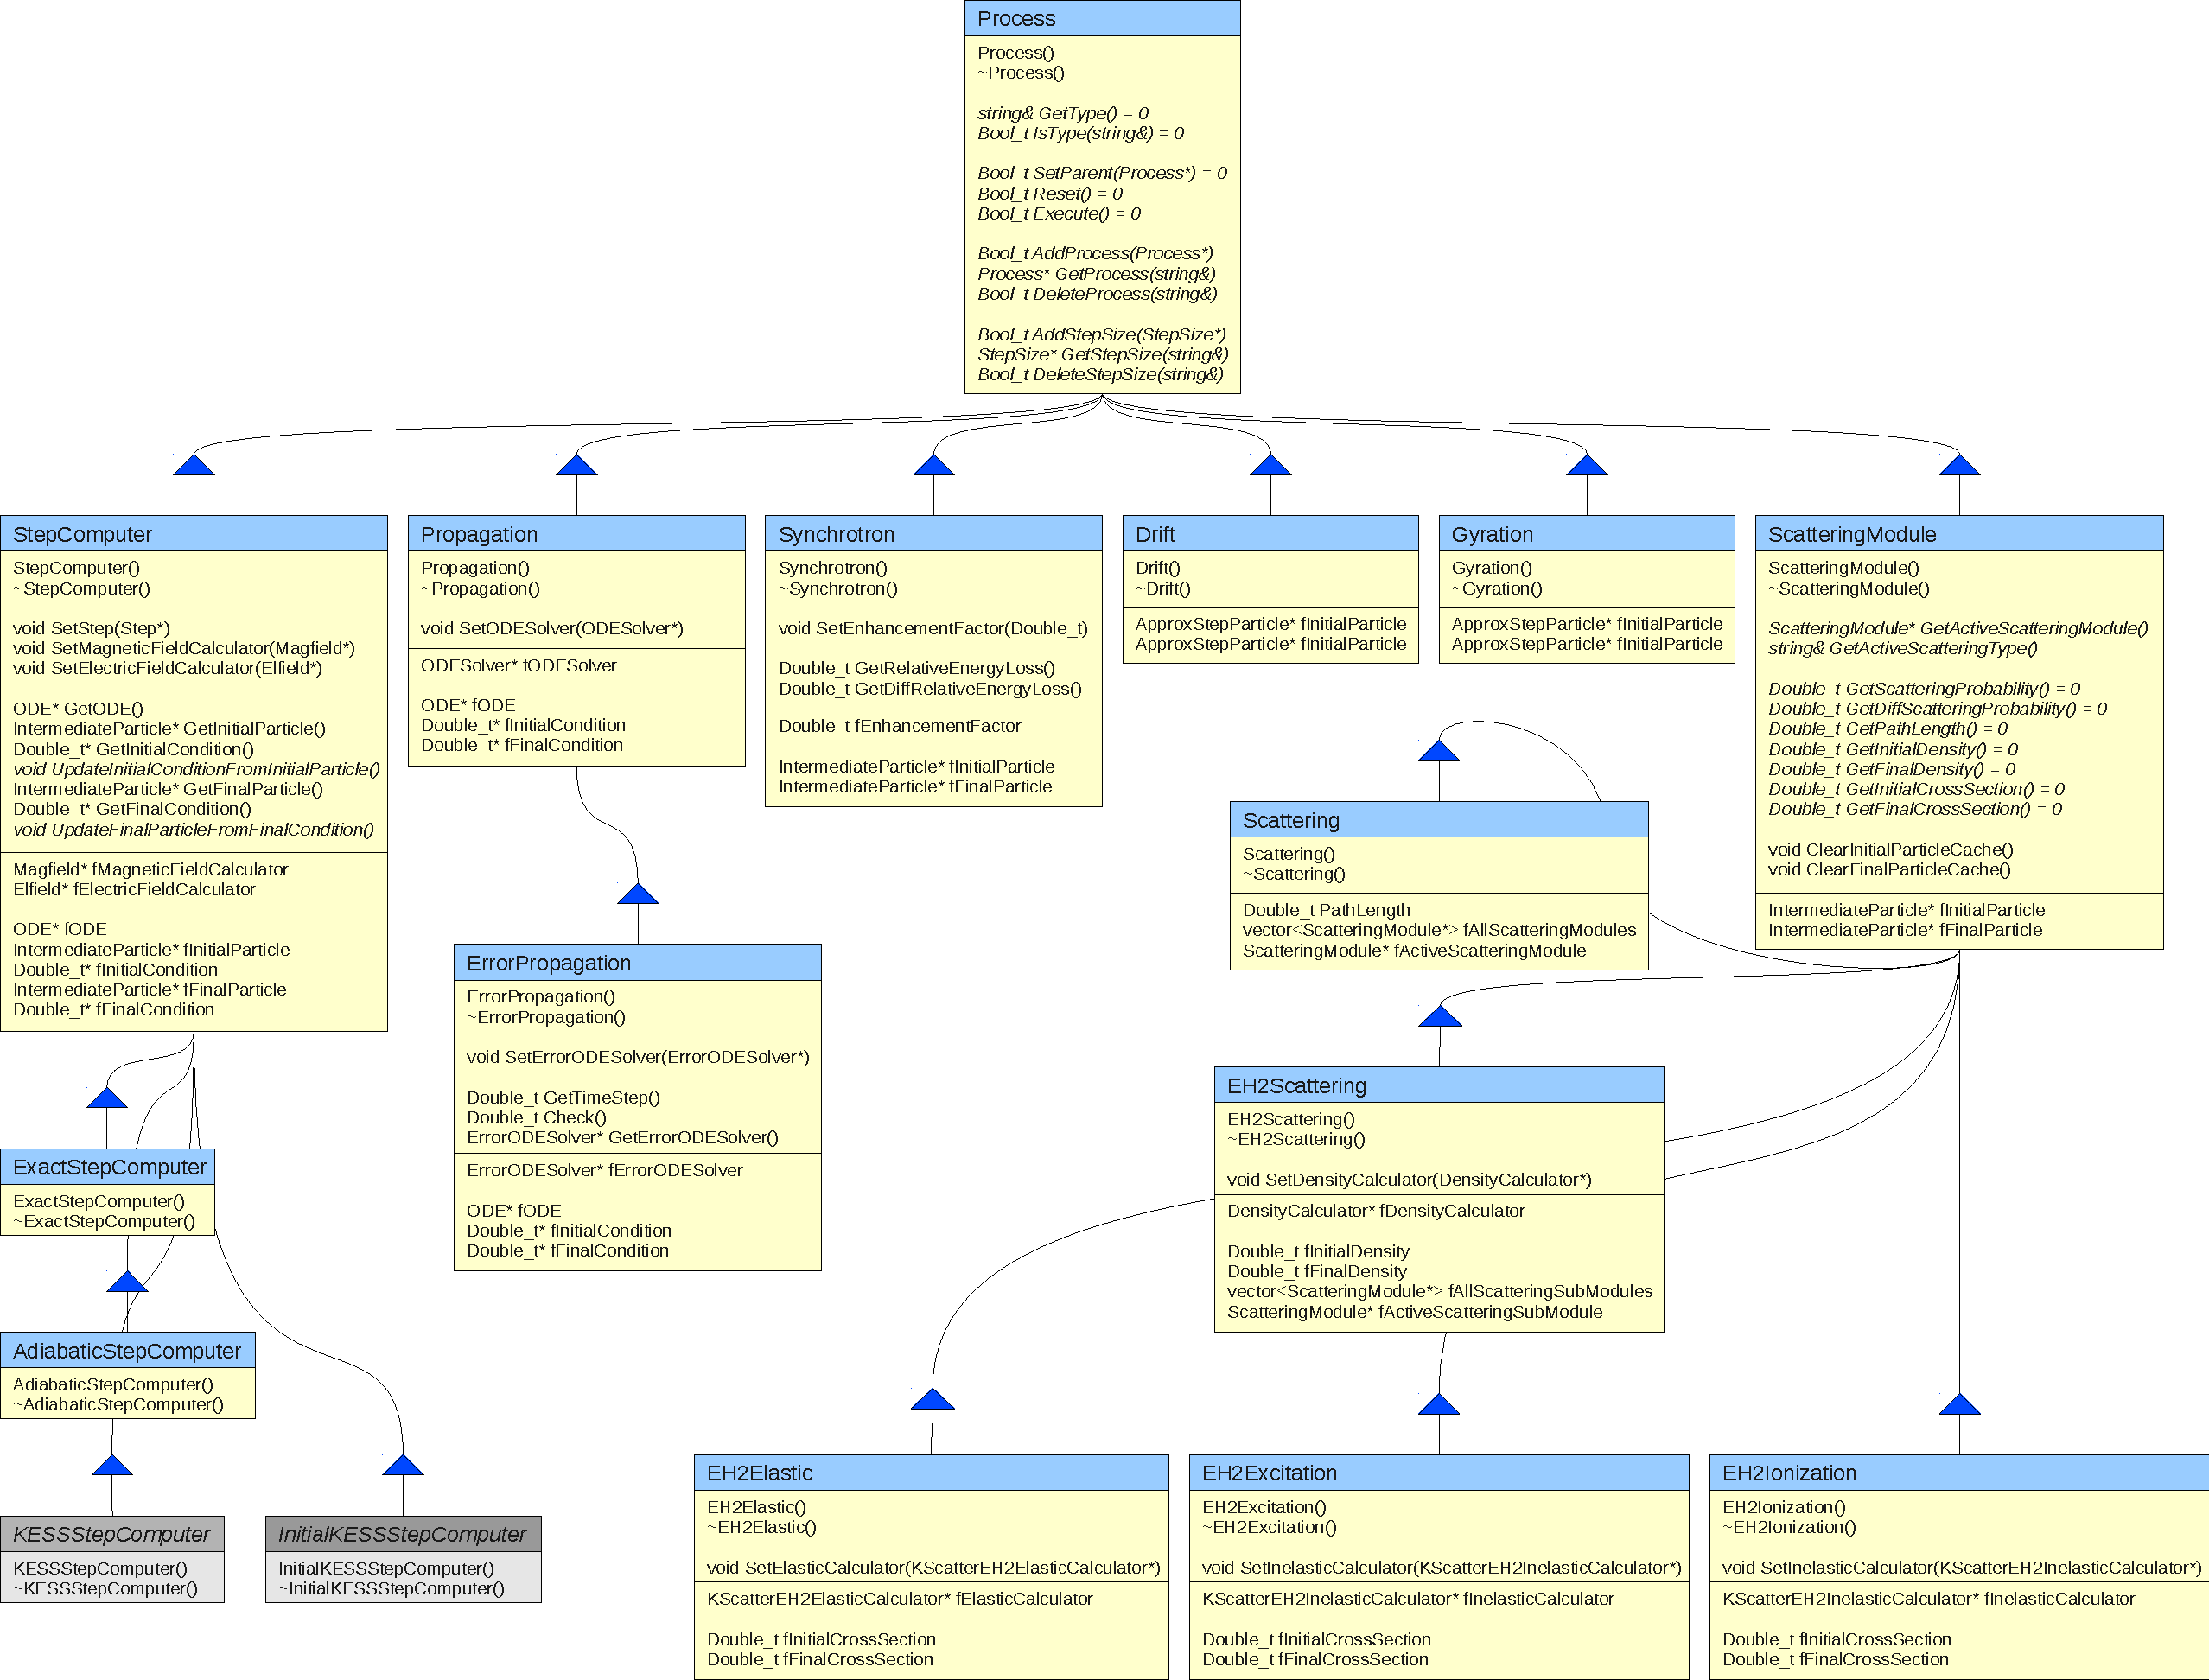
\includegraphics[angle=90,scale=0.58]{./images/KTrackPlots/KTrackProcessInheritance.pdf}
        \caption{Process inheritance diagram for KTrack}
    \end{figure}

\newpage
\thispagestyle{empty}
    \begin{figure}[t]
        \vspace*{-3.5cm}
        \hspace*{-3.2cm}
        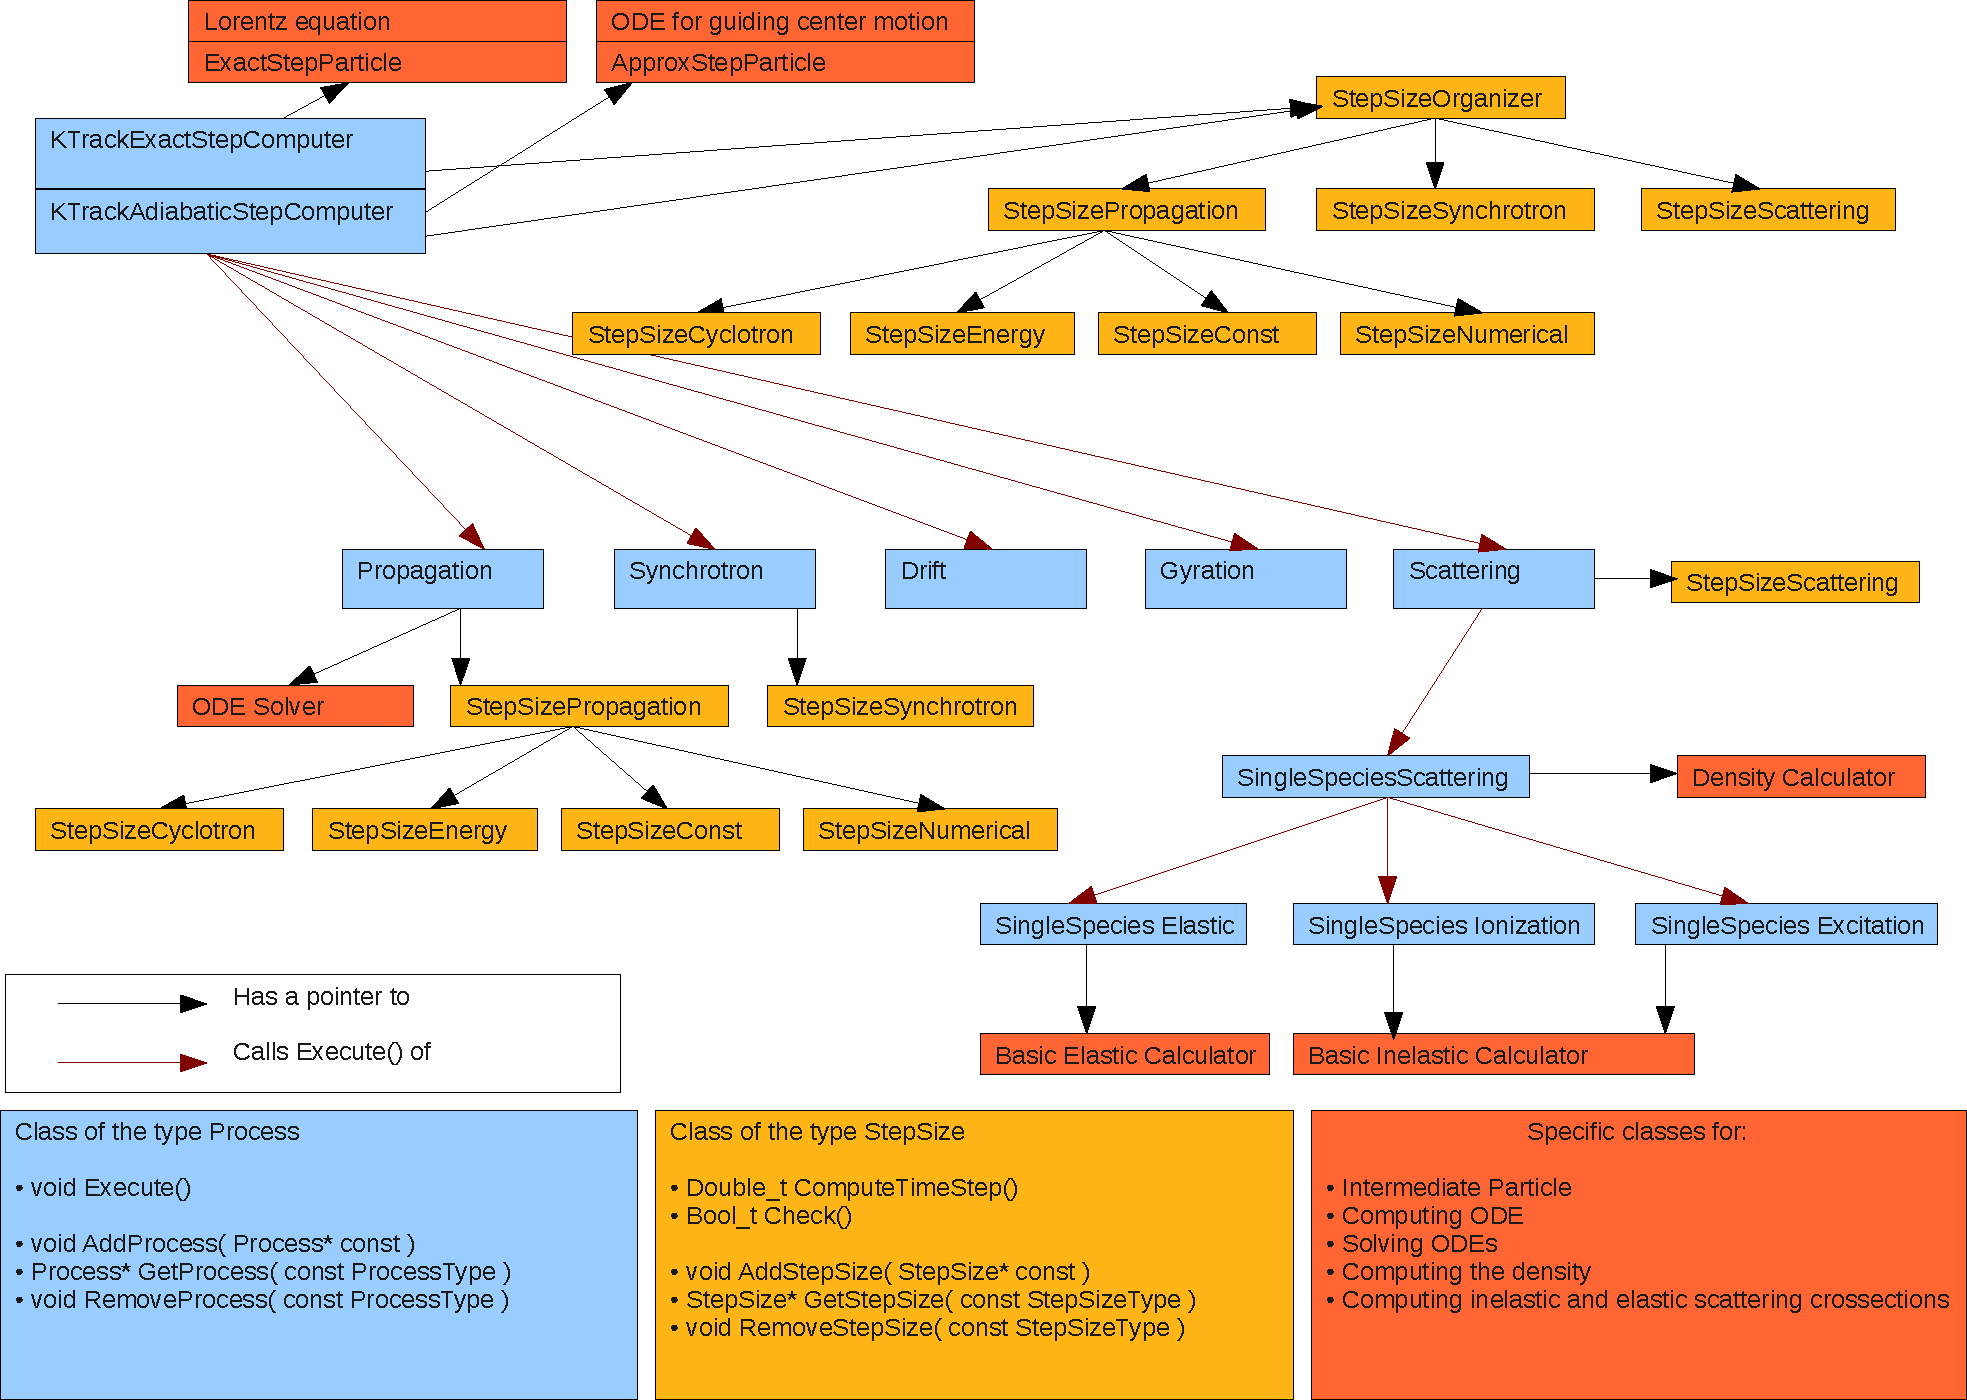
\includegraphics[angle=90,scale=0.75]{./images/KTrackPlots/KTrackDiagramNew.pdf}
        \caption{Collaboration diagram for KTrack}
    \end{figure}


\subsection{Standard test programs}
The purpose of the standard test programs is to give the user and code developer the chance to check whether changes or code developments affected the operability of the program.  

    \subsubsection*{Test against exact track}
    \label{testcompare}
    This test compares different tracking modes against a very accurate exact track. This track is computed using: 
    \begin{itemize}
        \item Exact stepping method
        \item RK8
        \item 48 steps per gyration
    \end{itemize}
    The user can set the conditions for the track that is to be tested:  
    \begin{itemize}
        \item Initial conditions: transmitted or trapped
        \item Stepping method 
        \item ODE solver
        \item Step size control
    \end{itemize}
    When running the test program a trajectory is computed with the chosen method and in addition with the reference settings. At each step of the test trajectory the program determines the position of the particle of the reference track at exactly the time of the test track via interpolation. The absolute value of the difference of the positions is the error.
    
    This test is applicable for short trajectories. For long tracks, e.g. from tracked particles the numerical error of each steps accumulates and will lead to large discripencies between two different tracking methods. Since we do not know the true position of the particle after a long time, another measure of accuracy has to be found. Global variables, like storage time, number of secondary particles, energy loss due to synchrotron, average radius at a given z-position, etc. can be chosen. In section \ref{testtrapped} these tests will be described.
        
    How to use it: Go to directory \textit{Kassiopeia/branches/DanSusanneBranch/bin}. Type \textit{./TestCompareWithExact} this will show you what your options are. Type \textit{./TestCompareWithExact x x x x x x x}, where x is an integer that defines the modes you have chosen. The program writes the deviation of the positions, radius, timestep, etc. between test and reference track into a root file: \textit{Trackxxxxxxx.root}. In addition it automatically creates a plot that shows the deviation over time.
    
    This program was used for testing the operability of the version of KTrack described in this document. In addition the test program was used to test the old version of KTrack. Furthermore, the same analysis was used to cross check old and new KTrack version and singletraj.

    
    \subsubsection*{Test CPT reversal}
    \label{testtime}
     This purpose of this test (\textit{TestCPTReversal}) is to ensure that the KTrack's computational approximations of the underlying
     physical processes do not violate the fundamental symmetries of charge, parity, and time reversal. 
     The user can select the following options to be tested:
    \begin{itemize}
     \item The stepping method: either exact, or using the adiabatic approximation.
     \item The ODE solver
     \item The method of step size control
     \item The electromagnetic field: either uniform constant electric and magnetic fields, or the prespectrometer fields      
    \end{itemize}
    This test program first computes the trajectory of a test particle with the options specified by the user. The
    test particle is an electron, whose initial conditions place it at the origin, with its momentum directed parallel
    to the vector (1,1,1). The electron is propagated for 10$^{5}$ steps and its final position and momentum are recorded.
    Then the test program performs a charge reversal by replacing the electron with a positron, a parity reversal, and a 
    time reversal on the inital conditions and electromagnetic fields. Then the positron is tracked for 10$^{5}$ steps and
    its final position and momentum are compared with that of the previously calculated electron. Since electromagnetism is
    invarient under a simultaneous reversal of charge, parity and time, the final states (position and momentum) of the electron
    and positron should be identical.

    How to use it: From the top level directory go to the \textit{./bin} directory. Type \textit{./TestCPTReversal} to display the available
    options and their corresponding values. Type \textit{./TestCPTReversal x x x x x y} where \textit{x} are the desired option indices
    and \textit{y} is the initial energy of the test particle. The the program will output the final states of the electron and the positron. 
    If their finals states are not identical, or within a very small round off error then some KTrack process has been implemented/changed 
    incorrectly. If further analysis beyond this simple check is desired the trajectory information (x,y,z,t) of the tracked electron
    can be found in a .root file in the same directory with the name \textit{CPTReversalElectronxxxx\_yeV.root}, the track information of 
    the positron is stored in a .root file named \textit{CPTReversalPositronxxxx\_yeV.root}. 
    Note: The synchotron radiation process is not present in this program.      
    
    \subsubsection*{Test of scattering}
    \label{testscatter}
    taken out, since loading pictures caused problems. Will be fixed soon.


    \subsubsection*{Test of synchrotron radiation}
    \label{testtrapped}
    Will be written soon

    
    \subsubsection*{Test of trapped particles}
    \label{testtrapped}
    Will be written soon

\subsection{Tests of KTrack}
    \subsubsection*{Comparison to singletraj}
    
    \textit{Singletraj} is the original tracking program written in C by Ferenc Gl\"uck. A user interface was implemented by Florian Fr\"ankle and Nancy Wandkowsky.
    Four different settings of \textit{singletraj} have been compared to the new KTrack version. 
    \begin{itemize}
        \item Exact stepping mode with fixed time step of $10^{-12} s $.
        \item Exact stepping mode with 32 steps per gyration
        \item Exact stepping mode with energy conservation controlled step size (limits: $10^{-8}, 10^{-12}$)
        \item Adiabatic stepping mode with energy conservation controlled step size (limits: $10^{-8}, 10^{-12}$)
    \end{itemize}
    
    To test the speed of both programs an electron was stored for $10^{-4} s$ in the main spectrometer. The electrons, with the initial conditions :
    \begin{itemize}
        \item $\vec{x}_{\mathrm{start}} = (0,0,0)$,
        \item $E_{\mathrm{kin}_{\mathrm{start}}} = 2000 eV$,
        \item starting angle: $\Phi = 15°$, $\Theta = 0°$
    \end{itemize}
     are magnetically stored between $-9m$ and $+9m$ from the anayzing plane. To get a reliable time measurement the trajectory calculation was repeated ten times and the average run time was computed. Table \ref{speedSingleKTrack} shows the results.
	\begin{center} 
    \begin{table}[t]
        \begin{tabular}{|l||l|l|}
            \hline
             & Singletraj & KTrack \\
            \hline
            \hline
            Exact; Cyclotron & 10.6 s & 5.2 s \\
            \hline
            Exact; Energy & 4.6 s & 2.1 s \\
            \hline
            Adiabatic; Energy & 1.34 s & 0.58 s \\
            \hline
        \end{tabular}
        \caption{This table compares the computation time of singletraj and KTrack. An electron that is trapped for $10^{-4} s$ in the main spectrometer is simulated. See text above.}
        \label{speedSingleKTrack}
    \end{table}
	\end{center}

    
    To test the accuracy, the positions of an electron being transmitted through the main spectrometer are compared. The position is compared at each step and at equal times. The starting conditions of the electrons are:
    \begin{itemize}
        \item $\vec{x}_{\mathrm{start}} = (0,0,-12.5)$,
        \item $E_{\mathrm{kin}_{\mathrm{start}}} = 20000 eV$,
        \item starting angle: $\Phi = 3°$, $\Theta = 0°$ 
    \end{itemize} 

    pictures taken out, since loading caused problems. Will be fixed soon.

\subsection{Technical details}
This chapter will be written in the near future.
    \subsubsection*{Inheritance}
    \label{inheritance}
    \subsubsection*{Const}
    \label{const}
    \subsubsection*{Caching pattern}
    \label{cachingpattern}
    \subsubsection*{Composite pattern}
    \label{compositepattern}    
% KESS documentation for the Kassiopeia Guide



\hypertarget{KESSMain}{}\section{KESS -\/ KATRIN Electron Scattering in Silicon}\label{KESSMain}
\begin{DoxyVersion}{Version}
1.4 \hyperlink{_k_e_s_s_changelog}{ChangeLog} 
\end{DoxyVersion}
\begin{DoxyAuthor}{Author}
Pascal Renschler (\href{mailto:pascal.renschler@ik.fzk.de}{\tt pascal.renschler@ik.fzk.de}) 
\end{DoxyAuthor}
\begin{DoxyDate}{Date}
2008-\/2010 
\end{DoxyDate}
\begin{DoxyAttention}{Attention}
The source of this documentation can be found in: /Modules/Transport/include/KESSRunManager.h. Some links in the Userguide will not work, since there targets are only contained in the Referenceguide.
\end{DoxyAttention}


 KESS (KATRIN Electron Scattering in Silicon) is a true event-\/by-\/event simulation of electrons travelling in and interacting with silicon. The basic geometry setup is a two layer silicon bulk material. The first layer is called Deadlayer and the Second Layer is called Detector or Sensitive Volume. KESS only supports electrons and silicon. It is especially made for low energy electrons with kinetic energies of 0-\/50keV. 

\hypertarget{_k_e_s_s_main_KESSContent}{}\subsection{Content}\label{_k_e_s_s_main_KESSContent}

\begin{DoxyEnumerate}
\item \hyperlink{_k_e_s_s_physics}{Physics} 
\item \hyperlink{_k_e_s_s_simulation}{Simulation} 
\item \hyperlink{_k_e_s_s_changelog}{Changelog} 
\item \hyperlink{_k_e_s_s_history}{History} 
\end{DoxyEnumerate}\hypertarget{KESSPhysics}{}\subsection{Physics}\label{KESSPhysics}
The simulation uses the 2 relevant scattering processes through which low energy electrons interact with solid state silicon. Electrons can scatter elastically or inelastically with silicon, other processes like bremsstrahlung canbe neglected. The transferred energy can then induce follow-\/up processes which are also part of KESS. If the energy transfer is bigger than 0 the Silicon atoms will be exited or ionized. Ionized atoms will mainly relax through Auger or Coster-\/Kronig electron emission and is assumed to be 100\% in the simulation. Relaxation through fluorescence is neglected. The processes included so far are: elastic scattering, inelastic scattering, ionization, atomic relaxation and the vacuum-\/silicon transition probabilities.\hypertarget{_k_e_s_s_physics_elastic}{}\paragraph{Elastic Scattering}\label{_k_e_s_s_physics_elastic}
Electrons scattering with the silicon atom potential will change their direction depending on their energy. The energy lost is negligible. The angular change follows a probability density function derived from calculation or experiment. The data tables used in KESS are calculated with the ELSEPA software \mbox{[}1\mbox{]} using relativistic partial wave expansion model and the Dirac-\/Fock atomic potential. Values are included for 1eV to 400keV.

\mbox{[}1\mbox{]} F. Salvat et al. Comp. Phys. Com. 165 (2005) 157190\hypertarget{_k_e_s_s_physics_inelastic}{}\paragraph{Inelastic Scattering}\label{_k_e_s_s_physics_inelastic}
An incoming electron scattering on other electrons bound in the Silicon (K,L1,L2,L3,M-\/shell) will loose up to half its energy and transfer it to a shell electron. The energy loss is highly dependent on the incoming electron energy. The scattering angle is determined by the found energy loss. Energy transfer to the K and L shell electrons will lead to ionization. A secondary electron is created and is optionally added to tracking (see below). KESS is using tables of the mean free path (MFP) and probability density functions (PDF) based on Penn's formalism \mbox{[}1\mbox{]}. The doubly differntial cross section is given by \[\frac{d^2 \lambda_{in}^{-1}}{d(\hbar \omega)dq} = \frac{1}{\pi a_0 E} Im \{ \frac{-1} {\epsilon(q,\omega)}\} \frac{1}{q}\] where $ \lambda_{in}$ is the electrom MFP, $ \hbar \omega$ is the energy loss, $ q$ is the momentum transfer for an electron with kinetic energy $ E $, $ \epsilon(q,\omega)$ is the dielectroc function, $ a_0$ is the Bohr radius and $ Im \{ \frac{-1} {\epsilon(q,\omega)}\} $ is the energy loss function. The energy loss function can be derived by optical dielectric data $ \epsilon(\omega) $ in the plasmon pole approximation. The optical energy loss function $ Im \{ \frac{-1} {\epsilon(\omega)}\} $can be extended to the electron loss function $ Im \{ \frac{-1} {\epsilon(q,\omega)}\} $ by \[ Im \{ \frac{-1} {\epsilon(q,\omega)}\} = \frac{\omega_0}{\omega} Im \{ \frac{-1} {\epsilon(\omega_0)}\} \] with $ \omega_0$ beeing the positive solution of the dispersion relation \[\omega_q^2(q,\omega_p)=\omega_p^2+\frac{1}{3} \nu_f^2(\omega_p)q^2+(\frac{\hbar q^1}{2m})^2 \] The data to calculate the optical energy loss function was compiled by H. Bichsel \mbox{[}2\mbox{]} from experimental and theoretical sources. The Penn model cross sections describes the effects of bulk plasmon excitations, interband transitions and inner-\/shell ionization. The first and second moment of the doubly differential cross section, is the MFP and the stopping power (SP) accordingly.

The incident electron changes direction after the scattering. The scattering angle relative to the former trajectory of the electron is given by the binary collision model to be \[ sin \theta = \sqrt{\frac{\Delta E}{E} } \] whereas the azimuthal angle can be sampled isotropically from $ \phi = 2\pi R$ with a random number $R $.

\mbox{[}1\mbox{]} D. R. Penn, Phys. Rev. B. 35, 482(1987) \mbox{[}2\mbox{]} H. Bichsel Rev. Mod. Phys. 60 (1988) 3\hypertarget{_k_e_s_s_physics_ionization}{}\paragraph{Ionization of Si atoms}\label{_k_e_s_s_physics_ionization}
Incident electrons can ionize or excite the target atom, depending on the energy transfer $\Delta E $. If an energy transfer from the incident electron to a shell electron $\Delta E>E_{L3}$ the atom is ionized. For smaller $\Delta E $, the the M-\/shell (or valance band) is excited. The electron that was knocked out during the ionization can be treated as a secondary electron (delta ray) and can produce further scattering, ionizations, etc. The secondary electron has the energy $ E=\Delta E-E_b$ where $E_b$ is the according binding energy of the shell electron. The user can choose the polar emission angle $ \theta_e $ and the azimuthal angle $ \phi_e $ of the SE to be determined by two different models. One is called \char`\"{}momentum conservation\char`\"{} and is correlated with the incident electron trajectory and the energy transfer by $ sin \theta_e = cos \theta $ where $ \theta $ is the angle of the incident angle after scattering in relation to its relative direction before the scattering. Since it is a binary collision, the scattering can be described on one plane, therefore the azimuthal angle is $ \phi_e =\pi + \phi $, with $\phi $ beeing the scattering angle of the incident electron.

\mbox{[}1\mbox{]} D. T. Cromer, D. Liberman, LASL report LA-\/4403 (1970)

The second model included as an option is spherical symmetry. Since the emission is happening in a solid, the emission angle can be influenced by other electrons, the nucleus or the crystal lattice. Therefore one can assume that the SE emission is not correlated to the incident electron trajectory at all and therefore violating momentum conservation (at least in a classical two-\/body sense). The according angles would then be calculated with two different random numbers $ R_1 $ and $ R_2 $ to be \[ cos \theta_e=1-2R_1, \phi_e =2\pi R_2.\]\hypertarget{_k_e_s_s_physics_relaxation}{}\paragraph{Atomic relaxation of Si}\label{_k_e_s_s_physics_relaxation}
Ionized Si atoms relax through the Auger and the Coster-\/Kronig effect. The ionized shell is filled by outer shell electrons and the surplus energy is transferred to another electron, which is then emitted. This process continues until all inner shells are filled and is thereby creating a cascade of SE. Auger electrons are emitted in spherical symmetry with an energy $ E_{Auger}=E_X-E_Y $ where $ X $ and $ Y $ are $K $, $L_1 $ or $ L_{2.3}$.

\mbox{[}1\mbox{]} G. W. Fraser et al. Nucl. Instr. Meth. A 350, 368(1994)\hypertarget{_k_e_s_s_physics_KESSTransProb}{}\paragraph{Transmission probability}\label{_k_e_s_s_physics_KESSTransProb}
The base potential for the electron changes when entering or exciting the silicon detector. In KESS this is approximated by a potential step with the height $ \chi $ which is known as the electron affinity. It is defined as $ \chi = E_{Vac} - E_{CBM} $, the difference between the vacuum and the conduction band minimum potential. Especially for true secondary electrons ($E<50$eV) exiting the bulk silicon this effect is very important. The literature value is $ \chi = 4.05$ eV. One must note, that surface contamination (oxides etc.) and electric fields inside the silicon strongly change the shape and the height of the conduction band minimum. This can lead to negative electron affinity (NEA), a slope in $ E_{CBM} $ inside SI and to big gradients close to the silicon surface. The true SE backscattering probability is therefore not a good way to validate this kind of simulations. However, the potential step approximation is included for completeness.

\mbox{[}1\mbox{]} J. M. Fernandez-\/Varea et al., Surf. Interf. Anal. 37, 824(2005) \hypertarget{KESSSimulation}{}\subsection{Simulation}\label{KESSSimulation}
KESS uses a true event-\/by-\/event Monte Carlo model. The electrons are tracked step-\/by-\/step through the silicon. Each step ends with an interaction (elastic or inelastic scattering). After each step various exit conditions are checked. Since many random numbers are used and low energy electron tracks in silicon are very erratic, many electrons with the same starting conditions have to be simulated to reach conclusive results. It is advisable to use parallel computing (e.g. Ruby script etc). The \hyperlink{class_kassiopeia_1_1_k_e_s_s_step}{KESSStep} is the smallest simulation unit. It moves a \hyperlink{class_kassiopeia_1_1_k_e_s_s_electron}{KESSElectron}, determines all relevant processes and saves the information (optional). \hyperlink{class_kassiopeia_1_1_k_e_s_s_track}{KESSTrack} is a collection of \hyperlink{class_kassiopeia_1_1_k_e_s_s_step}{KESSStep} objects and saves information of the beginning and end of the track as well as energy deposition and exit condition. The \hyperlink{class_kassiopeia_1_1_k_e_s_s_track}{KESSTrack} is what most user would like to hae for analysis. Each primary submitted to the \hyperlink{class_kassiopeia_1_1_k_e_s_s_run_manager}{KESSRunManager} creates a primary track. Secondary \hyperlink{class_kassiopeia_1_1_k_e_s_s_electron}{KESSElectron} created by primary collisions and subsequent relaxation are also creating KESSTracks. Since everything interesting is happening during a \hyperlink{class_kassiopeia_1_1_k_e_s_s_step}{KESSStep} here is a little description.\hypertarget{_k_e_s_s_simulation_KESSStep}{}\paragraph{A KESSStep}\label{_k_e_s_s_simulation_KESSStep}
The scattering inside the silicon can be described by the Poisson distribution. The probability $ P $ for a scattering after travelling a distance $ S $between is given by \[ P(S) = \lambda_T^{-1}e^{\frac{-S}{\lambda_t}}\]\hypertarget{_k_e_s_s_simulation_structure}{}\paragraph{Code structure}\label{_k_e_s_s_simulation_structure}
KESS is configured by a Configfile. Please see KESSConfig.txt as an example. The \hyperlink{class_kassiopeia_1_1_k_e_s_s_run_manager}{KESSRunManager} steers the whole simulation and is the interface to the user or other simulations. E.g. you can define KESSElectrons and give them to the RunManager. You can also extract information through the RunManager after each run to use in your own code. An example on how to interact with the RunManager is found in ex1.cxx.

The internal structure is divided into the logical parts: Run (\hyperlink{class_kassiopeia_1_1_k_e_s_s_run_manager}{KESSRunManager}), track (\hyperlink{class_kassiopeia_1_1_k_e_s_s_track}{KESSTrack}) and step (\hyperlink{class_kassiopeia_1_1_k_e_s_s_step}{KESSStep}).

\mbox{[}7\mbox{]} Goto et al. -\/ J. Appl. Phys., Vol. 96, No. 8, 2004 \mbox{[}8\mbox{]} D.C. Joy et al. -\/ Scanning, Vol. 17, No. 5, 2006 \hypertarget{KESSChangelog}{}\subsection{ChangeLog}\label{KESSChangelog}
\hypertarget{_k_e_s_s_changelog_v14}{}\paragraph{KESS 1.4 in Kassiopeia 1.00.00 (under development)}\label{_k_e_s_s_changelog_v14}

\begin{DoxyItemize}
\item passed major physics evaluation (DCJoy, Goto, FPD data, ...)
\item updated documentation and linked to \hyperlink{namespace_kassiopeia}{Kassiopeia}
\item QM transmission and angular change now added for entering silicon as well -\/ needs structural improvement though -\/ the first and last step in Si should be somewhat special and should be reflected in the stepinformation
\item \char`\"{}major\char`\"{} (eV effect) bugfixes regarding band structure and energy point of reference
\item Added bandstructure related parameters to KESSConfig.txt
\item Moved stuff from \hyperlink{class_kassiopeia_1_1_k_e_s_s_run_manager}{KESSRunManager} to \hyperlink{class_kassiopeia_1_1_k_e_s_s_queues}{KESSQueues}, \hyperlink{class_kassiopeia_1_1_k_e_s_s_processes}{KESSProcesses}, \hyperlink{class_kassiopeia_1_1_k_e_s_s_parameters}{KESSParameters} and \hyperlink{class_kassiopeia_1_1_k_e_s_s_run_info}{KESSRunInfo}
\item Spherical symmetry and momentum conservation are now options for knock-\/on secondary production
\end{DoxyItemize}\hypertarget{_k_e_s_s_changelog_v13}{}\paragraph{Version 1.3 (never released)}\label{_k_e_s_s_changelog_v13}

\begin{DoxyItemize}
\item changed \char`\"{}Dapor symmetry\char`\"{} to real spherical symmetry
\item added \hyperlink{class_kassiopeia_1_1_k_e_s_s_navigator}{KESSNavigator} and moved the position calculation etc. to that
\item \hyperlink{class_kassiopeia_1_1_k_e_s_s_electron}{KESSElectron} is now friends with \hyperlink{class_kassiopeia_1_1_k_e_s_s_navigator}{KESSNavigator} (blame D. Furse! Not me!)
\item added Transmission probabilities to \hyperlink{class_kassiopeia_1_1_k_e_s_s_navigator}{KESSNavigator}
\item added PENN CCS
\item extended ELSEPA down to 3eV
\item added abstract class \hyperlink{_k_e_s_s_i_c_s_8h}{KESSICS.h} to handle Ionization probabilities.
\item added KESSPhotoAbsorption process to \hyperlink{_k_e_s_s_i_c_s_8h}{KESSICS.h}
\item removed KESSCrosssections. All CS are registered at \hyperlink{class_kassiopeia_1_1_k_e_s_s_step}{KESSStep} now.
\item backscattering performance tested. PENN, ELSEPA, Relaxation and PhotoAbsorption work fine!
\item added bandGap energy for Si to KESSConfig.txt. Use 0.0 until there is an energy deposition model.
\item added option to just save backscattered electrons in the trackTree to KESSConfig.txt to save harddisk space.
\item KESS is now KATRIN coding standard compliant (sort of)
\end{DoxyItemize}\hypertarget{_k_e_s_s_changelog_v12}{}\paragraph{Version 1.2 (2009-\/10-\/21)}\label{_k_e_s_s_changelog_v12}

\begin{DoxyItemize}
\item cleaned rRunTree
\item made KESSCrossSections.h the wrapper class for all cross sections
\item \hyperlink{_k_e_s_s_e_c_s_8h}{KESSECS.h} and \hyperlink{_k_e_s_s_c_c_s_8h}{KESSCCS.h} are abstract classes for the according cross sections
\item \hyperlink{_k_e_s_s_e_c_s_elsepa_8h}{KESSECSElsepa.h} and \hyperlink{_k_e_s_s_c_c_s_bethe_fano_8h}{KESSCCSBetheFano.h} are the concrete implementations
\item Added option to choose Processes/cross sections to the KESSConfig.txt
\item cleaned StepTree
\item \hyperlink{_k_e_s_s_electron_queue_8h}{KESSElectronQueue.h} can be cleared now
\end{DoxyItemize}\hypertarget{_k_e_s_s_changelog_v11}{}\paragraph{Version 1.1 (2009-\/09-\/02)}\label{_k_e_s_s_changelog_v11}

\begin{DoxyItemize}
\item Changed table lookup routines to STL standard -\/$>$ one run now takes 7\% of the time it used to!!
\end{DoxyItemize}\hypertarget{_k_e_s_s_changelog_v10}{}\paragraph{Version 1.0 (2009-\/08-\/27)}\label{_k_e_s_s_changelog_v10}

\begin{DoxyItemize}
\item Added \hyperlink{class_kassiopeia_1_1_k_e_s_s_primary_track_info}{KESSPrimaryTrackInfo} and KESSRunManager::getLastPrimaryTrackInfo() for implementation in KDES
\item Removed {\itshape SIFermiEnergy\/} -\/$>$ only usage was track killing at LowestEnergyForTracking -\/ SiFermE
\item {\itshape fGlobalElectronID\/} and {\itshape fGlobalTrackID\/} only accessible by KESSRunManager::getNextGlobalTrackID() and KESSRunManager::getNextGlobalElectronID() -\/-\/$>$ controlled by \hyperlink{class_kassiopeia_1_1_k_e_s_s_run_manager}{KESSRunManager} now!
\item Cleaned up \hyperlink{class_kassiopeia_1_1_k_e_s_s_run_manager}{KESSRunManager}
\item Added {\itshape time\/} (absolute time) and {\itshape creationTime\/} to \hyperlink{class_kassiopeia_1_1_k_e_s_s_electron}{KESSElectron}
\item Added \hyperlink{class_kassiopeia_1_1_k_e_s_s_track_info}{KESSTrackInfo}
\item Cleaned up \hyperlink{class_kassiopeia_1_1_k_e_s_s_output}{KESSOutput}
\item \hyperlink{class_kassiopeia_1_1_k_e_s_s_track_info}{KESSTrackInfo} and \hyperlink{class_kassiopeia_1_1_k_e_s_s_primary_track_info}{KESSPrimaryTrackInfo} are now objects that are written to \hyperlink{class_kassiopeia_1_1_k_e_s_s_output}{KESSOutput}. They can also be saved in a queue, if this is required at some point.
\item New option in KESSConfig {\itshape CreatePrimaryTrackTree:1\/} 
\item KESSElectron::move also takes care of timing.
\item You can assign an {\itshape externalID\/} to a \hyperlink{class_kassiopeia_1_1_k_e_s_s_electron}{KESSElectron} which isn't touched by the KESS
\item Check for configFile will now ask for input if it failed
\item a precompiled lib is in ./lib
\item {\itshape kess.cxx\/} and {\itshape KESSConfig.txt\/} moved to examples/
\item {\itshape kess.cxx\/} renamed to {\itshape ex1.cxx\/} 
\item examples now work with {\itshape libKESS.so\/} 
\item Installation section added
\end{DoxyItemize}\hypertarget{_k_e_s_s_changelog_v003}{}\paragraph{Version 0.0.3}\label{_k_e_s_s_changelog_v003}

\begin{DoxyItemize}
\item Added \hyperlink{class_kassiopeia_1_1_k_e_s_s_conf_reader}{KESSConfReader}. You can now use a config file instead of the \hyperlink{class_kassiopeia_1_1_k_e_s_s_run_manager}{KESSRunManager} setters.
\item Added Hack for Martin \char`\"{}Quick'n'Dirty\char`\"{} Babutzka to get energy deposit of last track KESSRunManager::getEDepDetectorOfLastTrack.
\item Now with Uniform exit conditions in \hyperlink{class_kassiopeia_1_1_k_e_s_s_electron}{KESSElectron}
\item Validation of \hyperlink{class_kassiopeia_1_1_k_e_s_s_conf_reader}{KESSConfReader} readin (do the parameters exist?)
\item Added KESSRunManager::setVerbose() 0=none 10=all 
\end{DoxyItemize}\hypertarget{KESSHistory}{}\subsection{History}\label{KESSHistory}
\hypertarget{_k_e_s_s_history_history}{}\paragraph{History}\label{_k_e_s_s_history_history}
The code was originally written in Fortran by Zine-\/El-\/Abidine Chaoui (Physics department, Faculty of Science, University of Setif, Algeria, \href{mailto:z_chaoui@yahoo.fr}{\tt z\_\-chaoui@yahoo.fr}) from 2005 -\/ 2007. It included:
\begin{DoxyItemize}
\item Dirac Partial Wave cross sections for elastic cross sections and Bethe-\/Fano/Penn dielectric formalism for the inelastic cross sections
\item The Bethe-\/Fano inelastic cross sections were calculated by Hans Bichsel (CENPA, University of Washington, Seattle, USA, \href{mailto:bichsel@npl.washington.edu}{\tt bichsel@npl.washington.edu})
\end{DoxyItemize}

Pascal Renschler (Institute for Experimental Nuclear Physics, Karlsruhe Institute of Technology, Germany, \href{mailto:pascal.renschler@gmx.de}{\tt pascal.renschler@gmx.de}) translated the code to c++ starting from 2008:
\begin{DoxyItemize}
\item fully object oriented code structure
\item own electron object
\item \hyperlink{namespace_kassiopeia_1_1_r_o_o_t}{ROOT} random generator (TRandom3.h)
\item full \hyperlink{namespace_kassiopeia_1_1_r_o_o_t}{ROOT} output
\item all processes included as options in the \hyperlink{class_kassiopeia_1_1_k_e_s_s_run_manager}{KESSRunManager}
\item the code is easily parallelized through e.g. a small Ruby script
\end{DoxyItemize}

From 2008 to 2010 Z. Chaoui and P. Renschler included the following:
\begin{DoxyItemize}
\item Ionization process (Fermi Virtual Photon/Photo Absorption Ionization relative probabilities)
\item Relaxation Process (Auger-\/ and Coster-\/Kroning-\/electron emission), fluorescence is excluded
\item Surface escape process
\item Knock-\/on secondary electron emission (spherical symmetry or binary collision model)
\item Secondary cascade
\end{DoxyItemize}

In march 2010 Z. Chaoui and P. Renschler did the following:
\begin{DoxyItemize}
\item extended the elastic cross sections down to 0.1eV
\item major physics evaluation
\end{DoxyItemize}

In September 2010 KESS became a module of \hyperlink{namespace_kassiopeia}{Kassiopeia} (the KATRIN Simulation framework). 







\hypertarget{SSCmain}{}\section{SSC -\/ Source Spectrum Calculation}\label{SSCmain}
\begin{DoxyVersion}{Version}
x 
\end{DoxyVersion}
\begin{DoxyAuthor}{Author}
Markus Hoetzel (\href{mailto:markus.hoetzel@kit.edu}{\tt markus.hoetzel@kit.edu}) 
\end{DoxyAuthor}
\begin{DoxyDate}{Date}
2010
\end{DoxyDate}
\begin{DoxyAttention}{Attention}
The source of this documentation can be found in: /Modules/SSC/include/SSCToolBox.h. Some links in the Userguide will not work, since there targets are only contained in the Referenceguide.

\end{DoxyAttention}

\subsection{Introduction}\label{_s_s_cmain_Introduction}
The parameters of the source have to be known precisely because they are a main systematic uncertainty for the whole measurement of the neutrino mass:

A detailed model of the source is required to investigate the influence of various source parameters. The task of the package \char`\"{}Source Spectrum Calculations\char`\"{} SSC was to combine existing models to one central source model and to implement further models. Former calculations and source models considered the WGTS as a 10 m tube at whole and were not able to account for spatial variations of several source parameters that definitely occur. Dividing the source into small pieces, what is implemented in the developed program code SSC, allows for a very detailed investigation of the influence of source parameters on the integrated beta spectrum. These integrated spectra are calculated for every part of the WGTS using the local physical parameters. A combination of the spectra from all parts of the source gives the spectrum of the whole source, that can be investigated. It is now possible to study the effects of many different source parameters on the integrated beta spectrum of KATRIN. It should be emphasized here that calculations based on distribution functions of the source parameters were performed instead of single particle simulations. The task of SSC in the frame of Kassiopeia is to provide a realistic source model for the particle generators of KPAGE to simulate electrons from the source through the spectrometers to the detector using one program: Kassiopeia.
\subsection{General: WGTS}\label{_s_s_cmain_summaryWGTS}
The Windowless Gaseous Tritium Source WGTS contains the molecular tritium to investigate its beta spectrum near the endpoint. The WGTS is a 16 m long cryostat with a central region of 10 m, containing the beam tube with a diameter D=90 mm and a differential pumping subsection at the front side, the DPS1-F and at the rear side, the DPS1-R. In the middle tritium is injected via 500 holes into the beam tube, flows towards both ends of the WGTS and can decay during this time. The created electrons are guided by magnetic field lines provided by superconducting solenoids out of the source towards the spectrometer where the energy is analysed. The tritium that does not decay reaches the pump ports and is pumped out. To further reduce the tritium flow towards the spectrometer a differential and a cryo pumping subsection are used.

An important quantity describing the WGTS is the column density $\rho d$, the integrated density of the source along the beam axis z. For the WGTS $\rho d = 5\cdot 10^{17} \rm{cm}^{-2} $ will be used. This ensures reasonable high activity together with a sufficient amount of electrons ($ P_0 = 41.7\,\%$) that leave the source without energy loss due to inelastic scattering at the remaining tritium molecules. For the determination of the neutrino mass, it is very important to maintain a stable column density on a 0.1\%-\/level at any time. Otherwise, the systematic effect on mnu2 gets intolerably large. The column density is affected by beam tube geometry, tritium injection pressure $p_{in}$, throughput $q$, temperature profile and other parameters. Numerical calculations provide the column density for the specified source parameters.

\subsection{General: Concepts}\label{_s_s_cmain_generalConcepts}
The following sections contains main concepts of KATRIN especially of the WGTS that are needed throughout SSC. Look at the Kassiopeia ReferenceGuide to find more information (class descriptions) how these concepts are used by SSC.
\subsubsection{Integrated betaspectrum}\label{_s_s_cmain_intbetaspec}
KATRIN will measure the integrated betaspectrum \[ N(qU, E_0, m^2_\nu) = N_{\rm{tot}} t_U \int^{E_0}_0 \frac{dN}{dE}(E_0, m^2_\nu) \cdot R(E, qU) dE \] to determine the neutrino mass square mnu2. The count rate N depends on the retarding potential qU, the endpoint $E_0$ of the differential betaspectrum $dN/dE$, the number of tritium nuclei in the source $N_{tot}$, the measuring time $t_U$ and the response function $R$ of the experiment.\par
 To extract $m_{\nu}^2$ from the measurements, the chisquare-\/function for the parameters $E_0$, $m_{\nu}^2$, signal strength $R_s$ and background contribution $R_b$ is minimized. Marginalisation of the unwanted parameters $E_0$, $R_s$ and $R_b$ yields the most probable value of $m_\nu^2$.\par
 SSC can calculate the integrated spectrum measured by KATRIN for different values of the source parameters and investigate their effects.

\subsubsection{Differential betaspectrum}\label{_s_s_cmain_diffbetaspec}
For the desciption of the differential betaspectrum according to Fermi's theory, SSC uses \[ \frac{dN}{dE}=C\cdot F(Z,E)\cdot p_e \cdot (E + m_e c^2)(E_0-E)\sqrt{(E_0-E)^2-m_{\nu}^2 c^4}\,\Theta(E_0-E-m_\nu c^2). \label{eq:diffbetaspektrum} \] C is a constant \[ C= \frac{G_F^2\cos^2{\theta_C}}{2\pi^3\hbar^7 c^5}(g_V^2 + 3g_A^2) \label{eq:betakonstante} \] with Fermi constant $G_F$, Cabibbo angle $\theta_C$ and the coupling constants $g_V$ and $g_A$ for the weak interaction. F(Z,E) is the Fermi function, $E_0$ is the endpoint, $m_{\nu}^2$ is the neutrino mass square. $p_e$ as momentum and $E$ as kinetic energy of the electron are kinematic quantities. The Fermi function is used as in \mbox{[}1\mbox{]} \[ F(Z,E)=\frac{x}{1 - e^{-x}}\cdot(a_0 + a_1 \beta), ~~~~ x = \frac{2\pi Z \alpha}{\beta} \] with $\beta=\frac{v}{c}$ and the empirical values $a_0 = 1,002037$ and $a_1 = -0,001427$.

A more detailed description needs some corrections that will be discussed in the following sections or directly in class documentations of the reference guide. 

\mbox{[}1\mbox{]} K. Eitel et al., \char`\"{}Estimate of the KATRIN sensitivity on the neutrino mass\char`\"{}, KATRIN Report, 65-\/SRP-\/4011-\/1, 2003.

\paragraph{Radiative corrections}\label{_s_s_cmain_radcorr}
The influence of virtual and real photons on the spectrum is considered by multiplication of $dN/dE$ with the radiative corrections \mbox{[}2\mbox{]} 
\begin{equation}
	\begin{split}
	f_{\text{rad}}(E) = (W-\epsilon)^{(2\alpha / \pi) t(\beta)} &\left[ 1 + \frac{2\alpha}{\pi} \left\{ t(\beta)\left[ \ln 2 - \frac{3}{2} + \frac{(W-\epsilon)}{\epsilon}\right] \right. \right. \\ & + \frac{1}{4}[t(\beta) + 1]\left[2 (1 + \beta^2) + 2 \ln(1-\beta) + \frac{(W-\epsilon)^2}{6\epsilon^2}\right] \\ & \left. \left. - 2 + \frac{1}{2} \beta - \frac{17}{36} \beta^2 + \frac{5}{6} \beta^3 \right\}\right] 
	\label{eq:radcorrection}
	\end{split} 
\end{equation}

\[ \rm{with}~~W=\frac{E_0 + m_e c^2}{m_e c^2},~~~ \epsilon = \frac{E + m_e c^2}{m_e c^2},~~~ \beta = \frac{pc}{E + m_e c^2},~~~ t(\beta) = \frac{1}{2\beta} \ln \frac{(1+\beta)}{(1-\beta)}. \]

\mbox{[}2\mbox{]} W.W. Repko, C. Wu, "Radiative corrections to the end point of the tritium betadecay spectrum , Phys. Rev. C28 (1983) 2433.

\paragraph{Tritium purity}\label{_s_s_cmain_epstrit}
The tritium purity of the injected gas defines aside the injection pressure and throughput the number of tritium molecules in the WGTS and has to be known with an accuracy of 0.1\%. Additionally, the Final State Distributions (see next subsection) of the molecules DT and T2 are different.\hypertarget{_s_s_cmain_fsd}{}

\paragraph{Final State Distribution}\label{_s_s_cmain_fsd}
If molecular T2 decays \[ \rm{T}_2\,\rightarrow\,^3\rm{HeT}^+ + \rm{e} + \overline{\nu_{\rm{e}}} \] energy remains at the daughter nucleus 3HeT+ in rotational, vibrational and electronic excitations. This amount of energy is not transferred on the electrons and thus is impossible to detect. But the final states of the daughter molecules can be calculated \mbox{[}3\mbox{]},\mbox{[}4\mbox{]} and used as a Final State Distribution FSD. The differential betaspectrum (including radiative corrections f\_\-rad) is extended to 

\begin{equation}
	\begin{split}
	\frac{dN}{dE} =& \;C\cdot F(Z,E)\cdot p \cdot (E + m_e c^2)\cdot f_{\text{rad}}(E) \cdot \sum_f [ P_f \cdot(E_0 - E_f -E)\, \cdot  \\
	&  \sqrt{(E_0 - E_f -E)^2 - m_\nu^2 c^4} \cdot \Theta(E_0 -E_f -E - m_\nu c^2)\,].
	\end{split}
	\label{eq:spektrumFSD}
\end{equation}

SSC also uses the FSD of the decay of DT and weights the FSD according to the tritium purity to get an effective FSD for the WGTS.

\mbox{[}3\mbox{]} N. Doss et al., \char`\"{}Molecular effects in investigations of tritium molecule \$$\backslash$beta\$ decay endpoint experiments\char`\"{}, Phys. Rev. C 73 (2006) 025502.\\
 \mbox{[}4\mbox{]} N. Doss and J. Tennyson, \char`\"{}Excitations to the electronic continuum of 3HeT+ in investigations of the T2 beta-\/decay experiments\char`\"{}, J. Phys. B: At. Mol. Opt. Phys. 41 (2008) 125701.

\paragraph{Doppler smearing}\label{_s_s_cmain_doppler}
The thermal movement of the tritium molecules and an additional velocity due to the tritium circulation cause a Doppler smearing of the electron energy spectrum. Because the velocities of the molecules in the whole WGTS differ (see section \char`\"{}Velocity profile\char`\"{}), the spectrum of every part of the WGTS has to be smeared separately.


\subsubsection{Magnetic field}\label{_s_s_cmain_magneticfield}
The magnetic field needed in SSC is provided by Kassiopeias FieldCalculators. A real profile is used instead of a constant value $B_S=3.6$\,T, so the electrons of different parts of the WGTS are emitted under different maximal opening angles \[ \theta_{\rm{max}} = \arcsin\left(\frac{B_S}{B_{\rm{max}}}\right) \] which influences the scattering probabilities.

\subsubsection{Temperature profile}\label{_s_s_cmain_temperatureprofile}
The temperature of the beam tube is not homogeneous: The thermal radiation through the pump ports at the end of the 10\,m beam tube will heat the inner surface and create a longitudinal temperature profile. In addition the cooling system aligned on both sides of the beam tube will create a radial and azimuthal temperature profile. A temperature profile also affects the density profile and velocity profile \mbox{[}5\mbox{]}, \mbox{[}6\mbox{]}.

\mbox{[}5\mbox{]} F. Sharipov, \char`\"{}Numerical calculation of tritium flow through the KATRIN beam line.\char`\"{}, KATRIN Report, 2003.\\
\mbox{[}6\mbox{]} F. Sharipov et al., \char`\"{}Influence of temperature variations and acoustic waves on the column density. Calculations of the velocity distribution function.\char`\"{}, KATRIN Report, 2009.

\subsubsection{Velocity profile}\label{_s_s_cmain_velocityprofile}
In a closed system of temperature $T_0$ the velocities of molecules of mass m follow a Maxwellian distribution around the most probable molecular speed $ v_0 = \sqrt{2 k_B T_0 / m}$. The tritium circulation adds a directional bulk velocity $U_z$ to the thermal motion, so the distribution is approximated by a local Maxwellian \mbox{[}6\mbox{]} \[ f(\vec{r}, \vec{v}) \approx \frac{\rho(z)}{(\sqrt{\pi}v_0)^3} \exp \left[-\frac{v_r^2+v_\phi^2+(v_z-U_z)^2}{v_0^2}\right], \label{eq:lokalMB} \] with the local density $\rho(z)$ and the velocity components $v_r$, $v_\phi$ and $v_z$ in cylindrical coordinates. The bulk velocity U\_\-z depends on the position in the source: \[ U_z(z,r,\delta)=-v_0\xi_p(z)\left[a(\delta) - c(\delta)\cdot \left(\frac{r}{R}\right)^2\right] \] with the pressure gradient $\xi_p(z)= \frac{R}{\rho(z)}\frac{d\rho(z)}{dz}$ and the coefficients \[ a(\delta)=\left[0.894 - 0.1048 \delta \left(1-\frac{\ln \delta}{4}\right)\right]\frac{1 + \delta}{1+1.963\delta}+ \frac{\delta(\delta+2.036)}{2.593+4\delta} \] \[ c(\delta)= \left[0.295 - 0.0536 \delta\left(1- \frac{\ln \delta}{4}\right)\right]\frac{1 + \delta}{1+ 0.7599\delta}+ \frac{\delta^2}{0.07788 + 4\delta}. \] that have been calculated in \mbox{[}6\mbox{]}. These coefficients have to be calculated only once as a function of the rarefaction parameter (see below). If the velocity profile is known, the Doppler smearing can be calculated for every position inside the WGTS.


\subsubsection{Density profile}\label{_s_s_cmain_densityprofile}
In the middle of the WGTS, tritium is injected, at the ends turbo molecular pumps pump out the gas. A density profile along the axis between injection and the pump ports will be reached.

The rarefaction parameter is defined as \[ \delta(z) = \frac{R \cdot P(z) }{ \mu_0 \cdot v_0}. \label{eq:rarefaction} \] with inner radius R of the beam tube, pressure $P$ and viscosity $\mu_0$. In the WGTS $\delta$ varies from $\delta_{\rm{in}}=21.67$ at the injection point (hydrodynamical regime) to $\delta \ll 1$ at the first pump port (free-\/molecular flow). The transitional regime in between makes the calculation of the density profile complicated. Additionaly a longitudinal or even radial/azimuthal temperature profile will modify the density profile.\par
 At present, different density profiles can be used, please look at class documentations for further information. With a longitudinal temperature profile, the density profile is modified. A C++ version of a FORTRAN program by F. Sharipov is used to numerically calculates the density profile for a given temperature profile.

\subsubsection{\char`\"{}Slicing\char`\"{}}\label{_s_s_cmain_slicing}
To account for all spatial variations (see above) of the source parameters, SSC can divide the WGTS into many small parts, so called source pixels. First, a longitudinal partition in thin slices divides the 10 m of the beam tube. At present the slices are equidistant, but their widths can easily be adapted to study specific problems. Every slice can then be divided into one center region with 4 pixels and 12 rings of which every ring is divided into 12 pixels. This segmentation is based on the detector design. If the magnetic fields at the source and at the detector are known, it is be possible to calculate which parts of the source are mapped to which detector pixel.

\subsubsection{\char`\"{}Rebinning\char`\"{}}\label{_s_s_cmain_rebinning}
The calculation of the WGTS spectrum consists of the calculation of the spectrum of each source pixel. If only few longitudinal slices are used, e.g. 10, the scattering probabilities are inaccurate. Normally, 1000 slices, where each has 12 rings and each ring consists of 12 pixels, are used, but that needs a lot computing time. To reduce this time, it is possible to combine some neighbored longitudinal slices after calculation of the individual scattering probabilities without losing precision. For example, one can easily reduce 1000 longitudinal slices to 10 rebinned longitudinal slices. This procedure is implemented in SSC.

\subsubsection{Response function}\label{_s_s_cmain_response}
The response function R \[ R(E, qU) = \int_0^{E/2} T(E, qU) \cdot(P_0 \delta(\varepsilon) + P_1 f(\varepsilon)+P_2(f\otimes f)(\varepsilon)+ \cdots)d\varepsilon . \] combines the scattering probabilities P\_\-i, the convolutions of the energy loss function (see below) and the transmission function

\begin{equation}
	T(E, qU) = \begin{cases}
	0				& E-qU \leq 0 \\
	\frac{1-\sqrt{1-\frac{E-qU}{E}\frac{B_S}{B_A}}}{1-\sqrt{1-\frac{\Delta E}{E}\frac{B_S}{B_A}}} & 0<E-qU\leq\Delta E \\
	1					&	E-qU > \Delta E.
	\end{cases}
	\label{eq: Transmissionsfunktion}
\end{equation}

The response function determines the probability that an electron emitted in the source with energy E running against the spectrometer potential $qU$ will reach the detector. For e.g. 10 longitudinal slices, every slice j has its own set of scattering probabilities $(P_i)_j$ and thus its own response function.
\begin{figure}[ptb]%
  	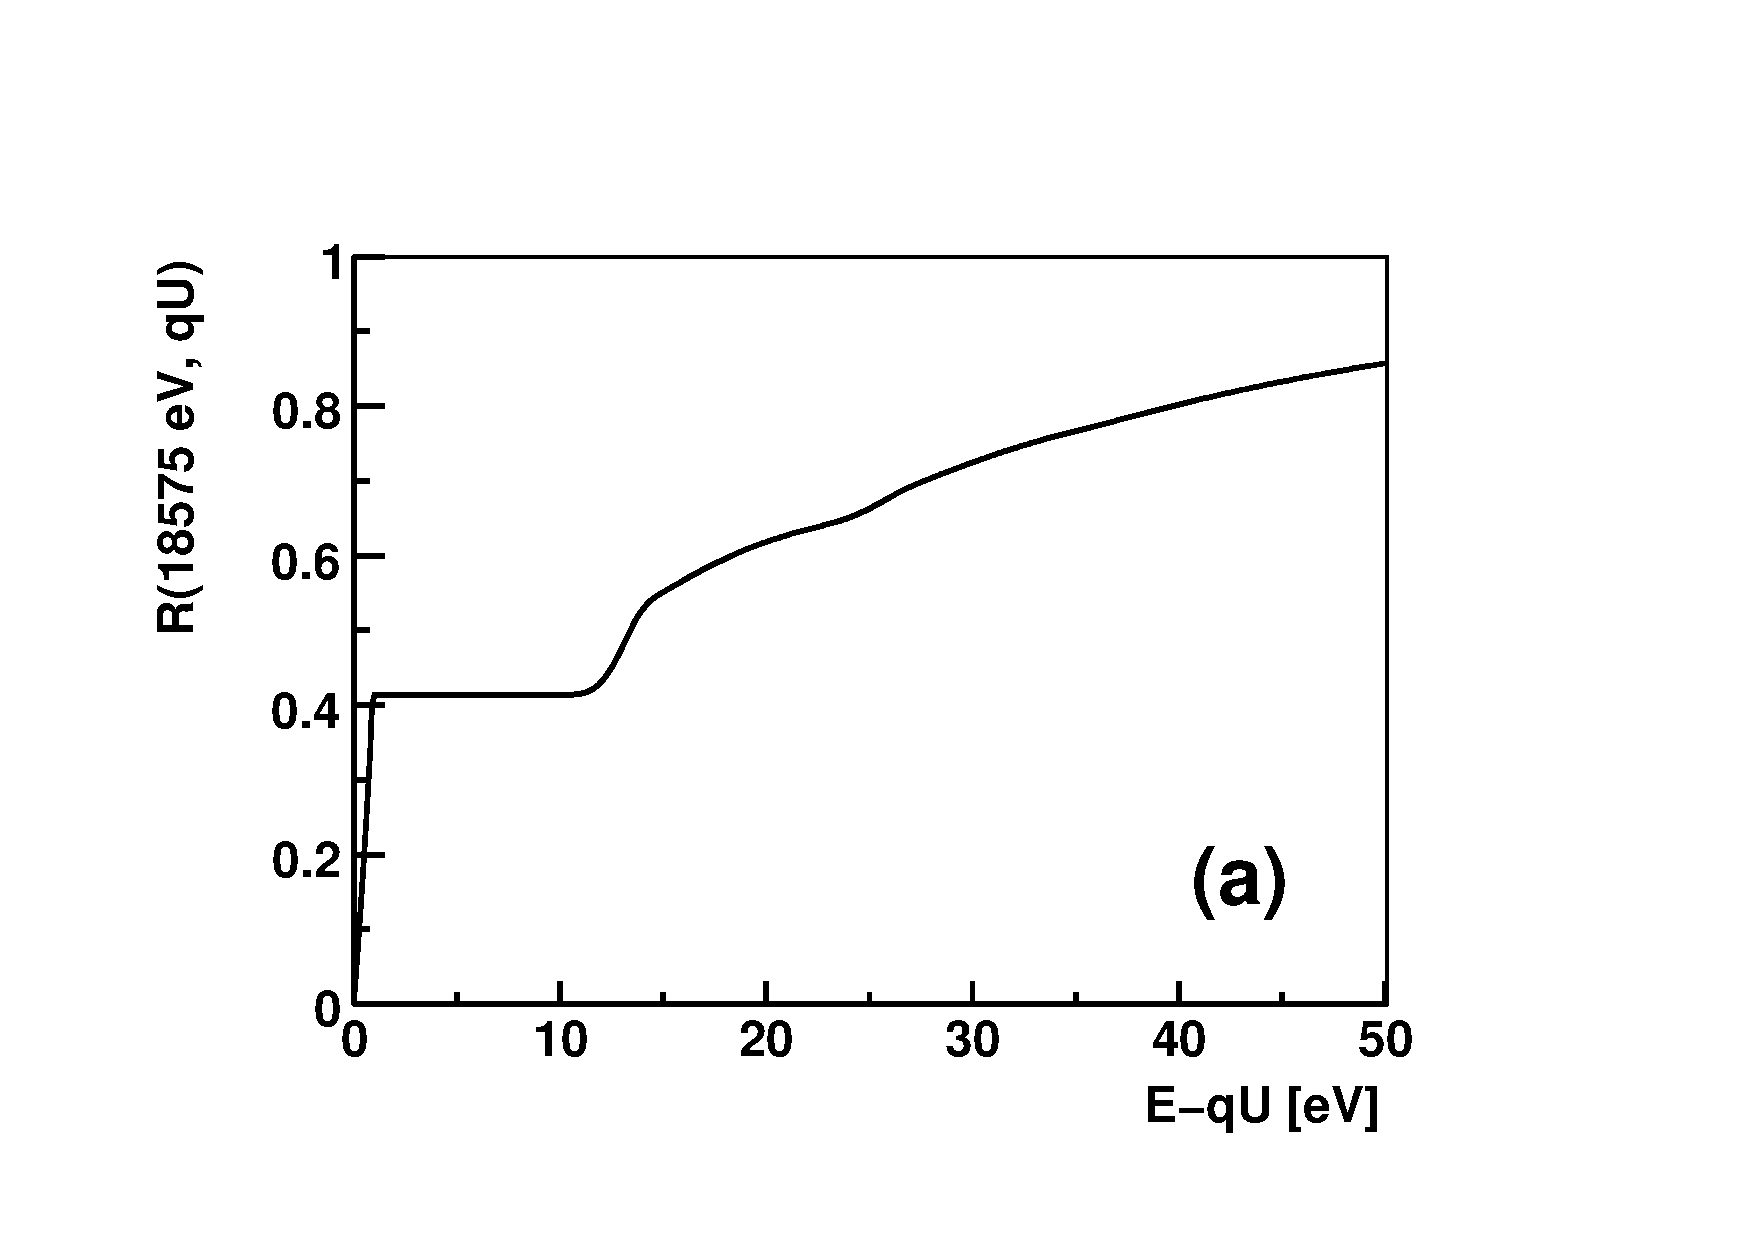
\includegraphics[width=0.50\columnwidth, trim= 40 40 40 40, clip]{images/SSCPlots/responsefunction.pdf}%
	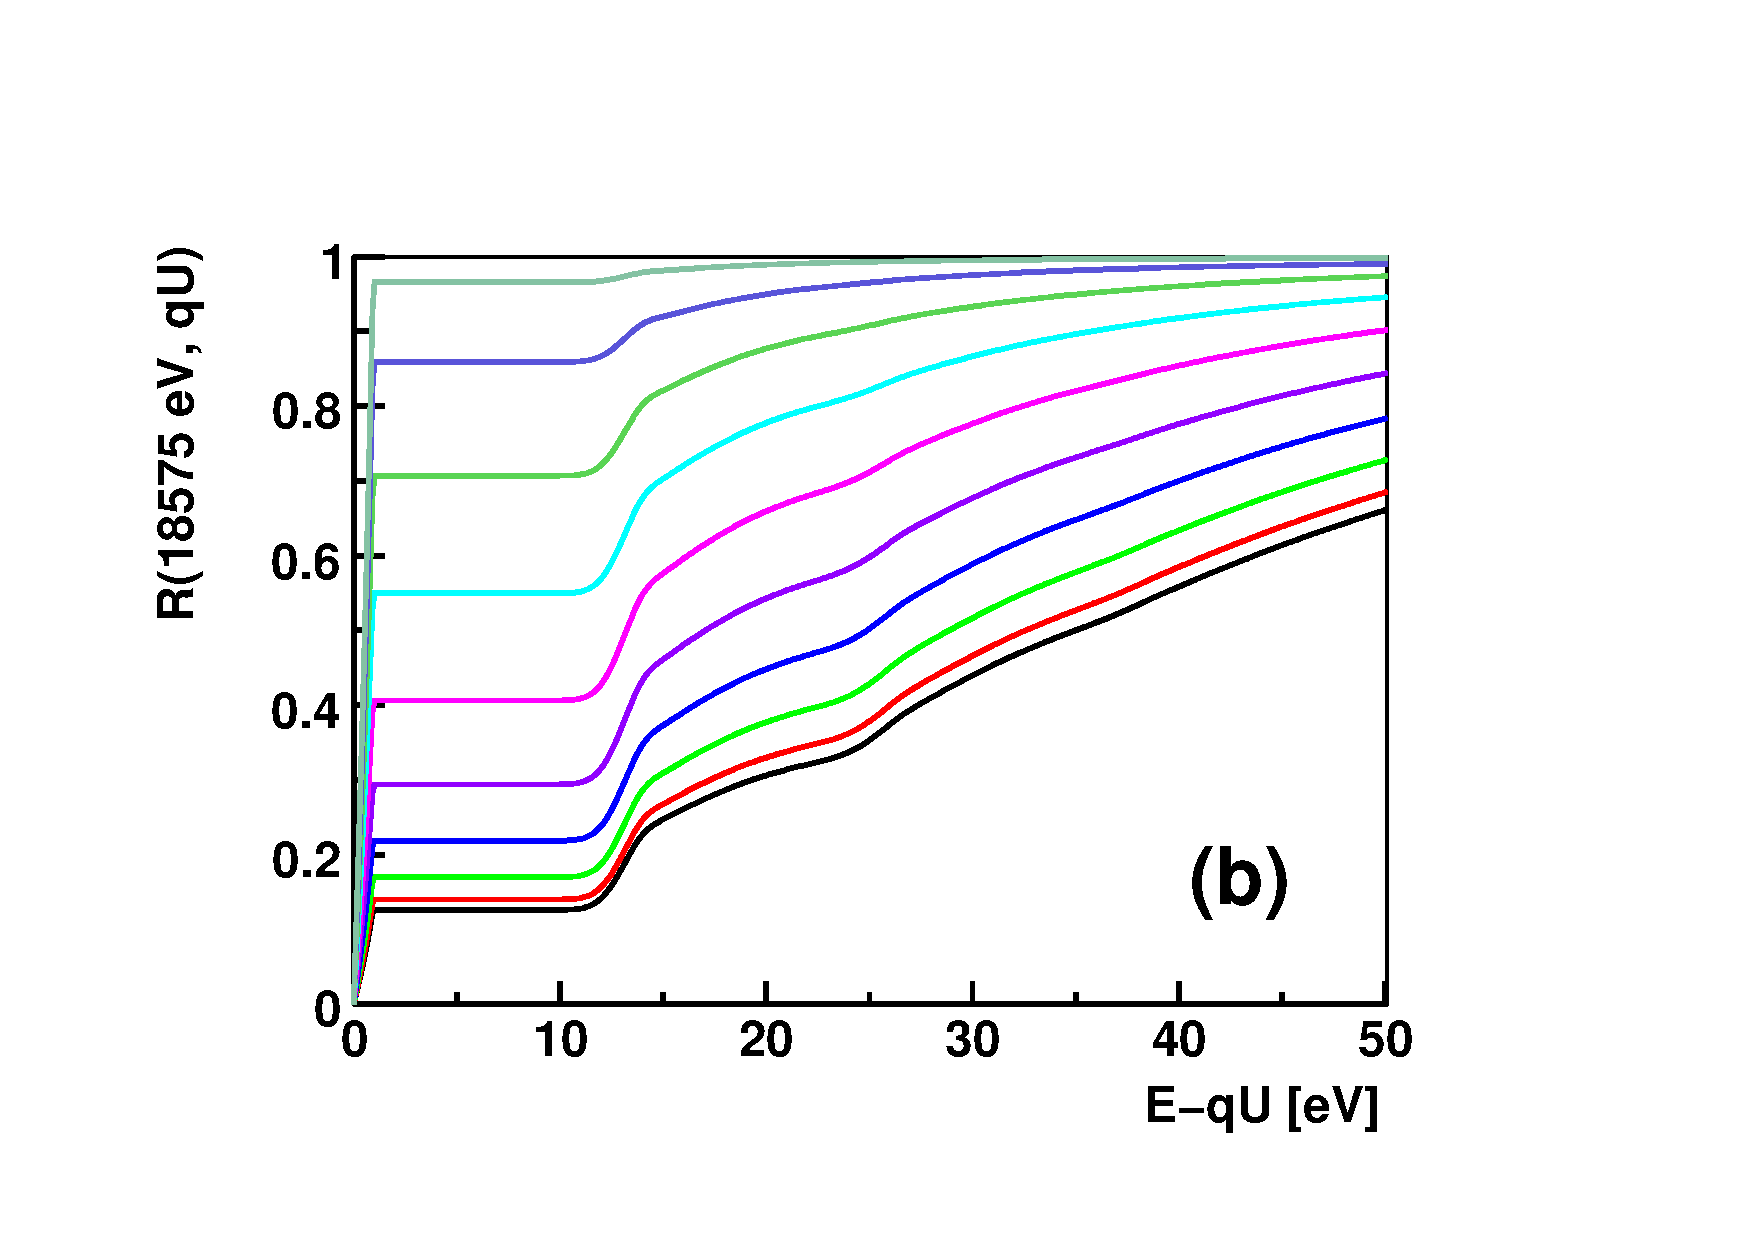
\includegraphics[width=0.50\columnwidth, trim= 40 40 40 40, clip]{images/SSCPlots/responseeverybin.pdf}%
	\caption{\textbf{(a) KATRIN standard response function $R(E,qU)$ and (b) individual response function for 10 rebinned longitudinal source pixel.}}%
	\label{fig:Response10bins}%
\end{figure}


\paragraph{Energy loss and scattering probabilities}\label{_s_s_cmain_eloss}
Inelastic scattering must be considered, since electron scattering inelastically at tritium molecules lose energy according to the energy loss function
\begin{equation}
	f(\epsilon)= \begin{cases}
	A_1 \exp\left(-\frac{2(\epsilon - \epsilon_1)^2}{\omega_1^2}\right)   & \, \epsilon < \epsilon_c \\
	A_2 \frac{\omega_2^2}{\omega_2^2 + 4 (\epsilon - \epsilon_2)^2} & \, \epsilon \geq \epsilon_c
	\end{cases}
	\label{eq:Energieverlust}
\end{equation}

with the parameters $A_1=0,204\pm0,001$, $\omega_1=1,85\pm0,02$, $A_2=0,0556\pm0,0003$, $\omega_2=12,5\pm0,1$, $\epsilon_1=12,6$, $\epsilon_2=14,30\pm0,02$ and $\epsilon_c=14,09$. The minimal energy loss for one scattering is 10 eV.

Furthermore multiple scattering is possible. To get the fraction of electrons that scatter i-\/times, the scattering probabilities P\_\-i are used: \[ P_i=\frac{1}{\rho d(1-\cos \theta_{\rm{max}})} \int_{-5m}^{+5m}dz \int_0^{\theta_{\rm{max}}} d\theta \rho(z)P_i(z,\theta)\sin\theta. \] with the column density $\rho d$, the maximal opening angle $\theta_{\rm{max}}$ and \[ P_i(z, \theta)=\exp (-\lambda \sigma_{\rm{tot}}) \frac{(\lambda \sigma_{\rm{tot}})^i}{i!} \] \[ \lambda(z, \theta) =\frac{1}{\cos \theta} \int_z^l\rho(z')dz' \] $P_i(z, \theta)$ describes the probability of an electron emitted at position z under angle $\theta$ to scatter i-\/times. $P_i(z, \theta)$ follows a Poisson distribution. $\lambda(z, \theta)$ describes the number of molecules passed by an electron during his cyclotron motion ($1/\cos{\theta}$) between emission point and spectrometer.$\backslash$ The values P\_\-i can be calculated for each part of the WGTS separately and can be used to get a specific response function. This description is more detailed than just know average values for the whole WGTS \[ P_0 = 0.413339, ~~ P_1 = 0.292658, ~~ P_2 = 0.167331, ~~ P_3 = 0.079129, ~~ P_4 = 0.031776. \]

Energy loss due to synchrotron radiation has not been considered yet, because the program uses no information on track lengths of the electrons within the magnetic fields. 

% DAQ documentation for the Kassiopeia Guide

\section{Data Acquisition}\label{sec:DAQ}

%% Programming guide for the Kassiopeia Guide
\chapter{Programmer's Guide}\label{ch:programmersguide}

%\section{All You Need to Know to Become a Kassiopeia Programmer}%\label{sec:Programming}
Comming Soon!

\bibliography{KSGuide}

\end{document}  
